%This is a comment, it will not be compiled...

\listfiles
\documentclass[12pt]{report}
\usepackage[intoc]{nomencl}

\textwidth=6in
\oddsidemargin=0.2in
\topmargin=-0.5in
\textheight=9in  % 9in must include page numbers
\textfloatsep=0.4in \addtocontents{toc}{\vspace{0.4in} \hfill
Page\endgraf} \addtocontents{lof}{\vspace{0.2in} \hspace{0.13in} \
Figure\hfill Page\endgraf} \addtocontents{lot}{\vspace{0.2in}
\hspace{0.13in} \ Table\hfill Page\endgraf}

%\usepackage{enumitem}
\usepackage{hyphenat}
\usepackage{siunitx}
\usepackage{fancyvrb}
\usepackage{amsmath}
\usepackage{rotating}
\usepackage[export]{adjustbox}
\usepackage[T1]{fontenc}
\usepackage{textcomp}
\usepackage{array}
\usepackage{listings}
\usepackage{tabularx}
\usepackage{setspace}
\usepackage{mathptmx}
\usepackage[table, svgnames]{xcolor}
\usepackage{colortbl}
\usepackage{graphicx}
\usepackage{amssymb, amsmath}
\usepackage{subfig}
\usepackage{epsfig}
\usepackage{times}
\usepackage{float}
\usepackage{pbox}
\usepackage{rotating}
\usepackage{makeidx}
\usepackage{url}
\usepackage{multirow}
\usepackage{booktabs}
\usepackage[subfigure, titles]{tocloft}
\usepackage[printonlyused,withpage]{acronym}
\usepackage{datetime}
\usepackage{fancyvrb}
\usepackage{color}
\usepackage[autostyle,english=american]{csquotes}
\usepackage{wrapfig}
\usepackage{fixltx2e}
\usepackage[shortcuts]{extdash}
\usepackage{sidecap}
\usepackage{lipsum}
%\usepackage[demo]{graphicx}
\MakeOuterQuote{"}
%%another algorithm package
\usepackage{algorithm}
\usepackage{algorithmic}
%\usepackage{enumitem}
\usepackage{paralist}
\usepackage{sidecap}
\usepackage{listings}
\sidecaptionvpos{figure}{t}
%\renewcommand{\nomname}{LIST OF ABBREVIATIONS}
%\makenomenclature
\graphicspath{{images/intro/}}
\DeclareGraphicsExtensions{.pdf,.jpeg,.png,.PNG, .eps, .tiff}

\urlstyle{same}

\usepackage{appendix}
\usepackage{makecell}
\usepackage{titletoc}
\usepackage{sfchap}
\usepackage{sfsection}
\usepackage[authoryear]{natbib}
\usepackage[nottoc]{tocbibind}
\setcounter{secnumdepth}{7}
\setcounter{tocdepth}{7}
\usepackage{hyperref}
\hypersetup{
	pdftitle={Rational Design of Antibodies: From Mechanisms of Specificity to Novel Vaccine Strategies},
	pdfauthor={Jordan Willis},
	bookmarksnumbered, %Determined if chapter numbers are included in the bookmark list
	pdfstartview={FitH},
	pdfborder={0 0 0},
	plainpages=false
}%
\usepackage[all]{hypcap}
\usepackage{amsmath} % or simply amstext
\newcommand{\angstrom}{\text{\normalfont\AA}}

% Stats table label
\newcommand{\statslabel}[2]{\multirowcell{#1}[-1.6mm][c]{#2}}

% Below heading rule.
\newcommand{\otoprule}{\midrule[\heavyrulewidth]}

% Prevent double spaced equations
\newenvironment{tightequation}{\singlespace\begin{equation}}{\end{equation}}

% Extra junk to pretty up the table of contents
\setlength{\cftsecnumwidth}{2.8em}
\setlength{\cftsubsecnumwidth}{3.7em}
\setlength{\cftsubsubsecnumwidth}{4.6em}
\setlength{\cftparanumwidth}{5.5em}
\setlength{\cftsubparanumwidth}{6.5em}
\setlength{\cfttabnumwidth}{3.5em}
\setlength{\cftfignumwidth}{3.5em}

\renewcommand{\contentsname}{TABLE OF CONTENTS}
\renewcommand{\listfigurename}{LIST OF FIGURES}
\renewcommand{\listtablename}{LIST OF TABLES}
\renewcommand{\bibname}{ \texorpdfstring{{BIBLIOGRAPHY\vspace{10mm}}}{BIBLIOGRAPHY}   }
%
\renewcommand{\chaptermark}[1]{%
  \markboth{\MakeUppercase{%
      \chaptername}\ \thechapter.%
    \ #1}{}}

%For title page
\newcommand*{\SignatureAndDate}[1]{%
    \setlength{\parskip}{0cm}
    \par\noindent\makebox[3.5in]{\hrulefill} \hfill\makebox[2.0in]{\hrulefill}%
    \par\noindent\makebox[3.5in][l]{#1}      \hfill\makebox[2.0in][l]{}%
   \\[0.15in]%
}%

\interfootnotelinepenalty=10000 %prevents the splitting of long footnotes across multiple pages. Use with caution.

%%Put useful shortcuts here:
\newcommand{\ki}{K$_{i}$}
\newcommand{\ic}{IC$_{50}$ }
\newcommand{\mcml}{$\mu$g/mL}
\newcommand{\ec}{EC$_{50}$ }
\newcommand{\naive}{na\"{i}ve}
\newcommand{\silico}{\textit{in silico}}
\newcommand{\rosetta}{R\textsc{osetta}}
\newcommand{\rosettadesign}{R\textsc{osetta}D\textsc{esign}}
\newcommand{\ddg}{$\Delta\Delta$G}
\newcommand{\microliter}{$\mu$L}
\newcommand{\degree}{$^{\circ}$}


%Finally we will begin the thesis
\begin{document}
%%%%%%%%%%%%%%%%%%%%%%%%%%%%%%%%%%%%%%%%%%%%%%%%%%%%%%%%%%%%%%%%%%%%%%%%%%%%%%%%
%% Prevent the warning: pdfTeX warning (ext4): destination with the same identifier (name{page.1}) has been already used, duplicate ignored
%%	This setting will make a difference to the output because the page number is suppressed for the title page

%nonnumeric page numbering
\pagenumbering{alph}
\begin{titlepage}
\thispagestyle{empty}\enlargethispage{\the\footskip}%
\begin{center}
	{\setstretch{1.66} \MakeUppercase{Rational Design of Antibodies: From Mechanisms of Specificity to Novel Vaccine Strategies}\par }%
	\vskip.3in
	By
	\vskip .3in
	{Jordan  R. Willis}
	\vskip .3in

	\begin{doublespace}
		Dissertation\\
		Submitted to the Faculty of the \\
		Graduate School of Vanderbilt University \\
		in partial fulfillment of the requirements \\
		for the degree of \\ [.2in]
	\end{doublespace}

	\MakeUppercase{Doctor of Philosophy} \\[.1in]
	in \\[.2in]
	\MakeUppercase{Chemical and Physical Biology} \\[.25in]
	August,\space\number\year \\[.45in]
	Nashville, Tennessee
	\vskip .5in
\end{center}


%%%%%%Uncomment  for Approved Names%%%%%%
\begin{center}
\begin{singlespace}
Approved: \hskip 2.9in Date:\\[1.2em]
\SignatureAndDate{Benjamin Spiller, Ph.D (Chair)}
\SignatureAndDate{Christopher Aiken, Ph.D}
\SignatureAndDate{Spyros Kalams, M.D.}
\SignatureAndDate{Jens Meiler, Ph.D (Advisor)}
\SignatureAndDate{James E. Crowe, Jr., M.D. (Advisor)}
\end{singlespace}
\end{center}
\end{titlepage}
\doublespacing

\pagenumbering{roman}
\setcounter{page}{1}
\clearpage
\vspace*{\fill}
\begin{center}
\begingroup
\fontsize{14pt}{11pt}\selectfont
For my friends and family, \\
who convinced me to take the red pill.
\endgroup
\end{center}
\vfill % equivalent to \vspace{\fill}
\clearpage
\clearpage
\vspace*{\fill}
\begin{center}
\textbf{Copyright \textcopyright~2014 by Jordan Willis} \\
All Rights Reserved
\end{center}
\vfill % equivalent to \vspace{\fill}
\clearpage
\chapter*{Acknowledgements}
\addcontentsline{toc}{chapter}{Acknowledgements}
\vspace{7mm}

hahahah
\chapter*{Summary}
\addcontentsline{toc}{chapter}{Summary}
\vspace{7mm}
\singlespacing
\tableofcontents

%%%%%%%%%%%%%%%%%%%%%%%%%%%%%%%%%%%%%%%%%%%%%%%%%%%%%%%%%%%%%%%%%%%%%%%%%%%%%%%%
\begingroup
\setlength{\parskip}{1\baselineskip}
\listoftables
\newpage
\listoffigures
\newpage
%\chapter*{LIST OF ABBREVIATIONS}
\addcontentsline{toc}{chapter}{LIST OF ABBREVIATIONS}
\vspace{7mm}
\begin{acronym}[BLAST]
\acro{ANN}{Artificial Neural Network}
\acro{BLAST}{Basic Local Alignment Search Tool}
\acro{CASP}{Critical Assessment of protein Structure Prediction}
\acro{CPU}{Central Processing Unit}
\acro{CSAR}{Community Structure-Activity Resource}
\acro{GOLD}{Genetic Optimization of Ligand Docking}
\acro{GPCR}{G-Protein Coupled Receptor}
\acro{GPU}{Graphical Processing Unit}
\acro{HSE}{Half Sphere Exposure}
\acro{KBP}{Knowledge-Based Potential}
\acro{LGA}{Lamarckian Genetic Algorithm}
\acro{MCM}{Monte Carlo Minimization}
\acro{MIN}{Minimization}
\acro{NCR}{Neighbor Count}
\acro{NR}{Non-Redundant}
\acro{NV}{Neighbor Vector}
\acro{PDB}{Protein DataBank}
\acro{PSSM}{Position Specific Scoring Matrix}
\acro{QSAR}{Quantitative Structure Activity Relationship}
\acro{RDF}{Radial Distribution Function}
\acro{RMS}{Root Mean Square}
\acro{RMSD}{Root Mean Square Deviation}
\acro{rSASA}{relative Solvent Accessible Surface Area}
\acro{SASA}{Solvent Accessible Surface Area}
\acro{SCOP}{Structural Classification of Proteins}
\acro{vHTS}{virtual High Throughput Screening}
\acro{WNCR}{Weighted Neighbor Count}
\acro{XML}{Extensible Markup Language}
\acro{BCL}{BioChemical Library}
\acro{PPV}{Positive Predictive Value}
\acro{ROC-AUC}{Receiver Operating Characteristic Area Under Curve}
\acro{ROC}{Receiver Operating Characteristic]
\acro{TPR}{True Positive Rate}
\acro{FPR}{False Positive Rate}
\acro{DBN}{Deep Belief Network}
\acro{SDF}{Structure Data File}
\acro{JSON}{JavaScript Object Notation}
\end{acronym}
 %table of acronymns
\newpage
\endgroup
%%%%%%%%%%%%%%%%%%%%%%%%%%%%%%%%%%%%%%%%%%%%%%%%%%%%%%%%%%%%%%%%%%%%%%%%%%%%%%%%
\normalsize
\doublespacing
\pagenumbering{arabic}
\setcounter{page}{1}
%%In addition you need a substantial (10-20 pages) introductory chapter detailing
%  Significance (Why was the research done needed?) and
%  Innovation (Why was the research done novel? How does it relate to competing methods?) of the body of work in your thesis.
%This chapter could ideally come form a review article you have written.
\chapter{Introduction}

% history and state of the ligand docking field
\section{The history of ligand docking}
Attempts to model and predict protein-drug interactions date began shortly after the publication of the x-ray structure of hemoglobin, with Beddell et. al. Publishing a proof of concept method for structure based drug discovery in 1976\citep{BEDDELL:1976go}.
The method developed by Beddell relied on the manual placement of physical molecular models into a scale model of the hemoglobin electron density, which allowed the authors to identify novel compounds with millimolar activity. 
While the identified compounds were relatively poor by modern standards, and the method of manual placement into physical models did not provide a means of postulating mechanism of action, the authors recognized the value of the new technique, saying:
\begin{quote}
It has been common practice to design new drugs by modifying the chemical structure of a known substance which has the desired biological properties, and this procedure has imposed severe restraints on the choice.
However, it is not necessary for the novel compounds to be related to the original substance when the structure of the receptor site is already known. 
\end{quote}
It is remarkable that this observation on the state of rational drug discovery continues to be relevant, nearly 40 years after it was originally made. 

Over the intervening decades, rational structure based drug discovery has remained a tremendously challenging problem, though great progress has been made.
The advent of relatively inexpensive general purpose computers in the early 1980s made computational molecular modeling possible, with PJ Goodford pioneering the development of early methods for computational protein-ligand docking.
In 1984, Goodford et al published GRID, a computational method for predicting energetically favorable protein-ligand binding conformations\citep{Goodford:1985bf}.
GRID differed from previous attempts structure based drug discovery in that it used chemical information rather than relying entirely on receptor fit. 
Specifically, it assessed the protein-ligand interaction using an empirical energy function consisting of a Lennard-Jones term, electrostatic term, and hydrogen bonding term.
This energy function was precomputed as a 3 dimensional grid overlaid on the ligand binding site.
Thus, the total score of the ligand could be rapidly assessed as the sum of the grid squares the atoms are located in.
Pre-computation of the scoring grid enabled many ligand conformations and compositions to be rapidly assessed, and the addition of chemical information in addition to shape proved valuable. 

The promise of accurate and rapid computational design of novel small molecules has driven a wide array of research into improved methods for predicting protein-ligand interfaces. 
In the time following 
%TODO: continue with brief review of modern major methods, as well as results

In 2006, a diverse set of 81 protein targets, each with a diverse set of known active and predicted inactive ligands was assembled as the DEKOIS 2.0 dataset\citep{Bauer:2013de}.
Glide, GOLD and Autodock Vina were used to screen this dataset, and the pROC AUC enrichment for each target and each screening method was computed.
The results of this benchmark showed a wide range in the predictive ability of the three screening methods.  
The diversity of the benchmarking results provide a few useful insights about the current state of computational ligand docking. 
%TODO: continues this, what is going on here

% history of RosettaLigand
\section{The history of RosettaLigand}
RosettaLigand was originally published in 2006\citep{Meiler:2006vj} as a protein-ligand docking tool based off of the previously published RosettaDock\citep{Gray:2003uk} protein-protein docking tool.
The original RosettaLigand docking algorithm took advantage of the knowledge based energy function used by RosettaDock.
The use of a knowledge based potential rather than a physics based potential is advantageous as knowledge based potentials are capable of indirectly modeling effects that are difficult to model directly. %TODO:cite this
Additionally, RosettaLigands ability to rapidly optimize protein side-chain geometry\citep{Barth:2007cw} made it possible to model protein-ligand interactions with full atomic detail.
While RosettaLigand was frequently able to accurately predict the binding orientation ligands\citep{Meiler:2006vj}, it was unable to model backbone or ligand flexibility, which have long been suspected to be critical for protein-ligand binding\citep{Yang:2014dm,KOSHLAND:1958wa}.
To rectify this situation, further extensions were made to RosettaLigand by Davis et al\citep{Davis:2009bf} which allowed RosettaLigand to fully consider the flexibility of all parts of both the protein and the ligand.
A blind benchmarking study comparing the pose recovery performance of the 2009 version of RosettaLigand suggested that overall it performed similarly to other major ligand docking tools\citep{Davis:2009fx}.
A notable conclusion of this study is that while most of the tools studied have a similar performance overall, the performance in predicting docking pose for individual protein targets varies wildly.
This inconstant performance between protein targets and protein docking tools is seem in other studies as well. 

One of the hypothetical advantages of a knowledge based energy function is the ability to accurately model complex physical effects without a direct physical model.
In principle, this, combined with the ability to model both backbone and sidechain flexibility would make RosettaLigand well suited to the docking of ligands into comparative models or other low resolution protein structures. 
To assess this, a benchmarking study was performed in which small molecules with known binding positions were docked into homology models generated in the CASP experiment\citep{Kaufmann:2012ck}.
The results of this benchmark demonstrated that in most of the tested cases, Rosetta was able to generate low energy binding positions within 2.0\AA\ of the crystallographic binding site.

In addition to benchmarking studies, Rosetta has been used to develop models of ligand binding in GPCRs.
A comparative model of hSERT was created based on the dSERT crystal structure. 
S- and R-citalopram were docked into this comparative model using RosettaLigand, and the resulting predicted binding poses were used to design mutational studies to identify residues critical for S-citalopram binding.
Rosetta was able to correctly predict that Y95 and E444 formed protein-ligand interactions critical to binding\citep{Combs:2011db}.  
Similarly, RosettaLigand was used to model the binding of Positive Allosteric Modulators in a comparative model of mGlu$_{5}$\citep{Turlington:2013et}.
In this case, the predictions made by Rosetta were used to guide mutation and radioligand binding studies, the results of which were used to further refine models.
These models made it possible to map out critical interactions between Positive Allosteric Modulators and the mGlu$_{5}$ binding site even in the absence of crystal structure information.

\section{}

\section{The history of structure based virtual High Throughput Screening (vHTS)} 

The development of inexpensive high performance computing has made the screening of large compound libraries with protein-ligand docking tools possible in recent years.
Structure based vHTS promises to enable researchers to identify novel inhibitors f

% existing ligand based techniques are limited in scope

% ligand based techniques are hard to use if you have a novel target

% Integration of ligand and structure based methods

% Review of use of Neural networks for vHTSm
%\chapter{Mechanisms of Polyspecificity}
\label{chap:polyspecificity}
\section{Introduction}
Human antibodies are critical for eradication of viral and bacterial infections, while providing the basis for immunological memory. Antibody protein molecules are encoded by several recombined germline gene segments prior to antigen exposure. The initial set of antibodies that are generated by recombination in the bone marrow is the antigen-na�ve antibody repertoire. It is of great interest to know how a finite set of such germline gene-encoded antibodies can recognize the large number of possible foreign antigens. A current hypothesis in the field suggests that antibodies encoded by germline gene segments are structurally flexible and able to accommodate binding to many antigens, much like one glove fitting the shape of many hands. The phenomenon of one structure binding to many unrelated targets is known as polyspecificity. In this chapter, I will describe how we further support this hypothesis using computational design by showing the entire antibody protein variable region sequence is close to ideal for polyspecificity. I will detail the computational protocol we have developed and the results which suggest how a finite set of antibody germline gene segments can encode antibodies that can engage a large number of potential antigens. Computational design of antibodies capable of binding multiple antigens may allow the rational design of antibodies that retain polyspecificity for diverse epitope binding which will be an important to future vaccine design.  

\subsection{Three Models of Protein Binding}
Antibodies are encoded by the rearrangement of variable (V), diversity (D), and joining (J) gene segments into recombined genes that encode a large but ultimately finite number of unmutated antibody structures, known as the germline repertoire \citep{Tonegawa:1983vw}. There are approximately 10$^{4}$ combinations of the V, D, and J heavy chain gene segments and an estimated 10$^{11}$ possible combinations when junctional diversity is considered \citep{Patten:1996vm}. This number of potential antibodies is far less than the number of epitopes on foreign antigens to which one could be exposed. The germline gene repertoire therefore encodes a finite number of starting structures in the germline repertoire that must be capable of recognizing and binding a large and diverse array of antigens \citep{Patten:1996vm,Schultz:2002ef,Collins:2003wv}. 

The classical protein binding mechanism was the "lock-and-key" model, where antibodies acquired somatic mutations in order to rigidify a pre-bound structure that would complement the shape of the epitope (figure \ref{fig:abmechanism}A). This mechanism dominated the field for many years but has to assume that one antibody optimally binds to one particular antigen \citep{Notkins:2004iz,James:2003ts}. The lock-and-key model has many shortcomings, as the "one paratope-one epitope" principle leaves little room to describe the polyspecificity phenomenon, an antibodies ability to recognize multiple unrelated antigens. 

Polyspecificity has been demonstrated in a variety of biochemical and structural studies, therefore the "lock-and-key" model cannot possibly describe all antibody-antigen interactions without the existence of multiple paratopes per antibody \citep{Schultz:2002ef,Yin:2003wb,James:2003ip,Foote:1994tr}. In contrast to the "lock-and-key" model, a degree of pre-bound structural flexibility are found in two models of antigen binding, the "induced-fit" and the "conformational flexibility" models. In these models, germline gene-coded antibodies retain a degree of structural plasticity in their backbone in order to bind a number of different unrelated antigens. The induced-fit model hypothesizes that upon binding conformational changes are induced to accommodate the interacting structure (figure \ref{fig:abmechanism}B) \citep{Notkins:2004iz,James:2003ip}.
 
The conformational flexibility hypothesis in protein binding suggests that an unbound protein assume a variety of conformations (conformational isomerism), a subset of which is recognized by the interacting partner (figure \ref{fig:abmechanism}C). For antibodies, a large body of work has attributed polyspecificity to the nature of their germline gene sequences. It has been reported that polyspecific antibodies often retain a larger proportion of germline gene sequences than more mature, specific antibodies \citep{Notkins:2004iz,Chen:1991ug,Crouzier:1995ua,Harindranath:1993ty}.

\begin{figure}
   \centering
   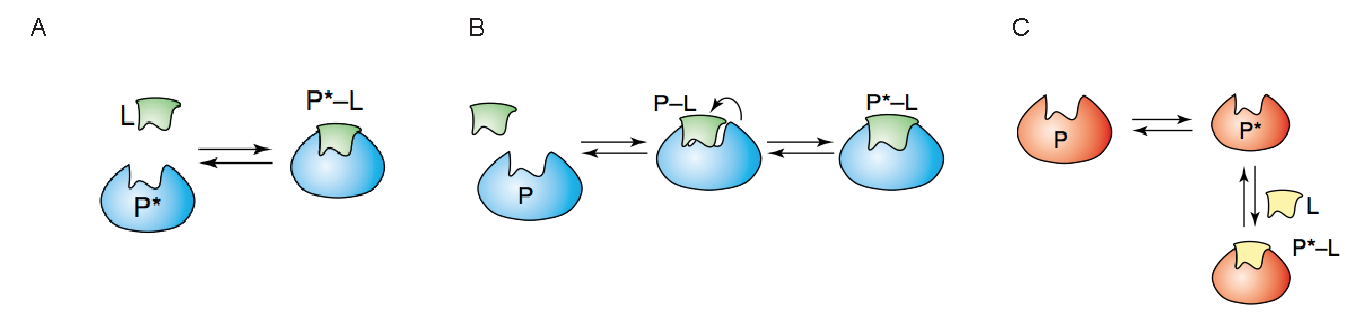
\includegraphics[width=1\textwidth]{images/chap2/figure2_1.pdf} %three modes of binding
   \caption[Three Models of Protein Binding]{ Three models of protein binding. The "lock-and-key" model assumes the protein binding site in a pre-bound state is optimized for the shape of the ligand (A). The "induced-fit" mechanism allows for conformational change after the ligand had bound to optimize shape in a two-step isomerization (B). For the "conformational flexibility" model, the pre-bound structure exists in several isomers which the ligand selects the conformation that compliments it?s structure (C). Figure adapted from \citep{James:2003ts} }
   \label{fig:abmechanism}
\end{figure}


\subsection{Evidence for Conformational Flexibility}
Conformational flexibility is emerging as an important hypothesis to explain both polyspecificity and changes in affinity between germline and mature antibody sequences \citep{Schultz:2002ef,Notkins:2004iz,James:2003ts,Yin:2003wb,James:2003ip,Foote:1994tr,Romesberg:1998ub,Manivel:2000wk,Yin:2001tq,Nair:2002wz,Jimenez:2003by,Li:2003ic,Mohan:2009hs,Marlow:2010jl,Wong:2011ff,Davies:1996wr,Mohan:2003ko,Wedemayer:1997wn,Zimmermann:2010fb}. The first evidence for conformational isomerism in antibodies was observed through kinetic experiments in which antibodies show a triphasic distribution that, in some cases, appears to reflect the existence of multiple isomers of the unbound antibody in solution, in the pre-equilibrium state \citep{James:2003ip}. In 1997, Wedemayer and colleagues found a structural basis for conformational flexibility observed for germline antibodies \citep{Wedemayer:1997wn}. They solved the crystal structures for a germline antibody with and without its target hapten, and an antibody with 6 somatic mutations that bound the target hapten 30,000 times stronger than the germline counterpart. They noticed that the rigid-body deviation in the crystal structure was significant between the bound and unbound germline antibody structure indicating a degree of flexibility. In contrast, the mature antibody had less structural deviation upon hapten binding. They showed that the somatic mutations observed in the mature antibody stabilize the binding sites either directly or indirectly by locking the conformation into place for the pre-bound conformation. This was the first indirect evidence showing that germline sequences may be more flexible than the mature sequences due to the intrinsic properties of the sequence.

More recently, structural studies along with computational tools have corroborated these findings by showing direct evidence that antibodies encoded by germline gene sequences retain flexibility in their HCDR3 loops\citep{Wong:2011ff,Babor:2009it}. For example, Babor et al. redesigned germline or mature HCDR3 loops in antibodies that had been crystallized in free or antigen-bound states\citep{Babor:2009it}. These investigators found that germline gene-encoded HCDR3 sequences are nearly optimal for conformational flexibility. The study, while exceptional in its concept, was limited as the dataset contained many antibody/hapten complexes, which may not reflect the biology of interactions with larger protein targets that are more typical in foreign pathogens. Some antibodies classified as "germline" in the study were not from antigen-na�ve cells. Further, that study exclusively analyzed the HCDR3 loop, not the entire variable region. 

Schmidt et al. used molecular dynamics simulations and structural analysis to determine how mutations in the antibody variable domain enhance antigen binding to influenza HA \citep{Schmidt:2013ka}. In the study, they found two broadly neutralizing antibodies that have branched in lineage from a common intermediate, and an unmutated common ancestor (UCA) in which they obtained high-resolution crystal structures. They found that even though the UCA and mature antibodies have nearly identical binding configurations, the affinity for influenza for the mature antibodies was 40-fold greater than the UCA. Molecular dynamics simulations predicted that the paratope in unbound UCA was not in an optimal conformation for binding, while the mature antibodies had a higher probability of being pre-configured for the influenza HA epitope.

\subsection{Experimental Rationale}
The V\textsubscript{H}-gene encodes the HCDR1 and HCDR2 loops and much of the immunoglobulin framework regions and the beginning of the HCDR3 loop. We hypothesized that the conformational flexibility mediating the polyspecificity of germline gene-encoded antibodies is determined at least in part by the heavy chain variable region encoded by the V\textsubscript{H}-gene, considering it makes up a large portion of the structure. The focus of our study was to test this hypothesis using computational design. Specifically, we analyzed the somatic mutations in sets of mature antibodies that derived from the same V\textsubscript{H} gene and for which co-crystal structures with biologically relevant target proteins were available. Sets of mature antibody-antigen complexes incorporating antibodies that derived from a common germline V\textsubscript{H}-gene were input into the Rosetta "multi-state" design algorithm that recovers the optimal single sequence for an antibody to bind all antigens simultaneously \citep{Babor:2009it,Humphris:2007gq,LeaverFay:2011ji}. The sequences recovered using this protocol would be considered inherently flexible and polyspecific, since they are predicted to accommodate binding to diverse antigens using a structurally diverse set of antibody conformational states. 
In contrast, we also tested monospecificity for each antibody by measuring which sequences are preferred during the design towards a single antigen. This is known as the "single-state" design protocol. For any change between the preference for sequence between the multi-state design protocol that considered polyspecificity and the single-state design that considers monospecificity, recapitulates \textit{in silico}, the process of affinity maturation.

Fundamentally, our approach compares germline and mature antibody sequences optimized in nature through evolution and maturation with sequences predicted to be optimal based on Rosetta's energy function applied to a set of co-crystallized antibody/antigen complexes. The power of the present approach is that we predicted germline and mature sequences \textit{in silico} without any prior knowledge of either, which is an important step towards rational antibody design. We would expect that results of this type of analysis will continue to improve as the size of the collection of conformational ensembles available in the Protein Data Bank (PDB) increases and as the accuracy of the Rosetta energy function continues to improve.

\section{Multi- and Single-State Design of Antigen-Antibody Complexes}
We compiled panels of antigen-antibody complexes from the Protein Data Bank (PDB) in which the antibody heavy chain variable region was encoded by germline V\textsubscript{H}-genes, designated V\textsubscript{H}3-23, V\textsubscript{H}1-69, or V\textsubscript{H}5-51 \citep{Wu:2010dw,Tian:2008vq}. Antigen-antibody complexes were selected only if they contained Homo sapiens or humanized antibodies and the binding partner was a protein antigen. The search of the PDB returns 10, 8 or 3 candidate complexes for V\textsubscript{H}1-69, V\textsubscript{H}3-23, or V\textsubscript{H}5-51 respectively (table \ref{tab:dataset}).
 
\begin{table}[h]
\centering
\begin{tabular}{llllc}
\toprule
PDB ID & V\textsubscript{H}* Germline & Antibody    & Ligand    & V\textsubscript{H}* Mutations \\
\midrule
2CMR   & 1-69*01      & D5          & gp41      & 6             \\
3FKU   & 1-69*01      & F10         & HA        & 13            \\
3GBM   & 1-69*01      & CR6261      & HA        & 15            \\
3MA9   & 1-69*01      & 8066        & gp41      & 4             \\
3MAC   & 1-69*01      & 8062        & gp120     & 7             \\
3P30   & 1-69*01      & 1281        & gp41      & 20            \\
1G9M   & 1-69*02      & 17b         & gp120     & 21            \\
2DD8   & 1-69*05      & M396        & SARS-RBD  & 5             \\
2XRA   & 1-69*05      & HK20        & gp41      & 14            \\
2XTJ   & 1-69*10      & 1D05        & PCSK9     & 4             \\
2QQN   & 3-23*01      & anti-Nrps-1 & Nrps-1    & 10            \\
2R56   & 3-23*01      & IgE         & BLG       & 23            \\
2VYR   & 3-23*01      & VH9         & MDM4      & 10            \\
3KR3   & 3-23*01      & DX-2647     & IGF-II    & 8             \\
1S78   & 3-23*04      & Pertiuzimab & ErbB2     & 22            \\
2FJG   & 3-23*04      & G6          & VEGF      & 15            \\
3DVN   & 3-23*04      & Apu2.16     & Ubiquitin & 18            \\
3BN9   & 3-23*04      & E2          & MT-SP1    & 5             \\
2B1A   & 5-51*01      & 2219        & UG1033    & 17            \\
2XWT   & 5-51*01      & K1-70       & TSHR      & 8             \\
3HMX   & 5-51*01      & Ustekinumab & IL-12     & 12           \\
\bottomrule
\end{tabular}
\caption[Antibody-Antigen Test Set]{Antibody-antigen test set. Details of the 10, 8, and 3 complexes for V\textsubscript{H}1-69, V\textsubscript{H}3-23, and V\textsubscript{H} 5-51 respectively. The antibodies bind a diverse set of antigens but each share a common germline across a test set. The V\textsubscript{H} mutation count of amino acid mutations away from their inferred germline gene. *Predicted from IMGT}
\label{tab:dataset}
\end{table}


 
For each panel we compared the mature (somatically mutated) sequence to the inferred germline gene sequence via a multiple sequence alignment (figure \ref{fig:polymethods}A). The number of mutations with respect to the germline sequence range from 4 to 23 mutations with an average of 12.2. All HCDR1, HCDR2, and framework positions that differed from the germline sequence of the common V\textsubscript{H}-gene sequence in at least one position in the multiple sequence alignment were included in the computational design simulations as "variable positions". Note that our study explicitly excluded positions that remained unchanged as no claims can be made with respect to the relevance of these positions for conformational flexibility or polyspecificity. Our analysis is limited to antibody regions encoded by the V\textsubscript{H}-gene as only this region can be unambiguously aligned within each set of antibodies. Therefore, we excluded D-gene and J-gene that encode HCDRH3, and antibody light chain positions. The identity and conformation in all variable positions to identify the sequence and conformation that return minimal energy for the given protein backbone of the antibody/antigen complex \citep{Kuhlman:2000tc}. In this work, we used multi-state design\citep{LeaverFay:2011ji} to find a single sequence that minimized energy with all antigens within each V\textsubscript{H} gene-encoded group. To reduce noise in the outcome of the computations, 100 simulations were executed, and results are displayed using WebLogo representation \citep{Crooks:2004do} (figure \ref{fig:polymethods}C). 

For a concrete example, consider position 31 (PDB numbering, boxed in \ref{fig:polymethods}C). This position, encoded by V\textsubscript{H}5-51, diverged from a germline serine residue in the sequence for all three complexes. Complexes 2B1A and 2XWT (PDB code) possess an aspartate residue in this position acquired by somatic mutation, while 3HMX has a threonine in the same position. The multi-state design protocol selected the germline residue serine as the energetically most favorable residue out of all 20 possible genetically encoded amino acids when interaction with all three structurally diverse antigens is required. The experiment was repeated as three separate "single-state design" experiments (figure \ref{fig:polymethods}B, right side) to predict the sequences and conformations that minimized interaction energy for each antigen individually. The resulting sequences were compared to both the inferred germline and the mature sequence (figure \ref{fig:polymethods}C). In this experiment position 31 is predicted as an aspartate for complexes 2B1A and 2XWT, and as a threonine for 3HMX, the mature amino acid sequence (data not shown).

For this work, it was important to convert the outcome to a statistical quantitative analysis. Each design outcome is compared to the mature or germline sequence, by computing a bit-score "recovery" measure. The results can either recover towards germline, mature or neither sequences. The bit-score computation we used is described in the methods of the appendix section. The advantage of the bit-score measure in comparison to a more simplistic percentage-recovery is that it analyzes the relative probabilities of all twenty amino acids in a particular sequence position, not just the probability of the correct one. It thereby arrives at an accurate measure of "surprise" of seeing a certain outcome, a normalized measure in information theory that can be readily compared between different experiments. In our experiment high bit-score for the germline sequence indicated that among the 100 designed sequences, germline gene-encoded residues were chosen in a large number of instances (figure \ref{fig:polymethods}D). To facilitate comparison across complexes that have a different number of designed entities considered, we determined the sum bit-scores over all designed positions and normalized the score to fall between 0 and 1 by division with the maximum bit-score that could be achieved, i.e., every amino acid position designed towards a germline or mature sequence. 

\begin{figure}
\centering
 \includegraphics[scale=.5]{images/chap2/figure2_2.pdf}
   \caption[Multi-State and Single-State Design Methodology]{Multi-state and single-state design methodology. For a simplified view of the methodology, only the complexes from inferred germline V\textsubscript{H}5-51 are presented. The heavy chain variable segment amino acid sequences taken from the PDB were aligned.  Position candidates were chosen for design if the position differed from the germline sequence in at least one mature complex (A). Co-crystal structures for each V\textsubscript{H}5-51 derived complex are shown with heavy chain in black, light chain in grey, antigen in magenta, and designed positions highlighted in gold. Single- and multi-state design schemes are shown where each complex was designed alone (single-state) where the designed positions were optimized to minimize the energy for a single antigen target, or a minimized energy for all complexes considered together (multi-state) where the sequence returned was an energetic consensus among each complex considered (B). Sequence logos were generated to show 100 design models. Each position in the sequence logo corresponds to a position conserved for design.  The sequence logos then were compared to the mature or germline sequence for each antibody (C). Bit-scores were determined quantitatively by measuring the frequency of a letter at each position. The bit-score measures the designed residues compared to either the germline sequence or the mature sequence. The normalization factor was the [total bit-score]/[perfect design score] (D).}
  \label{fig:polymethods}
\end{figure}


\section{Specificity Inferred by Sequence Design}
The results of the multi-state design simulations returned sequences that resembled germline gene-encoded sequences more often than mature sequences. This finding was remarkable as no information about germline sequences was input into the simulation. We found that the designed sequences gave normalized bit-scores of 0.54, 0.60, and 0.43 for germline genes V\textsubscript{H}1-69, V\textsubscript{H}3-23, or V\textsubscript{H}5-51, respectively. In contrast, statistically significant reduced bit-scores of 0.48, 0.45, or 0.26 (p < 0.0001) were observed when comparing the designed sequences with the mature genes (figure \ref{fig:polyresults}A).
The single-state redesign of mature antibodies for binding to their associated antigen gave normalized bit-scores of 0.47, 0.43, or 0.28 for comparison with germline gene-encoded sequences and 0.57, 0.54, or 0.53 for comparison with mature sequences of V\textsubscript{H}1-69, V\textsubscript{H}3-23 or V\textsubscript{H}5-51, respectively. In this design experiment, a proclivity to recover the somatically mutated mature sequences was observed (figure \ref{fig:polyresults}A). Given that a normalized bit-score is the preference for each design experiment to match a certain sequence profile, a high bit-score to germline sequence indicates the output matching the germline profile, while a high bit-score to the mature sequence indicates a preference for the mature profile, each design experiment outcome can be measured as a difference in bit-scores (mature - germline). With this definition, a preference for mature sequence gave a positive $\Delta$bit-score, while a preference for germline residues gave a negative $\Delta$bit-score for a given complex - i.e., the $\Delta$bit-score provided an \textit{in silico} predicted metric for antibody optimization for affinity to a specific antigen versus polyspecificty. We observed positive values for single-state design and negative values for multi-state design, indicating a preference for the mature or germline sequences, respectively (figure \ref{fig:polyresults}B, p < 0.0001).

\begin{SCfigure}
   \centering
   \caption[Multi-State Designs Toward the Germline Sequence ]{Multi-state designs toward the germline sequence. Antibodies encoded by the same inferred germline V\textsubscript{H} gene preferred germline sequences when considered in the multi-state design, inferring a more flexible combining site. The bar graph shows the bit-score for each of the three different inferred germline groups and then the sum of the scores in a grouped bar. A perfect design would have a normalized bit-score of 1.0, and summated score of 3.0 for three germline groups. Multi-state design preferred germline sequences for all complexes, while in contrast single-state design preferred mature sequences (A, p<0.0001). The change in bit-score is determined to be the proclivity to either the mature (positive score) or the germline (negative score) sequence. Each complex was assigned a change in bit-score. The change in proclivity between design protocols was significant (B, p< 0.0001). Each complex was scored against mature and germline sequences and a difference was calculated ($\Delta$bit-score). Positive numbers returned showed a proclivity towards mature sequences, while a negative score suggested a design toward germline. A tight correlation was observed (r$^{2}$=0.8263) for the \textit{in silico} predicted optimization for specificity versus polyspecificity ($\Delta$bit-score) and the \textit{in vivo} maturation process (C, plotted as the mutation percentage away from V\textsubscript{H} gene sequence).}
   	\includegraphics{images/chap2/figure2_3.pdf}
   \label{fig:polyresults}
\end{SCfigure}


\section{Affinity Maturation Correlates with Predicted Affinity}
The number of somatic mutations can be used as a measure of the maturity of an antibody \citep{Briney:2012ib}. Hence, we asked the question if the $\Delta$bit-score, the change in proclivity for a germline or mature sequence, correlated with affinity, i.e., if tendency to recover mature versus germline sequences increased as antibody maturation progressed. Such a correlation would indicate that as antibodies mature, features of the germline sequence critical for polyspecificity are replaced with features critical to recognize one target antigen. Figure \ref{fig:polyresults}C shows the somatic mutation percentage of antibodies in each complex as a metric  for ?\textit{in vivo} maturation? correlated with the $\Delta$bit-score as a metric for "\textit{in silico} predicted optimization for affinity versus polyspecificty". For positive $\Delta$bit-scores, the mature sequence was preferred, indicating a preference for specificity. For negative values, the germline sequence, and hence polyspecificity was preferred. The correlation coefficient for the "\textit{in vivo} affinity maturation" and "\textit{in silico} predicted optimization for affinity vs. polyspecificity" was 0.83. 

\section{Backbone Conformational Space for Germline Sequences}
Torsional phi-psi angles in the protein backbone were compared across the sets of experimental structures for positions that recovered to germline sequence for multi-state design and those positions that recovered to a non-germline sequence.   We found that positions that converted back to germline in multi-state design, i.e., positions critical for conformational flexibility according to the simulation, had a deviation of 19.6$^\circ$ $\pm$ 2.0$^\circ$ across beta-sheet phi-psi torsion angles. Sequence positions that did not recover to a germline gene-encoded amino acid had a statistically significant (p = 0.099) reduced deviation of 15.5$^\circ$ $\pm$ 1.5$^\circ$ for beta-sheet backbone torsion angles (figure \ref{fig:polyfw}A-C). Considering the limited range for beta-sheet backbone torsion angles, we don't expect large deviations. For reference, all framework residue beta-sheets in antibody-antigen complexes across our dataset have an average phi-psi deviation of 18.7$^\circ$ $\pm$ 0.9$^\circ$.  

\begin{SCfigure}
   \centering
   \caption[Phi-Psi Variances for Framework Residues]{Phi-psi variances for framework residues. The degree of structural variation of the framework residues were measured as the standard deviation of the phi and psi angles over each residue position. Side view of immunoglobulin fold for V\textsubscript{H}5-51 complexes aligned by framework residues. Beta-sheets included in the analysis are shown as a cartoon representation, while loop regions are in a transparent ribbon representation. Framework 1 is shown in brown, HCDR1 in green, framework 2 in black, HCDR 2 in magenta, and framework 3 in cyan (A). Same as (A) but top down view (B). The standard deviations of the phi-psi angles of each framework position were binned into either a residue that was found to be critical for polyspecificity (recovered to germline) or a residue that was not recovered to germline in multi-state design.  For each position, the phi-psi angles were averaged, and the standard error of the mean was calculated. An average of 19.6$^\circ$ $\pm$ 2.0$^\circ$ for germline recovered residues and 15.47$^\circ$ $\pm$ 1.5$^\circ$ for non-germline recovered residues supporting our hypothesis that residues which enable polyspecificity alter beta-sheet packing to a greater degree than residues that do not. The axis is normalized to 18.7$^\circ$ $\pm$ 0.9$^\circ$, the average deviation for all beta-sheet framework positions (C).}
   	\includegraphics{images/chap2/figure2_4.pdf}
   \label{fig:polyfw}
\end{SCfigure}


\section{Impact of Residue Environment on Specificity}
Figure \ref{fig:polyenv} maps each amino acid position encoded by the V\textsubscript{H} gene segment onto the immunoglobulin fold using a custom Collier de Perles representation, as described by Ruiz and Lefranc\citep{Ruiz:2002jd}. We modified the output to distinguish positions by location in the interface with the antigen and the degree of burial. We correlated these metrics to the bit-score at a per-residue level. Each residue given is in IMGT numbering.

For multi-state design (figure \ref{fig:polyenv}A-C), 33 out of a possible 46 of the designed interface residues (72\%) contributed to polyspecificity, i.e., recovered to germline sequence with a normalized bit-score > 0. Remarkably, also 41 out of 77 residues outside the interface (53\%) recovered to germline. Residues 25, 40 and 105, far removed from the interface, recovered perfectly (normalized bit-score = 1) in at least two of the three germline gene test sets. These residues are highly buried, with a neighbor count score of 13.3 $\pm$ 0.5. The intermediately packed residues 17, 51, 70, and 71, with an average neighbor score of 8.6 $\pm$ 2.2 neighbors, were predicted to contribute to polyspecificity, even though they lie in distal positions from the antigen-binding site. The interface residues 35, 63, 64, and 82 were found to contribute to polyspecificity in two out of the three germline gene test sets. A conserved serine, which was found in all three germline sequences at position 36 in the CDR1, was the only residue identified as critical for polyspecificity in all three germline genes. 

In contrast, for single-state design, it is more difficult to deduce overall trends for any specific position as the paratope is altered in each antibody and the recognized epitopes cover diverse structural space. Generally, when each complex was considered individually, 214 designed interface residues recovered to their mature sequence out of a possible 340 designed amino acids, indicating their importance for recognition of, and affinity for binding to, the specific antigen (63\%, figure \ref{fig:polyenv}D-F). When non-interface residues were considered, 411 out of a possible 699 designed residues recovered to their mature sequence (59\%). away from residues encoded by their inferred germline gene. Of these mutations, 68 out of 110 interface residues recovered to the mature sequence (62\%) in single-state design, while 72 out of 145 non-interface residues recovered to the mature sequence (49\%).

Residues that were found to be critical for polyspecificity, i.e., reverted to germline in multi-state design, differed substantially for each germline gene test set considered. For the V\textsubscript{H}1-69 gene derived antibodies, all of the residues in the HCDR2 loop contributed to binding interactions in the single-state but not the multi-state design. In contrast only G63 and T64 residues contributed in the multi-state case but not in single-state designs. Residue L50 was recovered in all single-state complexes but was not critical for multi-state design. For the V\textsubscript{H}3-23 gene, residues A55 and Y66 were not recovered in multi-state design but were found to be important for high affinity in single-state design. For the V\textsubscript{H}5-51 complexes, non-interface residues P15, M53 and A80 were not recovered in multi-state design but were found to be critical in single-state design. HCDR2 was found to be critical in single-state design for all V\textsubscript{H}5-51 complexes.

\begin{figure}
\centering
 \includegraphics[scale=.6]{images/chap2/figure2_5.pdf}
   \caption[Colliers de Perles Representation of V\textsubscript{H} Gene Segments ]{Colliers de Perles reepresentation of V\textsubscript{H} gene segments. The 98 amino acids present in V\textsubscript{H}1-69, V\textsubscript{H}3-23, or V\textsubscript{H}5-51 are shown in a Collier de Perles two-dimensional representation and numbered according to the IMGT numbering scheme 37. Hatched circles are missing residues according to the IMGT numbering scheme and are shown to make graphs consistent. Square boxes represent the boundary between framework and CDR loops. The anti-parallel beta-sheets are represented A-F.  A dashed line is shown that divides interface residues with residues that were found to be outside of the interface in a majority of the cases. Interface residues are colored with a blue-pink gradient indicating a numerical antigen contact score defined by a change in neighbors between the free and bound complex. Non-interface residues are colored with a green-orange gradient according to their degree of burial defined through a neighbor count. Residues that are transparent were not considered for redesign as they were conserved across all complexes considered. (A, B, C) show the germline sequence represented in the immunoglobulin fold with the thickness of each line representing the design bit-score for that position relative to the germline sequence for multi-state design protocols for V\textsubscript{H}1-69, V\textsubscript{H}3-23, or V\textsubscript{H}5-51, respectively. (D, E, F) show the germline sequence represented, but the thickness of the line corresponds to the mature sequence bit-score averaged over each complex for the single-state design protocol for V\textsubscript{H}1-69, V\textsubscript{H}3-23, or V\textsubscript{H}5-51, respectively.}
  \label{fig:polyenv}
\end{figure}


\section{Mature Sequence Bias}
To understand some of the trends described above more quantitatively, we determined for each residue in each antibody/antigen complex if it was part of the interface, i.e., directly engaging the antigen. For this purpose the change in neighbor count between unbound antibody and bound antibody/antigen complex score was measured, and positions with a change larger than 1.0 were classified as "interacting residues". Next, we counted how often a residue position appeared in the interface within each set of antibody/antigen complexes. Positions were binned as occurring in the ensemble interface never, once, two-four times, or more than four times and average bit-scores were compared (figure \ref{fig:polymsb}). We found a general trend for interface ensemble size correlating with interface ensembles sampled. For the set of structures derived from V\textsubscript{H}3-23, which contained a total of 8 complexes, we found that residue positions that are never found in the interface gave an average bit-score of 2.3 $\pm$ 0.4. If a residue position was found only in one interface, the average bit-score dropped to 1.2 $\pm$ 1.1. As residues were found more frequently at the interface between 2-4 complexes, and 5-8 complexes, the average bit-score increased to 2.5 $\pm$ 0.8 and 3.6 $\pm$ 0.7 respectively. For the 10 V\textsubscript{H}1-69 complexes, an average bit-score of 2.3 $\pm$ 0.3 was observed for residues that were never found in the interface. If a residue was only found in the interface once, the average bit-score dropped to 1.9 $\pm$ 1.0. For interface occurrences between 2-4 and 5-8, we found the average bit-score to increase to 2.6 $\pm$ 0.7 and drop to 0.8 $\pm$ 0.4 respectively. Due to the limited number of residues occurring in multiple interfaces, a significant change in bit-score between each grouping was not observed for V\textsubscript{H}1-69 (p= 0.1844) and V\textsubscript{H}3-23 residue positions (p=0.2007). 

\begin{figure}
   \centering
   \includegraphics{images/chap2/figure2_6.pdf}
   \caption[Interface Occurrences Affect Germline Sequence Recovery]{Interface occurrences affect germline sequence recovery. For V\textsubscript{H}3-23 (A) and V\textsubscript{H}1-69 complexes (B), we binned each residue position into how many times it occurred in an interface (interface ensembles). Most designed positions never occurred in an interface. As their occurrences became more frequent, we observed a trend for increasing the recovered germline residue. This trend fell off for V\textsubscript{H}1-69 complexes (B) for positional occurrences between 5-8 interfaces.}
   	   \label{fig:polymsb}
\end{figure}


\section{Evolutionary Sequence Bias}
We expected the result of multi-state design to deviate from germline in cases where alternate amino acids are compatible with the conformational space and binding modes observed in the ensemble of structures. Alternative amino acids might be tolerated but are not observed in evolution - "evolutionary sequence bias". To test this hypothesis, we reverted each position back to germline and compared the energetic change with the favored residue returned by multi-state design. Using reference energies, Rosetta facilitates the direct comparison for energies between different residue types \citep{Kuhlman:2003kp}. For complexes derived from V\textsubscript{H}5-51, all positions in which the germline residue were not chosen in at least 10\% of the 100 simulated models were forced into the germline identity (Figure \ref{fig:polyesb}A, x-axis). The difference in average energy of the germline sequence at that position from the average energy of the residue returned by multi-state design was calculated (y-axis). For each position, if positive values were returned for all three complexes, RosettaDesign would most likely place a non-germline amino acid at that position. If negative values were returned for all three complexes, Rosetta would most likely place a germline amino acid at that position. We found that, in most cases, the energetic contribution of the designed amino acid is not significantly more stabilizing than the germline amino acid, i.e. the germline sequence is tolerated as well. Only positions 52, 76, 88, and 98 gave a significant energy increase for the germline sequence in at least one complex. Changes in energy were classified as significant if larger than 0.7 Rosetta energy units (REU, horizontal dashed line). This threshold was derived from the average difference in energy between the germline and mature residue (0.7 $\pm$ 0.2 REU, data not shown). For Figure \ref{fig:polyesb}B, a multiple sequence alignment is given as a reference, where each position that was considered in multi-state design is highlighted in bold while each position that recovered well to the germline sequence is highlighted in green. 

\begin{figure}[t]
   \centering
   \includegraphics[width=.9\textwidth]{images/chap2/figure2_7.pdf}
   \caption[Rosetta Multi-State Design Solutions]{Rosetta multi-state design solutions. We evaluated a complete germline reversion of V\textsubscript{H}5-51 sequence versus the sequences output by multi-state design. (A) Consideration of positions in which the multi-state design algorithm chose a non-germline amino acid for at least 10\% of the models where evaluated. The difference in energy of the germline sequence and the multi-state design solution sequence is shown for each position. Bars above 0 represent the multi-state design sequence preferred while bars below the line represent the germline amino acid preference. The horizontal dashed line at 0.7 Rosetta energy units (REU) shows the average energy difference between the germline and mature sequence and is represented as a marker for sequence tolerance. (B) The multiple sequence alignment for each V\textsubscript{H}5-51 complex is shown and compared with the germline sequence. Sequences highlighted in bold were considered for design. Sequences highlighted in green are positions in which the multi-state design algorithm chose the germline amino acid as the design solution. The numbers in the bottom row are the alignment-numbering scheme of each position and correspond to the position numbers in (A).}
   	   \label{fig:polyesb}
\end{figure}



\section{Discussion}
\subsection{Limitations of Computation}
We recognize several important limitations of our study: \begin{enumerate}
\item We assumed that the RosettaDesign protocol determined the optimal sequence for any given design challenge. While it has been demonstrated that RosettaDesign typically recovers close-to-optimal sequences \citep{Kuhlman:2000tc}, inaccuracies in the scoring function and limitations in the sampling algorithm will introduce errors. In the future, this limitation could be reduced by improvements applied to the energy function and comparing the results obtained with complementary energy functions. We assumed that the finite and small set of antibody conformations observed in the set of co-crystallized mature antibodies completely describes the conformational flexibility of the germline gene-encoded antibody (finite ensemble bias). While we used the largest ensembles available (10, 8, and 3 antigen-antibody complexes), this assumption must be wrong, introducing a bias. For example, assume there is a sequence position that is part of the paratope in only one of the n complexes. In this antibody, a somatic mutation occurred at this position greatly increasing affinity to the antigen. The somatically mutated amino acid is however compatible with all other n-1 complex structures. In such a scenario the multi-state design algorithm will recover the somatically mutated instead of the germline amino acid. Here, we found that as a residue was more often part of the paratope, it became more likely to be recovered to the germline sequence. This finding might be due to the fact that a critical conformation that the germline antibody needs to adopt was not represented in the ensemble (for framework residues) or the epitope needed for recognition by a critical germline amino acid represented in the ensemble.

\item We assumed that the germline gene-encoded antibodies were able to adopt the conformations of each of the mature antibodies derived from it. This assumption is important, as crystal structures of the "true" germline antibody in complex with the antigen are generally not available. While this assumption is expected to be correct for the majority of cases, notable exceptions are discussed in the literature \citep{Yin:2003wb,Li:2003ic,Wedemayer:1997wn,Sethi:2006dq}. 

\item It is not guaranteed that only the germline amino acid is compatible with all conformations adopted by mature antibodies. Rather, it is likely that for some positions alternative amino acids are plausible or even better in realizing the conformational flexibility needed. The germline sequence observed in nature is optimized in evolution and clearly works, but does not need to be perfect in all positions. In such a scenario, multi-state design could return amino acids that deviate from germline (evolutionary sequence bias). Conversely, the mature sequences observed in the co-crystal structures are not guaranteed to be the perfect sequence for high affinity. In some positions a somatic mutation might have introduced a better amino acid but is not the "true" best option. Some somatic mutations might have occurred by chance and do not contribute to affinity maturation. Some positions might not have experienced somatic mutations but still favorable mutations exist. In all these cases we expect the single-state design to deviate from the mature sequence observed in the co-crystal structure (evolutionary sequence bias).

\item The imperfect nature of the Rosetta scoring function will not yield 100\% agreement with natural phenomenon \citep{Kuhlman:2000tc}. Importantly, water coordination can often be important in antibody-antigen binding sites38. However, Rosetta is currently being developed to include tools with explicit solvent models \citep{Lemmon:2012ku}.



\end{enumerate}
It is important to understand these biases and limitations to arrive at an accurate interpretation of the results. Given these known limitations, we expected imperfect agreement of \textit{in silico} predicted and natively observed mature and germline gene-encoded antibody sequences. Nevertheless, we found a remarkably high correspondence of residues designed for polyspecificity in a blinded fashion and the amino acids encoded by germline genes.

\subsection{Interpretation}
Germline gene-encoded sequences for commonly used V\textsubscript{H} segments are hypothesized to possess high conformational flexibility making them ideal for binding diverse antigens, i.e., being polyspecific. During antibody maturation, somatic mutations are introduced that increase affinity for a specific target in part by adding attractive interaction to the antigen (increasing enthalpic gain) and in part by locking the conformation critical for interaction with the specific antigen (reducing entropic cost). Here we tested this hypothesis by analyzing three sets of antibodies, each derived from a commonly used V\textsubscript{H} gene and each co-crystallized with a protein target in its antigen-specific binding conformation. 

We chose to not directly compare conformational flexibility for germline and mature antibodies. While this approach may be feasible in general through predicting the accessible conformational space using molecular dynamics \citep{Wong:2011ff}, it is challenging to achieve complete sampling of large conformational spaces that include the entire immunoglobulin framework. To circumvent this problem, we chose to solve the inversely related protein design problem, which was to study amino acid sequences that are consistent with the conformational space seen in antibody/antigen co-crystal structures. This approach is complementary and potentially superior as it replaces sampling of the large conformational space in antibody backbone regions with solving the better understood ranking of amino acid sequences, given a certain antibody/antigen complex conformation. Specifically, we employed multi-state design to find single amino acid sequences that were compatible with the multiple conformations of antigen combining sites. 

Computational tools to design multi-specific proteins were first described by pioneering work in the Kortemme laboratory\citep{Babor:2009it,Humphris:2007gq}. In parallel, Leaver-Fay and colleagues developed a general algorithm for multi-state design in the Rosetta framework, in which they designed one protein to interact with non-native targets\citep{LeaverFay:2011ji}. We used the latter tool to design antibody sequences that are optimal for facilitating interactions to \begin{enumerate}
\item multiple and diverse antigens, or
\item a single specific antigen. 
\end{enumerate}

In the absence of a priori knowledge of the germline or mature sequences or the mechanism of antibody maturation through somatic mutations, multi-state design of one antibody to recognize several target proteins recovered sequences similar to those encoded by the inferred germline gene segment. When designing the same antibody to recognize one specific target, the sequence recapitulated the mature antibody sequence. This trend correlated tightly with the divergence of the mature sequence from the inferred germline sequence, i.e., the more somatic mutations an antibody contained, the more reversions to germline needed in order to facilitate interactions to multiple antigens.

Use of a computational tool to approach questions regarding polyspecificity as a function of protein sequence is advantageous, as the RosettaDesign algorithm is able to rapidly enumerate the effect of multiple simultaneous mutations in sequence space for the entire heavy chain variable region. This task is quite difficult if not impossible to complete experimentally at this scale. In this manner, conformational flexibility in the framework regions, HCDR1, and HCDR2 can be tested in a holistic model. All mutated positions in the V\textsubscript{H} gene segment were considered simultaneously, including the effect of interactions between different domains in the antibody, thus revealing the role of interface and non-interface residues in both poly- and monospecificity. Because this approach considers multiple antibodies of variable conformation at once, each with a distinct binding mode, the multi-state design algorithm predicts sequences that are inherently flexible and capable of adopting the diverse set of conformations needed to bind to multiple antigens.
 
Harindranath and colleagues demonstrated that polyspecific antibodies were encoded largely by germline gene sequences \citep{Harindranath:1993ty}. Romesberg and Spiller presented structural evidence for flexibility in germline gene-encoded sequences \citep{Romesberg:1998ub}. In addition, Schmidt et al. correlated mature sequence to rigidity of the paratope \citep{Schmidt:2013ka}. Taken together, these data suggest conformational flexibility coupled with pre-sampled conformations of the target binding site as the underlying mechanism for polyspecificity \citep{Wedemayer:1997wn}. Here, we used a multi-state design algorithm to assess the contribution of the V\textsubscript{H} gene segment to specifying an antibody with conformational flexibility, preorganization, and polyspecificity. We found that this property is largely attributed to antibody sequences in the germline gene repertoire, since designing antibodies for polyspecificity, sequences recovered germline gene-encoded sequences, while designing antibodies for monospecificity to a single target, returned sequences similar to the mature antibody. This trend increased in strength the higher the number of somatic mutations that had accumulated, i.e., the further optimized the antibody had become. Importantly, this effect is not limited to the HCDR3, which often contributes much to antibody specificity. We obtained the same finding to be clearly measurable throughout HCDRs 1 and 2 as well as the immunoglobulin frameworks. We found each germline V\textsubscript{H} gene to encode a set of amino acids that enabled polyspecificity in a distinct manner. These positions were present not only in the paratope, but also in the buried or semi-buried positions of the immunoglobulin frameworks (figure \ref{fig:polyenv}). We expect, that with an increasing number of antibody-antigen complexes in the PDB it will become easier to discern general trends. 
 
We conclude that conformational flexibility in the beta-sheet framework is critical for changing critical regulators of the conformation of the paratope - i.e., the takeoff and landing angles of HCDR loops, thereby enabling the paratope of germline antibodies to assume multiple conformations. Accordingly, we find that residues that contribute the most to polyspecificity contain larger deviations of their phi-psi torsion angles (figure \ref{fig:polyfw}). During antibody maturation, mutations in these positions likely lock in the target-specific framework conformation, reducing the entropic cost of target binding. Somatic mutations in the paratope, for example within HCDR1 and HCDR2, can directly increase affinity to a target (enthalpic contribution to free energy), or lock in a conformation that recognizes the target (entropic contribution to free energy). We found that on average 62\% of residues in the paratope and 42\% of residues in the framework were important for changing the binding pattern of the antibody from polyspecificity to recognition of one specific target (figure \ref{fig:polyenv}). 
 
We identified at least four specific scenarios in which current datasets are limiting for informing design efforts:
\begin{description}

\item[The first scenario] involves a framework position that does not interact with the epitope in any of our tested complexes. For this position, the germline residue, and only the germline residue, is capable of adopting the phi-psi angles in order to accommodate the flexibility needed for the binding site. Multi-state design likely designs in the germline residue for each simulation. We then observe agreement between \textit{in silico} design and natively observed sequence for a majority of the designed positions (figure \ref{fig:polyresults}). 

\item[The second scenario] involves a framework position that also lies distal from the epitope. In this scenario, the germline residue but also other amino acids are compatible with the observed conformations since they both contain properties to adopt the phi-psi angles necessary to accommodate the flexible binding site. For this scenario, we expect Rosetta?s multi-state design algorithm to pick one of the compatible amino acids, not necessarily the germline gene-encoded one. This outcome can occur either because the conformational ensemble is incomplete or because of the evolutionary sequence bias. We find that both biases contribute to ambiguity. Residues that are never found in the interface give modest recovery to germline sequences being either "hit-or-miss" (finite ensemble bias, figure \ref{fig:polymsb}), and residues that are reverted to an amino acid different from that encoded in the germline are not significantly better in energy score than the germline encoded amino acid (evolutionary sequence bias, figure \ref{fig:polyesb})

\item[The third scenario] concerns residues that are at part of the paratope in only one instance. If the mature residue forms critical interactions that minimize the free energy of binding in this one complex, while in all other complexes the residue is not part of the paratope and the mature amino acid seen for the one complex is compatible with the backbone confirmation, Rosetta will choose the mature residues from the first complex also in multi-state design mode. We observed this trend, especially for V\textsubscript{H}3-23 complexes. If a residue was found in only one interface (figure \ref{fig:polymsb}), that position tended to have a low recovery to the germline sequence. 

\item[The last scenario] deals with positions that are part of the paratope multiple times and that experience frequent somatic mutations. As positions are found to be more frequently in interface ensembles, the germline recovery increases as these positions become more important to facilitating direct interactions with their antigen (figure \ref{fig:polymsb}). These residues contribute to polyspecificity by being the preferred residue in interaction with multiple antigens, rather than facilitating binding by altering beta-sheet packing.
\end{description}

\section{Conclusions and Future Directions}
These results suggest that the naturally occurring antibody maturation process can be recapitulated or reversed at least partially \textit{in silico}, opening exciting new avenues for antibody engineering work. Further, our results suggest the applicability of multi-state design to engineer polyspecific antibodies, exploring another important strategy for designing broadly neutralizing antibody therapeutics. Traditional antibody engineering approaches emphasize isolating monoclonal antibodies that are highly specific for a given antigen, relying on display techniques in which emphasis typically is placed only on HCDR loop design. The method described here considers the entire antibody variable region during design, including critical framework residues that allow for conformational flexibility and contribute to polyspecificity. Considering that we found that up to 64\% of framework and HCDR residues may contribute to binding and specificity, computational design will be invaluable to rapidly enumerate the large sequence and structural space of residues that can contribute to breadth of binding diverse targets. 



%\chapter{HIV Neutralizing Antibodies in HIV Na\"{i}ve Donors}
\section{Introduction}
The induction of broadly neutralizing HIV-specific antibodies is likely to be a critical component of the mechanisms of protection for an effective HIV vaccine. In the work presented here, we used a novel approach for examining the heavy chain complimentary determining region 3 (HCDR3) repertoire of HIV-naïve donors to interrogate the structural properties of long HCDR3 loops. Some broadly neutralizing HIV-neutralizing human antibodies possess long HCDR3 regions, which typically are created at the time of original antibody gene recombination rather than during somatic hypermutation. We sought to determine if antibodies with long, structured HCDR3s that are present in the naïve B-cell repertoire of HIV-naïve donors confer neutralizing properties to those antibodies similar to that of previously isolated HIV-neutralizing antibodies such as PG9 and PG16, which target the HIV envelope protein variable loops 1 and 2. Using ultra-deep nucleotide sequence analysis of HCDR3 regions in antibody gene replicons for 64 different HIV-naïve donors, we obtained approximately 25,000 unique sequences that encoded HCDR3s of 30 amino acids in length. The modeling suite Rosetta was used to assess the ability of these 30 amino acid length HCDR3 sequences to form a loop with structure similar that of antibody PG9. The PG9 backbone template then was threaded rapidly with sequences from HIV-naïve donors to evaluate the energetic state of naturally occurring long HCDR3s when tested in a PG9-like conformation. The sequences encoding HCDR3s with the most favorable predicted energy states in this conformation then were redesigned in silico to optimize binding with minimal changes, simulating the process of somatic hypermutation. The sequences that were found to mimic the binding energy and HCDR3 structure of PG9 were synthesized and characterized experimentally for ability to bind to HIV envelope (env) protein and neutralize HIV infectious virions. We find 12 unique antibodies that present PG9 HCDR3 mimicry with 0 to 7 mutations away from their respective HIV-naïve wild-type sequence. This work, using a robust new bioinformatics and modeling pipeline, suggests that HIV-naïve donors may possess naïve B-cells encoding antibodies with long HCDR3s that can neutralize HIV prior to infection. Expanding and preserving these unique naïve B-cells from the naïve repertoire may represent an important new strategy for HIV vaccine priming.

\subsection{Potential Paradigm Shifts in Vaccinology}
Elicitation of broadly neutralizing antibodies (bNAbs) against human immunodeficiency virus type 1 (HIV-1) has been one of the greatest challenges in modern vaccinology1,2. A bNAb response occurs in 10-30\% of those infected, with about 1\% of those possessing ‘elite neutralization’ breadth3. These antibodies typically arise 1 year after infection at the earliest and peak at approximately 3-4 years after infection4. Recent advances in donor selection from cohorts of chronically infected patients, novel screening methods, and antibody isolation technologies, have allowed identification of dozens of new antibodies to the envelope protein gp120/gp41 of HIV-15. These antibodies bind at least five major epitopes on gp120 including the CD4 binding site6, the gp120 outer domain7,  the V3 loop and V3 complex glycans8, the V1/V2 loop and surrounding glycans9, or the membrane proximal region (MPER) on gp4110. While the various bNAbs of interest were isolated using different strategies, they often share certain unusual and distinctive genetic features, such as very large numbers of somatic mutations or very long non-canonical heavy chain complimentary determining region 3 (HCDR3) structures11.

Although studies based on bNAb isolation have revealed new targets for immunogen design and have been useful for experimental therapeutic efficacy12, the design of a vaccine against HIV-1 that induces sterilizing or protective immunity has remained elusive13. For example, the RV144 trial that tested a vaccine strategy using priming immunization with a recombinant canarypox vector followed by a bivalent gp120 protein boosting immunization revealed 31\% efficacy and 60\% efficacy in the first year for this regimen14. While the RV144 trial results did suggest modest efficacy, the waning of protection after one year suggested major improvement in immunogenicity is still needed. An obstacle in vaccine development for elicitation of bNAbs is the limited understanding of the maturation process from germline to hypermutated variable gene segments or the process for eliciting secretion of antibodies with long HCDR3s, which are characteristic of a number of mature bNAbs15.

One recent study conducted by Doria-Rose and colleagues at the Vaccine Research Center (VRC) structurally characterized twelve somatically related V1/V2 binders that share characteristics with PG9 and PG16 including a long protruding HCDR3 loop that are tyrosine sulfated16. They found that the unmutated common ancestor was found at 30-38 weeks post infection and was able to weakly neutralize superinfecting virus. This finding is a great step in corroborating our rationale for eliciting these types of V1/V2 binders as a strategy for vaccine development.

Here, we attempted to study the occurrence of antibodies in the naïve B-cell repertoire with long HCDR3s that might mediate neutralization of HIV, prior to exposure to HIV antigens. We examined the HCDR3 repertoire of a large number of HIV-naïve donors in context of the HCDR3 structure of the V2/V3-binding antibody PG9. This antibody was isolated initially from the IAVI African Protocol G cohort using high-throughput B cell microneutralization assays to identify functional B cell clones9. These antibodies possess unusual HCDR3 structures characterized by a 30 amino acid long (IMGT numbering) hammerhead-structured HCDR3 region that protrudes about 20Å from the surface of the rest of the combining site17,18. Initial studies using point mutations identified the HCDR3 as the primary structural feature that mediated neutralization17, and this finding was confirmed later by atomic-resolution structural studies of the mAbs in complex with V1/V2 scaffolds19,20.Using ultra-deep sequencing technology along with a robust molecular modeling pipeline, we identified long HCDR3 sequences from the B-cells of HIV-naïve donors that were predicted to mimic the unusual structure of mAb PG9. First, we identified 30 amino

\subsection{Ultra High-Throughput Sequencing}
Through the remainder of this section I will refer to next-generation sequencing as high-throughput sequencing (HTS). This includes Roche© 454-pyrosequencing, Illumina MiSeq©, IonTorrent©, and PacBio© platforms. These high-throughput sequencing technologies tend to give longer read lengths and sacrifice throughput from 0.7 to 95 gigabases (figure \ref{fig:figure3_1} and table \ref{tab:table3_1}) 24.

In contrast, some platforms fall into what I call ultra high-throughput sequencing, including those of the Illumina HiSeq© and SoLiD© platform which sacrifices shorter reads for higher throughput from 320-600 gigabases (figure \ref{fig:figure3_1}, table \ref{tab:table3_1})24. The advances in HTS spurred an initial investigation to examine the healthy donor repertoire in our laboratory.

\begin{figure}
   \centering
   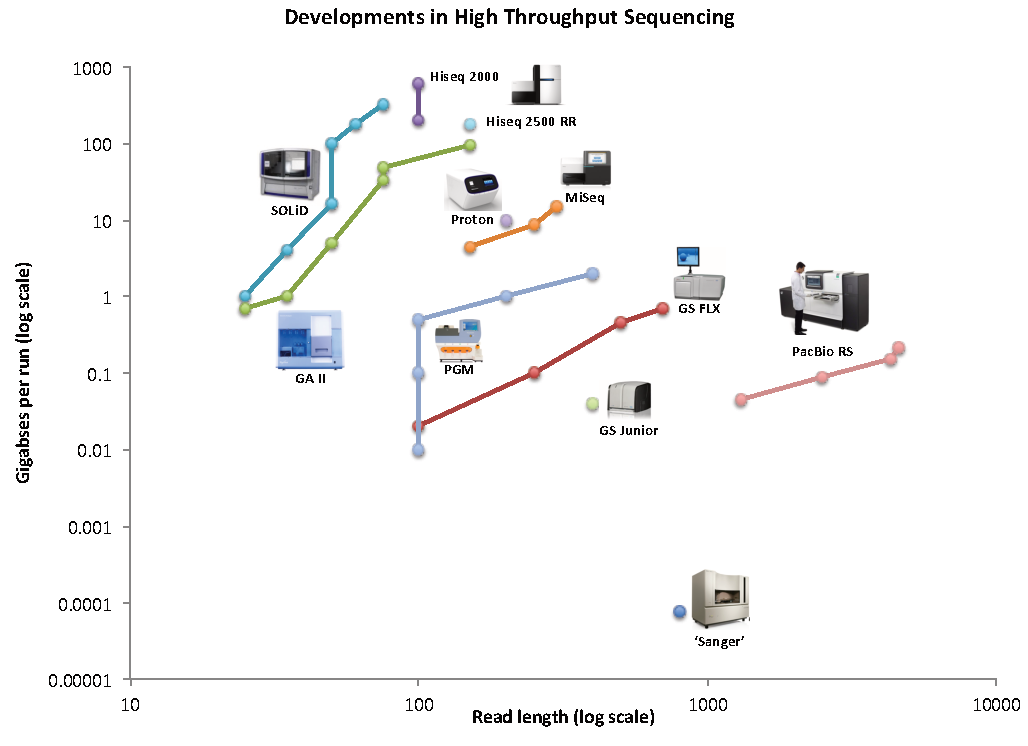
\includegraphics[scale=.5]{images/chapter3/figure3_1.pdf} % requires the graphicx package
   \caption[Current Sequencing Technologies]{Current sequencing technologies. On the x-axis is the current read length for each sequencing platform. The y-axis is the bases per run. Each point is a new iteration of that platforms sequencing read length and coverage. HiSeq has the most coverage with relatively short read lengths. Figure adapted from \citep{developmentinNGS:2012bs} }
   \label{fig:figure3_1}
\end{figure}
\begin{table}[t]
\centering
\resizebox{.99\linewidth}{!}{
\begin{tabular}{lllrrS[table-format=3.2]}
\toprule
\textbf{Platform}   & \textbf{Instrument}      & \textbf{Year} & \textbf{Reads per run} & \textbf{Read length (mode or average)} & \textbf{Bases per run (gigabases)} \\
\midrule
Sanger & 3730xl          & ND   & 96            & 800                           & 0.0000768                 \\
454        & GS20            & 2005 & 200,000        & 100                           & 0.02                      \\
454        & GS FLX          & 2007 & 400,000        & 250                           & 0.1                       \\
454        & GS FLX Titanium & 2009 & 1,000,000       & 500                           & 0.45                      \\
454        & GS FLX+         & 2011 & 1,000,000       & 700                           & 0.7                       \\
454        & GS Junior       & 2010 & 100,000        & 400                           & 0.04                      \\
IonTorrent & PGM 314 chip    & 2011 & 100,000        & 100                           & 0.01                      \\
IonTorrent & PGM 316 chip    & 2011 & 1,000,000       & 100                           & 0.1                       \\
IonTorrent & PGM 318 chip    & 2011 & 5,000,000       & 100                           & 0.5                       \\
IonTorrent & PGM 318 chip    & 2012 & 5,000,000       & 200                           & 1.0                         \\
IonTorrent & PGM 318 chip V2 & 2013 & 5,000,000       & 400                           & 2.0                         \\
IonTorrent & Proton PI       & 2012 & 50,000,000      & 200                           & 10.0                        \\
Illumina   & GA              & 2008 & 28,000,000      & 35                            & 1.0                         \\
Illumina   & GA II           & ND   & 100,000,000     & 50                            & 5.0                         \\
Illumina   & GAIIx           & 2009 & 440,000,000     & 75                            & 33.0                        \\
Illumina   & GAIIx           & 2011 & 640,000,000     & 75                            & 48.0                        \\
Illumina   & GAIIx           & 2012 & 640,000,000     & 150                           & 95.0                        \\
Illumina   & HiSeq 2000      & 2010 & 2,000,000,000    & 100                           & 200.0                       \\
Illumina   & HiSeq 2000      & 2011 & 3,000,000,000    & 100                           & 600.0                       \\
Illumina   & HiSeq 2500 RR   & 2012 & 600,000,000     & 150                           & 180.0                       \\
Illumina   & MiSeq           & 2011 & 30,000,000      & 150                           & 4.5                       \\
Illumina   & MiSeq           & 2012 & 30,000,000      & 250                           & 8.5                       \\
Illumina   & MiSeq           & 2013 & 30,000,000      & 300                           & 15.0                        \\
SOLiD      & 3               & ND   & 320,000,000     & 50                            & 16.0                        \\
SOLiD      & 4               & ND   & 2,000,000,000    & 50                            & 100.0                       \\
SOLiD      & 5500xl          & 2011 & 3,000,000,000    & 60                            & 180.0                       \\
SOLiD      & 5500xl W        & 2013 & 3,000,000,000    & 75                            & 320.0                       \\
PacBio     & RS C1           & 2011 & 36,000         & 1,300                          & 0.045                     \\
PacBio     & RS C2           & 2012 & 36,000         & 2,500                          & 0.090                     \\
PacBio     & RS C2 XL        & 2012 & 36,000         & 4,300                          & 0.155                     \\
PacBio     & RS II C2 XL     & 2013 & 47,000         & 4,600                          & 0.216                    \\
\bottomrule
\end{tabular}}
\caption[Current HTS Sequencing Platforms]{Figure adapted from \citep{developmentinNGS:2012bs}}
\label{tab:table3_1}
\end{table}

\subsection{Long Long HCDR3s are Established at Original Recombination}
Using first generation HTS sequencing technology, we first observed long HCDR3 sequences in the healthy HIV-naïve repertoire25. Although, long HCDR3s were known to exist26-28,they are mostly primarily found in chronically HIV-infected subjects9,29-31. This lead to a multiple hypothesis model about the origin of long HCDR3s in chronically infected patients (figure \ref{fig:figure3_2}). Given that long HCDR3 antibodies against HIV are highly mutated relative to other antibodies, it could be hypothesized that insertions and deletions (indels) due to somatic mutations could be responsible for the ‘elongation’ of a long HCDR3. These antibodies could be elicited by a chronic infection or heterogeneous prime-boost vaccine strategy, both of which will exhibit selective pressure for antibody maturation from germline sequence (figure \ref{fig:figure3_2}). This long HCDR3 origin model was known as the ‘mutation’ model.The alternate hypothesis was that long HCDR3s were established in the bone marrow at the time of original recombination and were found in the circulating repertoire at presumably, low frequency, or were selected against due to known issues associated with autoimmunity32-35. This is known as the ‘original recombination’ model.

These two models for the origin of long HCDR3s were the original focus for this project and are detailed in specific aims of Bryan Briney’s thesis and were tested by comparing immunoglobulin sequence repertoires for long HCDR3s to those of canonical length HCDR3s36. We can test these models based on two main assumptions about antibody maturation process. One, all antibodies are generated in the bone marrow from the germline repertoire and affinity mature in the lymph tissue37,38. Thus, an antibody that is recently recombined in the bone marrow would have fewer mutations than antibodies that have gone through multiple rounds of affinity maturation.  Figure \ref{fig:figure3_4}A top panel shows an analysis of peripheral B cell mean number of mutations as a function of HCDR3 length. Longer HCDR3s tend to have lower levels of somatic mutations. Figure \ref{fig:figure3_3}B top panel specifically shows the correlation for IgM and IgG class types that have undergone positive and negative selection.

The second assumption is that the affinity maturation process is associated with insertion and deletion events that are likely to be caused by somatic hypermutation associated proteins39-41. Figure \ref{fig:figure3_4}A and \ref{fig:figure3_4}B lower panels show a negative correlation to insertion-deletion associated (indel) percentage suggesting further evidence towards the ‘original recombination’ model.Finally, a statistically significant change in long HCDR3 percentage between naïve B-cells and class switched IgM and IgG B-cells indicates that these antibody sequences are present at original recombination and are selected against during maturation.

Although the original goal for the work done by Bryan Briney was to determine the genetic origin of HCDR3s, it confirmed a population, albeit a very small one, of very-long HCDR3 sequences that are the same length as many of the exceptional broadly neutralizing antibodies against HIV-1. This fortuitous conclusion, along with rapidly advancing throughput of HTS technology lead to the experimental rationale.

\begin{figure}[pb]
   \centering
   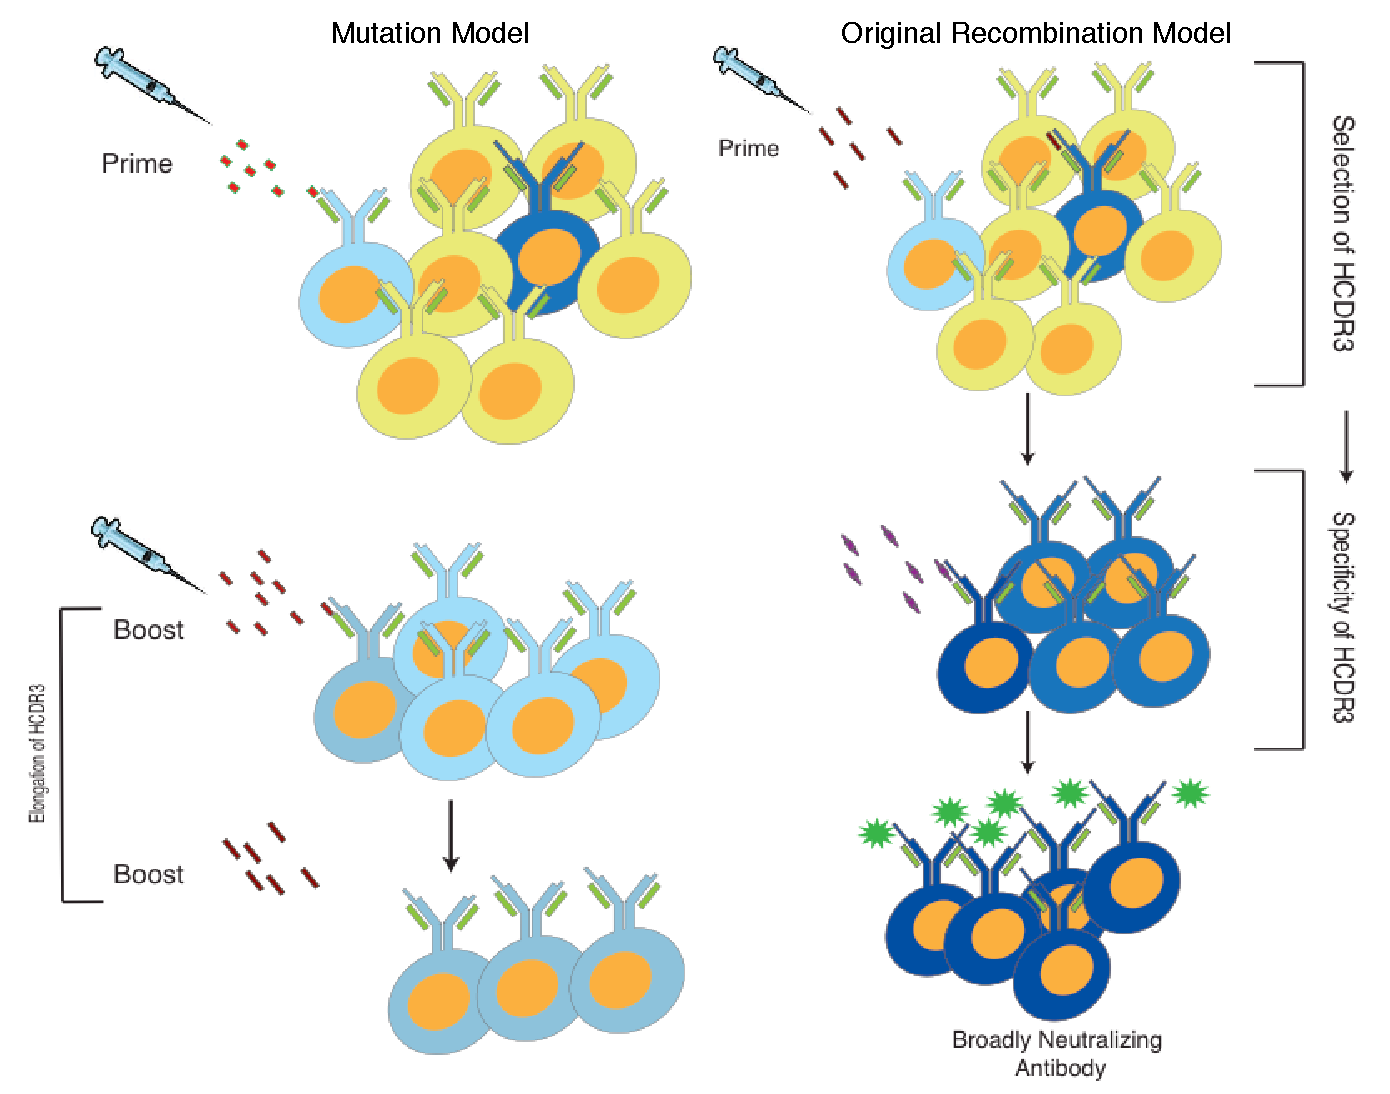
\includegraphics[width=.99\textwidth]{images/chapter3/figure3_2.pdf} % requires the graphicx package
   \caption[Origins of Long HCDR3 Models]{Origins of long HCDR3 models. Two models are proposed to explain the origin of HCDR3s. In the mutation model (left), B-cells (yellow) with canonical length HCDR3s are `elongated' through selective pressure on B-cells (blue) by chronic infection or repeated rounds of vaccine boosts to trigger affinity maturation to an evolving antigen. This repeated round of exposure creates insertions into the long HCDR3. The original recombination model (left) assumes the long HCDR3 is in low frequency in the naive population (yellow). Antigens from a vaccine or chronic infection select the infrequent B cell and expand its clonal population and refine affinity.}
   \label{fig:figure3_2}
\end{figure}

\begin{figure}[t]
   \centering
   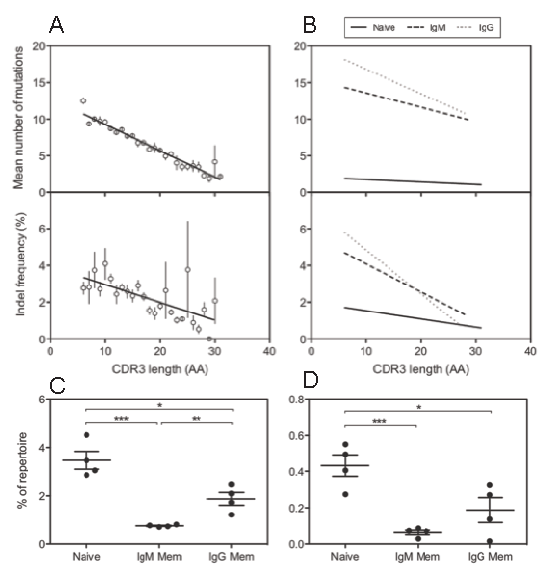
\includegraphics{images/chapter3/figure3_4.pdf} % requires the graphicx package
   \caption[Maturation Sequence Markers and HCDR3 Length]{Maturation Sequence Markers and HCDR3 Length. Insertion and deletion (indel) frequency and mutation frequency is associated as marker for affinity maturation and shows a negative correlation with HCDR3 length (A). The correlation becomes more pronounced in peripheral classed switched B cells IgM and IgG (B). The percentage of the repertoire with long HCDR3s (>24 amino acids, C) and very long HCDR3s (>28 amino acids, D) shows a statistically significant change from naïve B cells to class switched B cells (*** - p < 0.001, * - p < 0.1).}
   \label{fig:figure3_4}
\end{figure}

\subsection{Rationale and Experimental Design}
Our conclusions from examining the HIV naïve repertoire made me question approaches to HIV vaccine design. Traditional reverse vaccinology assumes that we can make a canonical antibody into a broadly neutralizing antibody by a series of prime-boost steps to achieve an optimal level of mutations to produce a protective response to HIV challenge. Indeed, many great strides have been made in the field42. However, the other unique trait about broadly neutralizing antibodies to HIV is many of them possess very long HCDR3s, were almost all of the contact and therefore mechanism of neutralization, stem from the long HCDR31,18,23,43.

With knowledge of the presence of long HCDR3s in HIV naïve donors, and that they are established at the time or recombination, we hypothesized that it was possible for these long HCDR3 sequences to converge on the structural space of some of the long HCDR3 driven broadly neutralizing antibodies. We choose the complex PG9 and a scaffolded epitope V1/V2 to be our template1. The goal was to see if we could mimic the 30-length HCDR3 in PG9 to neutralize HIV (PG9 mimicry). We chose PG9 with the following rationale.

\begin{enumerate}
    \item  The co-crystal structure had recently been elucidated(figure \ref{fig:figure3_3})1.
	\item  The long HCDR3 accounts for neutralization and functionality with few contact residues in other regions of the antibody17,18.
	\item  Germline reversions of the framework still retains neutralization ability12.
	\item  The RV144 trial, the first trial to show substantial vaccine efficacy correlated with an increase in V1/V2 binding antibodies, the binding region of PG944.
	\item  Interactions with the V1/V2 are structure dependent and sequence independent, i.e. backbone-backbone hydrogen bonding across beta-sheets1.
	\item  There is a 9 mutation difference between PG9 and it's sister antibody PG16 at the HCDR3 paratope showing a structural as well as functional convergence irrespective of sequence similarity9,17,18.
\end{enumerate}

The work of Bryan Briney with first generation high-throughput sequencing yielded a low frequency of sequences to test with a length of 30 (0.4\%). Building on this observation, figure \ref{fig:figure3_5} proposes an experimental plan that could test a large number of sequences for PG9 mimicry. In order to make the proposal feasible, we would have to upscale the amount of donors sequenced and the amount of B cell coverage in a new round of next-generation high-throughput sequencing.  We also knew that the coverage necessary was going to produce 500 million to 1 billion sequences, far more data than could be supported on our current architecture.

We planned to implement custom databases and search algorithms to recombine the sequences into a functional antibodyoyme. For prediction of PG9 mimicry, we also needed to develop a structural prediction scheme based on the package Rosetta that would rapidly be able to predict whether a sequence could tolerate the PG9 configuration. We also planned for a tractable amount of recombinant antibodies to be made in the laboratory to test for experimental validation using binding and neutralization analysis.

\begin{figure}
   \centering
   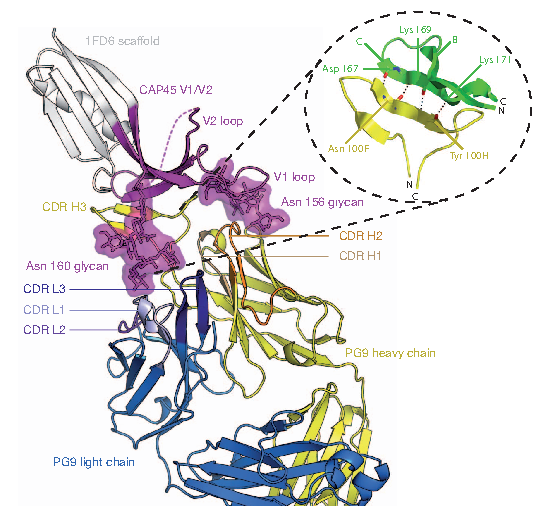
\includegraphics[scale=.8]{images/chapter3/figure3_3.pdf} % requires the graphicx package
   \caption[PG9 Complexed with V1/V2 Scaffold]{PG9 complexed with V1/V2 scaffold. The crystal structure adapted from \citep{McLellan:2011dg}. Beta-sheet interactions at the interface are highlted.}
   \label{fig:figure3_3}
\end{figure}

\begin{figure}
   \centering
   \includegraphics[width=.9\linewidth]{images/chapter3/figure3_5.pdf} % requires the graphicx package
   \caption[Overview of Methodology ]{The methodology can be split into four subsections that are a combination of computational (dashed-line) and experimental work (solid-line). HIV naïve blood is collected from 64 adult donors and the HCDR3 is sequenced on the HiSeq Illumina platform (A). The raw sequences are reconstructed and analyzed against germline databases using custom software. The sequences are parsed and stored in optimized databases to handle the large quantity of antibody sequences (B). HCDR3 sequences are chosen by length and tested for PG9 mimicry using the Rosetta software suite. Iterative rounds of minimization, docking, and design, followed by rigorous statistical analysis allows for a robust prediction of potential candidates from the HIV-naïve repertoire that may neutralize HIV (C). A tractable number of sequences are synthesized and tested experimentally through biophysical characterization and neutralization studies against HIV – 1 (D).}
   \label{fig:figure3_5}
\end{figure}

\section{Ultra High-Throughput Sequencing of HCDR3s}
As explained in the rationale, it was necessary to obtain many more sequences than were available using the coverage of 454-pyrosequencing. We decided to use the HiSeq platform, as the throughput at the time was 109 reads of 150 base pairs (bp). Although, the sequencing read of 150 bp was not long enough to cover the entire antibody variable gene, it would provide coverage of the HCDR3 portion of a recombined gene, sufficient for our experimental goals. We estimated that 0.4\% of the sequences would be greater than 28-length at 3 standard deviations from the mean HCDR3 length. This in theory would afford 400,000 recombined very-long HCDR3 reads.

Using the scheme found in figure \ref{fig:figure3_6}, we indexed 64 different healthy donors with based on a primer design by Bryan Briney and Jessica Finn. First, we obtained 64 HIV-naïve donors through the American Red Cross. No further information was obtained about each donor except for Hepatitis and HIV negative results. The mRNA was purified from the peripheral blood mononuclear cells (PBMC), and subjected to two rounds of PCR. The HiSeq run was done in the VANderibilt Technologies for Advanced GEnomics (VANTAGE). The raw data was reconstructed with paired-end algorithms and run through PyIg (Appendix). This program called on V, D, and J gene segments for the HCDR3 region and stored them to a database custom built for large amounts of information. The statistics for the HiSeq run are found in Table \ref{tab:table3_2}.  The full methodology can be found in the methods appendix section.

Next, we queried our database to get a distribution a frequency of HCDR3 lengths. Without removing any redundancies of amino acid sequences, we binned each length and got a distribution, referred to as all sequences (figure \ref{fig:figure3_7}A). We then removed all redundancies within each donor and plotted them as a function of length, referred to as donor unique (figure \ref{fig:figure3_7}A, B). Finally, we made a distribution that pooled all the sequences together and removed all HCDR3 redundancies, referred to as total unique (figure \ref{fig:figure3_7}A-C). The redundancies found in all donors combined subtracted by all unique sequences are by definition shared in at least one or more donor. For example, for length of HCDR3 equal to 1, we have 174 occurrences when we add up donor unique. That is, for donor 1 we have x amount of unique sequences among that donor added to x amount of sequences for donor 2 and etc. However, when we pool all the sequences of length 1 first, and then remove redundancies, we arrive at 17 unique sequences. That means there are 137 shared amino acid sequences found in one or more donors. An easier way to view it, is to plot the percentage of sequences at a given length that are shared among one or more donor (figure \ref{fig:figure3_7}D). This can actually be done with database queries that are detailed in the appendix.

The mean length of HCDR3 sequences in our dataset was 16.40 \pm 4.03. This was in previous agreement with our work using a much smaller dataset25. Although there is no standard definition of a `'long HCDR3' we arbitrarily chose the cutoff to be two and three standard deviations from the mean for long and very long HCDR3s respectively (24AA, 28AA, Figure \ref{fig:figure3_7}C).Our recombination software (PyIg) can also assign V, D, and J gene families using the BLAST algorithm45. We observed similar trends in D and J gene family usage as a function of length. DH3 and JH6 family increased as length of HCDR3 increased (figure \ref{fig:figure3_7}F, G). This makes intuitive sense these are the longest gene segments in their respective segment. For V-gene families, we did not observe a different in germline gene usage as a function of length (figure \ref{fig:figure3_7}E). This trend was also reported with our previous work in which we sequenced the entire antibody segment, however, we can’t be absolutely confident in our assignments of V-gene considering we only have on average a 20 bp overlap. We can also narrow down individual genes for the D-gene segment and observed an increase in DH2-2, DH2-15, DH3-3, DH3-10 and DH3-22 as HCDR3 length increased (figure 3.7H).  With a full dataset, we were ready to begin predictions for long HCDR3s that can mimic PG9 using the Rosetta software suite.

\begin{figure}
   \centering
   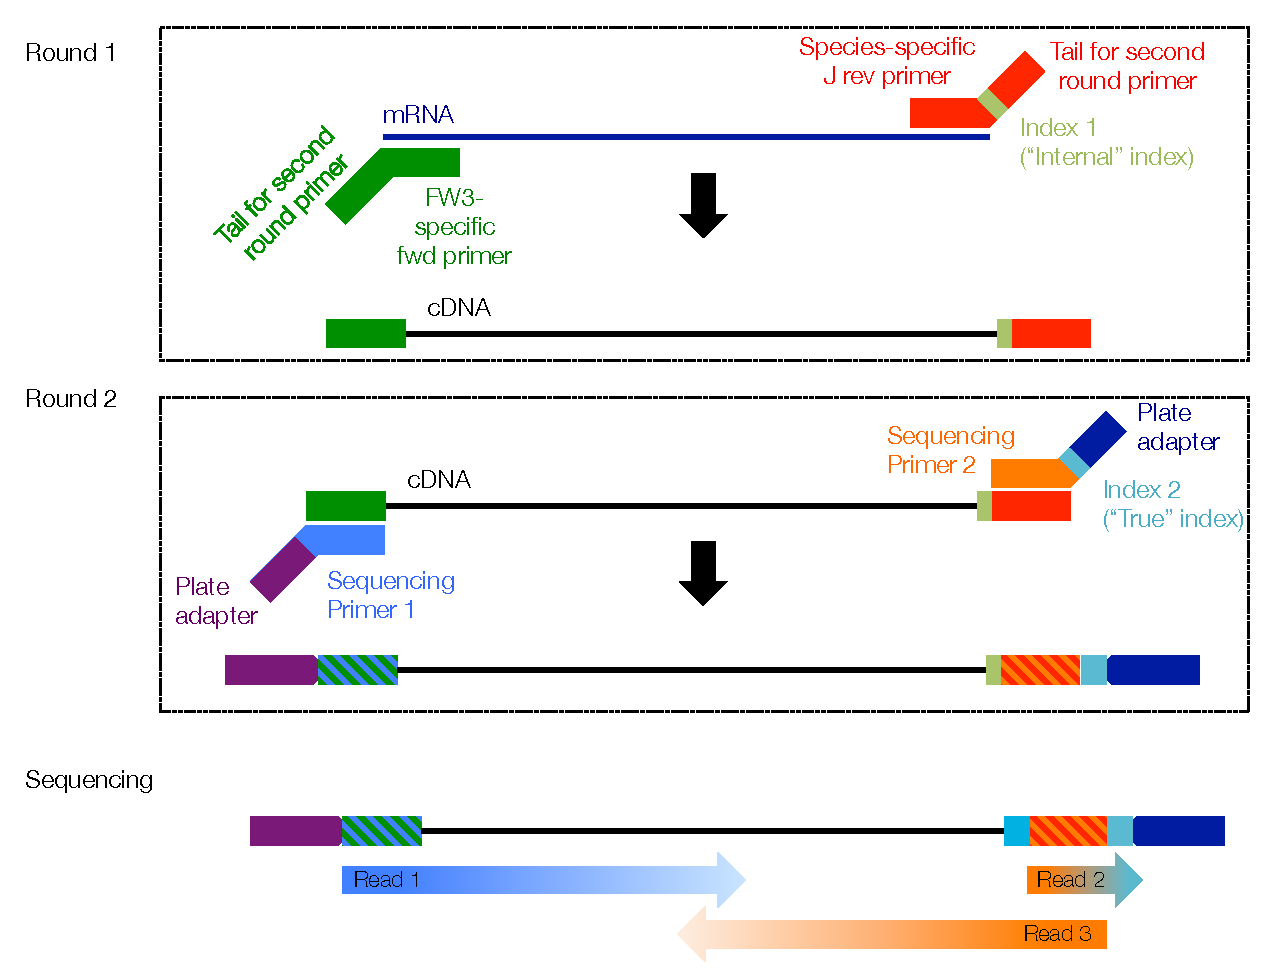
\includegraphics[width=.9\linewidth]{images/chapter3/figure3_6.pdf} % requires the graphicx package
   \caption[Overview of HiSeq Scheme]{RT-PCR in round 1 allows addition of an internal index to categorize donors. The cDNA is then subjected to a nested round 2 PCR where the necessary HiSeq plate adaptors and sequencing regions are added that are used by Illumina. The sequencing makes two pair-end reads that are later reconstructed.}
   \label{fig:figure3_6}
\end{figure}

\begin{figure}
   \centering
   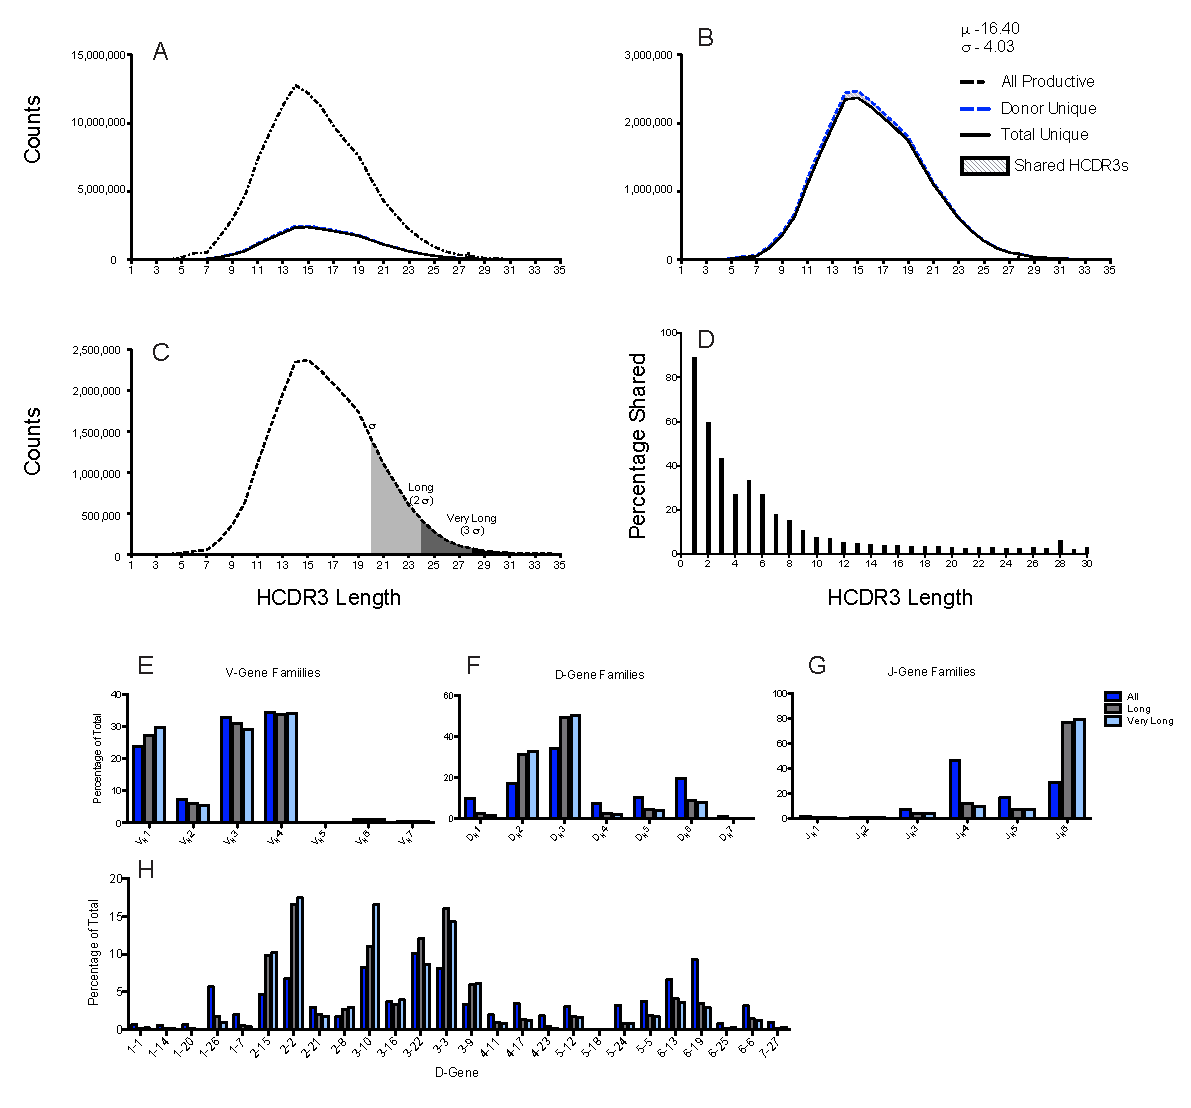
\includegraphics[width=.9\linewidth]{images/chapter3/figure3_7.pdf} % requires the graphicx package
   \caption[Distribution and VDJ gene Usage]{Length distribution for all productive sequences (black dashed line), unique among within each donor (blue dashed) and unique among every donor (black solid) (A). Zoomed in distribution of total unique and donor unique to see overlap. Sequences that are unique between donors are shaded in grey lines (B). Total unique with standard deviations shown at 20, 24, and 28 (C). Percentage of shared sequence as a function of HCDR3 length. Shared sequence is defined as being found in two or more donors (D). V-gene families, D-Gene families and J-Gene family frequencies for all sequences, long, and very long HCDR3 sequences (E, F, G respectively). D-gene families can further be divided into individual gene frequencies for all, long, and very long HCDR3 sequences (H).}
   \label{fig:figure3_7}
\end{figure}
\begin{SCtable}
\centering
\begin{tabular}{rr}
\toprule
\textbf{Metric}        & \textbf{Counts} \\
\midrule
Raw Reads              & 514,312,664     \\
Joined Reads           & 460,931,435     \\
Unique Reads           & 167,667,706     \\
Recombinant Reads      & 159,609,585     \\
Productive CDR3s       & 118,440,255     \\
Unique CDR3s by AA     & 23,357,390      \\
30 Length CDR3s        & 74,457          \\
Unique 30 Length CDR3s & 24,917         \\
\bottomrule
\end{tabular}
\caption[HiSeq 64-Donor Statistics]{Sequencing results from the HiSeq of 64 donors. Raw reads indicate the amount of reads that passed VANTAGE quality metrics. Joined reads are reads that found a paired end partner and could be joined together. Unique reads removed duplicates. Productive HCDR3s are those reads that do not contain a stop codon. Unique CDR3s are those HCDR3s that are not duplicated by amino acid sequence. 30 length HCDR3s are those sequences that are 30 amino acids long by IMGT numbering. Unique HCDR3 sequences are those sequences that are not duplicated in any donor by amino acids.}
\label{tab:table3_2}
\end{SCtable}


\section{Addition of Non-Canonical Amino Acids in Rosetta}
The Rosetta software suite was initially developed for ab initio folding of small globular proteins using fragment-based search methods and knowledge-based potentials to score models46. Because of this, the code for Rosetta made protein amino acid residues the smallest object. All proteins would be made up of residue objects, and all ‘building blocks’ would be made up of parameters that describe your residue object. This made sense at the time of Rosetta’s inception given its primary purpose, but as it’s scoring function was being developed for a wide variety of molecular modeling tasks, the residue based code became difficult to implement for non-residue type molecules, i.e. drug-type ligands, glycans, and post-translational modifications.

The PG9 complex relied on complex and high-mannose type glycans that were bound to asparagine residues at position N160 and N156 (HXBc2 numbering) 19. Removal of these residues abrogated binding to HIV envelope47. Thus, it was necessary to include both of these glycans in our predictions. It was also necessary to encode these glycans as non-canonical amino acid residues rather than post-translational modification due to the residue object requirement of Rosetta score function. We based the protocol of adding the two non-canonical amino acids after the work of Renfrew and colleagues who developed a generalized protocol for implementing non-canonical amino acids into Rosetta48. The protocol used a series of steps that we loosely followed that involved extraction of the residue, minimization of the residue using quantum mechanics simulations, and description of the new amino-acid types as a series of parameters that Rosetta can recognize. We first had to benchmark the non-canonical amino acid types before we could use them in the protocol. To do this we ran minimization and design against the glycan and determined if our best scoring models were the closest to the native structure found in the PDB. The best scoring model according total energy was aligned with the native structure, we saw minimal deviation from the native structure indicating that for good scoring models, the glycan conformation is preserved (figure \ref{fig:figure3_8}A). A general trend between the glycan score and the total score as a function of the glycan RMSD (the deviation from the native conformation) was observed indicating that the glycan tolerating the Rosetta scoring function (figure \ref{fig:figure3_8}B). We also observed that PG9 HCDR3 amino acids were ideal for antibody-antigen complex during redesign of the PG9-antigen (figure \ref{fig:figure3_8}C). With these data, we could proceed with the threading protocol with incorporated glycans.

\begin{figure}
   \centering
   \includegraphics[width=.9\linewidth]{images/chapter3/figure3_8.pdf} % requires the graphicx package
   \caption[Glycan Addition and Benchmarking Template]{Glycan addition and benchmarking template. Energetically minimized loop of the PG9 HCDR3 overlaid on the native PG9-antigen complex (PDB-3U4E).14 Native PG9-antigen is shown in darker colors while the redesigned, energetically minimized and re-docked structures are shown in lighter colors. Light is chain is shown in blue, heavy chain grey, and antigen in magenta. The two glycans are shown in stick representation. The native glycan positions are shown in transparent stick conformation (A). The score of the glycan and the score of the model are shown as a function of the glycan RMSD. On the y-axis are Rosetta scores, and on the x-axis is the glycan RMSD from native structure found in the PDB. The top panel is the total energy of the complex compared with the glycan RMSD while the bottom compares the glycan score to the glycan RMSD. A general trend is shown between the glycan deviation from native conformation and an increase in score (B). Sequence logo of redesigned HCDR3 loop of PG9 with glycans present. The x-axis shows PG9 native sequence (C).}
   \label{fig:figure3_8}
\end{figure}


\section{High-Throughput Threading of HCDR3 Sequences}
We took 4000 random HCDR3 sequences from an available dataset of 26,417 (table \ref{tab:table3_2}). These sequences were “threaded” over the PG9 HCDR3 backbone and energetically minimized. We did not include the antigen in this first set of modeling experiments as it our first goals were to establish a high-throughput prediction model of PG9-like antibodies and not necessarily anti-HIV gp120 neutralizing antibodies. This was for an experimental contingency in case our modeling experiments predicted that none of our sequences could bind gp120 antigen.

The threading protocol removes amino acid sequence identity of the HCDR3 loop and replaces, or “threads”, one of the 4000 random HCDR3 sequences from our dataset. After they amino acid identity has been replaced, the PG9 antibody is energetically minimized and scored with the Rosetta scoring function (detailed in the document introduction).

Considering each model took approximately 1.2 CPU hours to complete at the computing cluster (https://vanderbilt.accre.com) at the time of writing, all 26,417 models would have taken 31,700 CPU hours to complete. Considering Rosetta takes approximately 1000-10000 models to determine energy landscape50-54, we were approaching CPU times from 3.17 x 10$^{7}$–3.17 x 10$^{8}$ hours. I could utilize approximately 600 processors running in parallel, cutting down CPU times to 52,834 hours or ~6 years. Obviously these numbers were unrealistic at the time of writing, so we decided to optimize heuristics methods that could be accomplished with a far fewer number of models. We chose 4000 random sequences with 50 models as a strict cutoff to maximize data output within the capabilities of our computational resources.

To evaluate the threading protocol, we scored our models using the Rosetta scoring function and plotted it against the deviation from PG9s native structure (figure \ref{fig:figure3_9}A). As a control, PG9 and PG16 are also put into the threading protocol to evaluate the scoring functions ability to make distinctions between poor scoring and favorable scoring models. Considering we know that PG9 and PG16 sequences form to PG9s backbone conformation, we expect a very low deviation from PG9s crystal-structure conformation. We also expect Rosetta’s scoring function to score these sequences as favorable relative to many of the random HCDR3s that were evaluated in the protocol. Indeed, we observed that PG9 and PG16 consistently rank as the most favorable in terms of score and conformation and confirm the accuracy precision of our threading protocol (figure \ref{fig:figure3_9}A).

In contrast, the random 4000 HIV-naïve HCDR3 sequences tend to group into three separate categories. Those sequences which maintain the HCDR3 structure of PG9, but score poorly (figure \ref{fig:figure3_9}B), sequences which score well but collapse or deviate away from PG9 native conformation (figure 3.9D), and finally sequences which score well and retain PG9 conformation (figure \ref{fig:figure3_9}C). These three groups give a diverse sequence-energy landscape to be carried on into our heuristics in order to evaluate the remaining ~22,000 HCDR3 sequences.

\begin{figure}
   \centering
   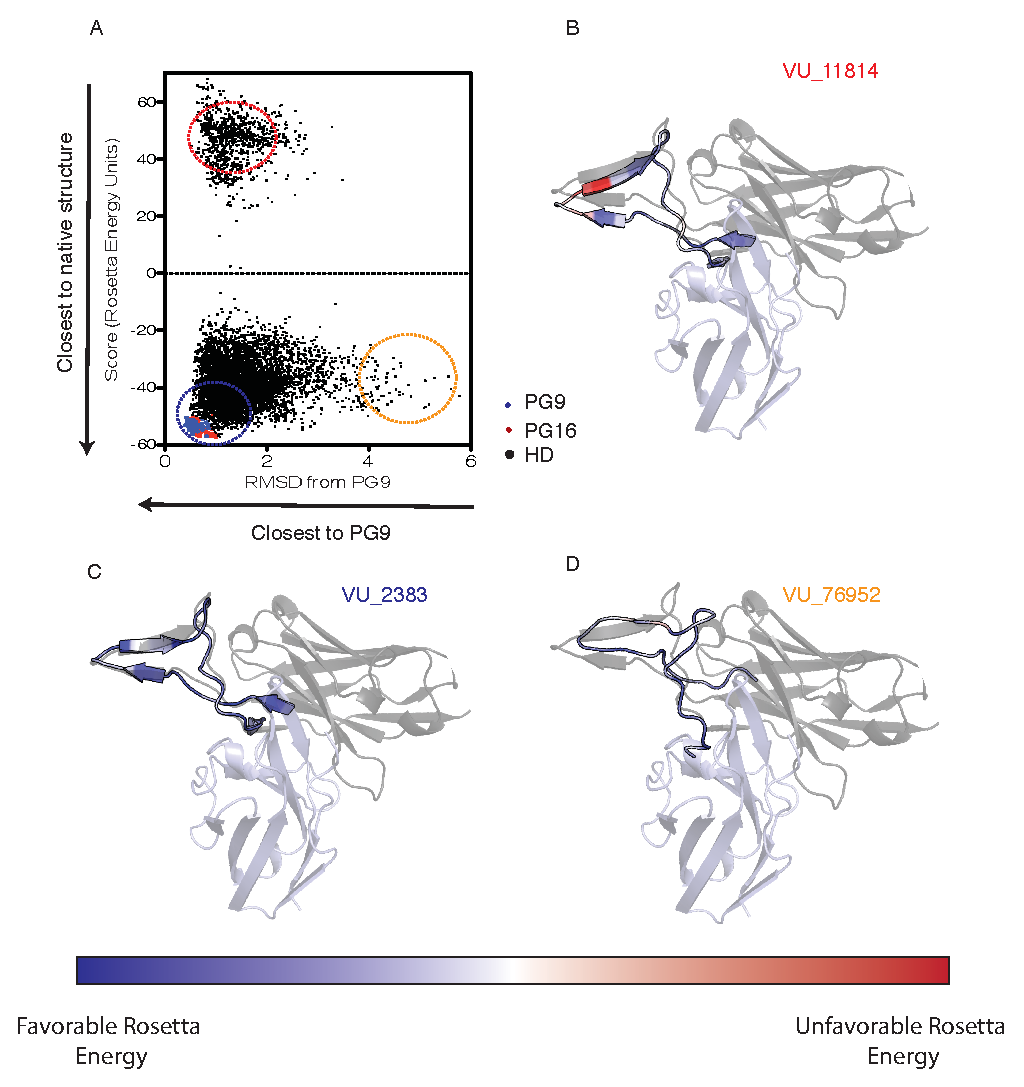
\includegraphics[width=.9\linewidth]{images/chapter3/figure3_9.pdf} % requires the graphicx package
   \caption[Threading PG9 Produces Three Structural Outcomes ]{The threading protocol for PG9 is evaluated for structural mimicry and against the Rosetta scoring function. The models scores are evaluated and plotted against the root mean squared deviation (RMSD) from the native PG9 HCDR3 structure. Lower scoring models are closer to native structure (y-axis) while models closer to PG9 HCDR3 structure have a lower RMSD (x-axis). Repeated measures of PG9 and PG16 are grouped close to native structure and close to PG9 structure (blue and red points) while HIV naïve antibody sequences are shown are labeled HD (black points) (A). For figured B-D, HCDR3 structures are aligned to native PG9 (shown in transparency). The HCDR3s are colored by their Rosetta score with blue being a favorable scoring residue and red being an unfavorable score. There are three different outcomes observed for the threading experiment. Sequences which can retain PG9 structure but produce an unfavorable score (B, dashed red circle in figure A), sequences which produce a favorable score but collapse away from PG9 native structure (D, dashed orange circle in figure A), and sequences which score favorably and adopt PG9 conformation (C, blue dashed circle in figure A).}
   \label{fig:figure3_9}
\end{figure}


\section{Heuristics to Rapidly Score HCDR3 Sequences}
Using the 4000 HIV-naïve HCDR3 sequences, we randomly choose half of the sequences to be in the benchmark set or the training set. For the training set, 2000 sequences were evaluated with the Rosetta scoring function and for each position 96-125 (PDB numbering), we filled a position structure specific scoring matrix (P3SM). For each position, and each amino acid identity, we gave an initial score of 0.0 to baseline yielding a 20 x 30 matrix, and averaged each amino acid identity score at each position (figure \ref{fig:figure3_10}A,B). The matrix can be visualized as a heat map with favorable scores in blue and unfavorable scores in red (figure \ref{fig:figure3_10}B).

The P3SM now becomes our heuristic to rapidly score other sequences that were not run through the computationally expensive threading protocol. We can validate our heuristic by evaluating how well the P3SM does at predicting Rosetta energies by applying it to the other 2000 sequences in the benchmark set. The P3SM may not give absolute Rosetta energies but should provide a relative ranking compared to other HCDR3 sequences. We observe a 0.863 r2-value for a correlation between actual Rosetta energies and P3SM predicted energies. For the top 10\% energies evaluated by the Rosetta energy function, our correlation falls to 0.300 (figure \ref{fig:figure3_10}C).

To determine the relative noise of the P3SM, we ranked the scores and determined the position of PG9. It was found in 104th position out of all 26,417 sequences (0.3\%). The difference in the PG9 P3SM score and the top scoring sequence was 3.82 Rosetta energy units. Thus, the final noise tolerance of our matrix was -34.84 ± 3.82 (-31.02 to 38.66) which encompassed approximately 1000 sequences (figure \ref{fig:figure3_10}D). We then define our P3SM heuristic to be able to accurately pick out the top 1000 out of 26,417 sequences (3.79\%).

\begin{figure}
   \centering
   \includegraphics[width=.9\linewidth]{images/chapter3/figure3_10.pdf} % requires the graphicx package
   \caption[Heuristics Predict HCDR3 Sequences that Mimic PG9 Structure]{Heuristics predict HCDR3 Ssquences that mimic PG9 structure. 2000 random models are evaluated at each amino acid position. A cartoon representation of the HCDR3 loop is shown with each position colored with a blue-red gradient according to favorable to unfavorable amino acid identities, respectively (A). Each position is initially assigned a score of 0.0 and enumerated through averaging each amino acid identity with the score to fill a position structure specific scoring matrix (P3SM) from 2000 HCDR3 sequences. The matrix can then be used to rapidly score the other 2000 models that were not used to fill the matrix to predict a Rosetta score (B). A simple linear regression can be applied to the actual Rosetta energy score of a sequence and its predicted score to give a coefficient of determination (r$^{2}$) of 0.863. When only the top 10\% by actual Rosetta score are considered the coefficient of determination drops to 0.330 (C). Using the P3SM, PG9 scored 104th. Calculating the difference in score between the top scoring sequence and PG9 left a noise tolerance of 3.82 Rosetta energy units (REU). Calculating \pm 3.82 REU of PG9 leaves 1000 HCDR3 sequences that fall within the noise tolerance range of the P3SM (D).}
   \label{fig:figure3_10}
\end{figure}


\section{Docking and Minimization of HCDR3 Variants}
With 1000 candidate sequences from the original sequence pool of 26,417, we ran the threading protocol again in the presence of the antigen and complex glycans that were added from earlier sections (see addition of non-canonical amino acids). The threading protocol was modified slightly to include all atom constraints, and an additional docking step and 100 models generated for each sequence (100,000 models). The full protocol is detailed in the methods section of the appendix.
In addition to PG9 deviations and total scores, we also evaluated binding energies, which are the change in free energy (ΔΔG). We define the ΔΔG as follows.

%$\Delta\DeltaG_{Complex} = \deltaG_{Bound} - \deltaG_{Unbound}$

Where,

%$\DeltaG_{Bound} = RosettaScore_{Complex}$ and  $\DeltaG_{Unbound} = RosettaScore_{Seperated}$

We decompose the binding energies, total energies, and deviations into several metrics to evaluate the models. Total energy, binding energy, and deviation (C$\alpha$ - RMSD) for just the HCDR3 portion of the model, the binding energy contribution by both of the glycans (N156 $\delta\delta$G and N160 ΔΔG, HxBC2 numbering), and the total binding energy for the entire model.

Initially each of these metrics can be evaluated individually to see where they rank or in pairs by plotting them against each other (figure \ref{fig:figure3_11}, left panel). Favorable sequences will be in near PG9 in the plot. We can also plot HCDR3 metrics as heat maps and score models qualitatively (figure \ref{fig:figure3_11}, right panel). Both of these methods are inefficient as each metric produces a different rank ordering of the HCDR3 sequences. Therefore, we sought to combine these six metrics into one encompassing score to easily compare where each sequence ranks in comparison to PG9.

To combine the metrics, we assigned a simple Z-score to each metric to find out where that model ranked. The Z-score can then be weighted and averaged for each scoring metric to produce a weighted Z-score that can be used to efficiently rank sequences with one score using the following equation:

$Weighted Z = $

Where w\textsubscript{i} is the weight of each Z-score statistic i, Z\textsubscript{i} is the z score for the statistic i, and N is the total number of statistics. The addition of the weights allowed optimization during ad hoc analysis to ensure PG9 and PG16 were the most favorable weighted Z-score. The final weights used in the protocol were: total ΔΔG – 3.0, HCDR3 ΔΔG - 1.0, HCDR3 total score – 1.0, N156 ΔΔG – 0.5, N160 ΔΔG – 0.5 and HCDR3 C$\alpha$-RMSD - 0.5. We chose the top 80 HCDR3 HIV naïve sequences to carry on to experimental steps, as this number was our upper limit to synthesize.

\begin{figure}
   \centering
   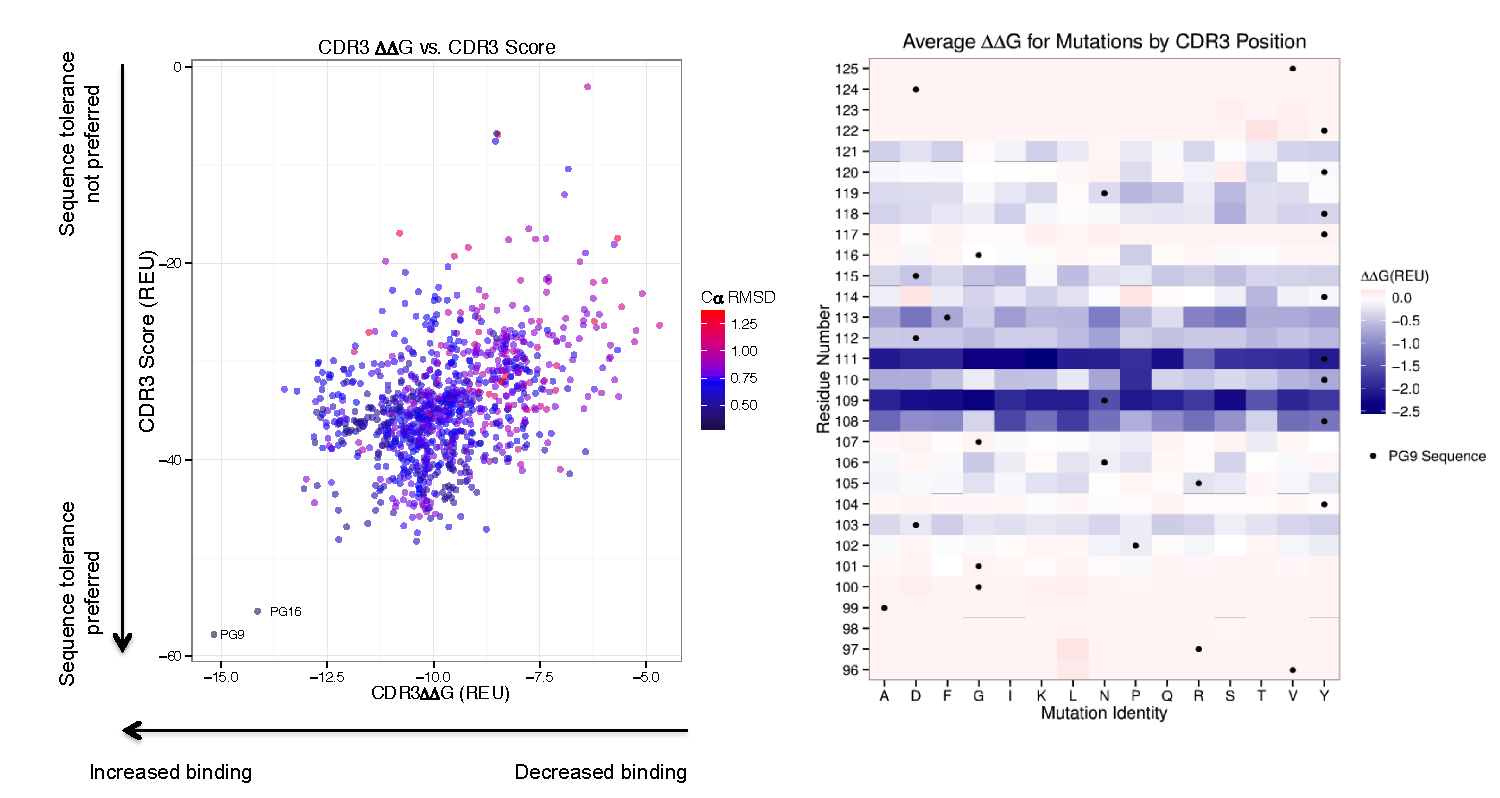
\includegraphics[width=.9\linewidth]{images/chapter3/figure3_11.pdf} % requires the graphicx package
   \caption[Scatter Plots and Heat Maps for P3SM Threading Analysis]{Scatter plots and heat maps for P3SM threading analysis. Each metric can be plotted on a separate axis and sequences which are found to score well are found in the lower left of the graph. For example, HCDR3 binding energy is plotted against HCDR3 score. PG9 and PG16 are found to have favorable binding energy and score (left panel). A heat map can also be generated for each metric for residues in the HCDR3. For example, contribution to binding energy for each amino acid identity can be plotted as a heat map. The red to blue scale is for neutral to favorable reactions (right panel)}
   \label{fig:figure3_11}
\end{figure}

\section{Clustering of HIV-Naïve Sequences}
Rather than synthesize all 80 HIV-naïve sequences that were predicted to be closest to PG9 mimics, we instead considered that several of the sequences were related siblings to each other. Indeed, upon clustering at a threshold 85\% amino acid similarity (4 mutations), the sequences clustered into nine different groups and five sequences formed independent groups (figure \ref{fig:figure3_12}).
We next aligned the nucleotide and amino acid sequences to find sequence similarities among each of our PG9 clustering groups. Surprisingly, only the beginning and end of the sequences corresponding to the base of the HCDR3 displayed a high degree of similarity (figure \ref{fig:figure3_12} A-B).

The similarity arises from the in-frame J\textsubscript{H}-6 gene for most long HCDR3 sequences with the exception of cluster I and IG2, which used J\textsubscript{H}-4 and had significant J-gene exonuclease activity, respectively (table \ref{tab:table3_3}). We also detected some nucleotide conservation for positions 27-36 corresponding to amino acid 9-12, which is a semi-conserved SSGY motif (figure \ref{fig:figure3_12} A-B). Rather than synthesize and express each of the 80 variants, we chose to synthesize one member from each cluster and one of the sequences that did not cluster. These sequences were selected based on their Rosetta weighted Z-score metric within each cluster (table 3.4).

\begin{figure}
   \centering
   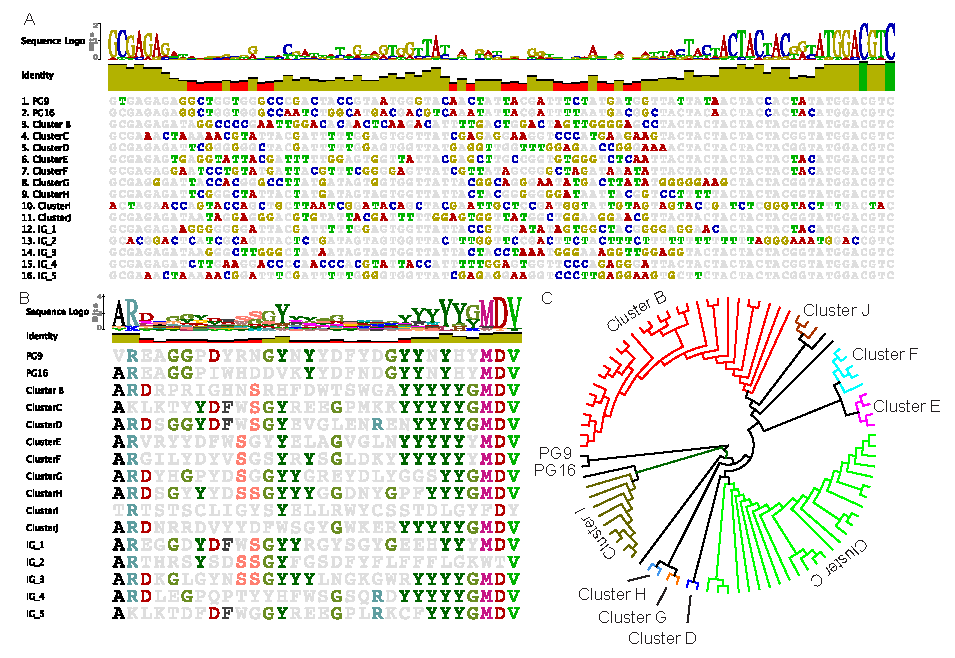
\includegraphics[width=.9\linewidth]{images/chapter3/figure3_12.pdf} % requires the graphicx package
   \caption[PG9-Mimicry Candidates Cluster Into Groups]{PG9-mimicry candidates cluster into groups. The consensus nucleotide sequence is aligned for each cluster B-J. There is little sequence similarity in the junctions except for the VH and JH gene. Sequence logo representations are shown above the sequence to detect conservation. Five independent group sequences are also shown (A). The same as (A) translated. Conserved elements are shown in the JH region due to conserved use of the JH6 gene family (B). The cladogram for each HCDR3 amino acid sequence shows how the top 80 sequences cluster into 9 groups with some groups having multiple sequences that differ by 1-4 amino acid mutations but are derived from the same lineage (C).}
   \label{fig:figure3_12}
\end{figure}
\begin{table}
\centering
\resizebox{.99\linewidth}{!}{
\begin{tabular}{lllllccccc}
\toprule
\textbf{Cluster} & \textbf{Members} & \textbf{V\textsubscript{H}} & \textbf{V\textsubscript{D}} & \textbf{V\textsubscript{J}} & \textbf{V-D Length} & \textbf{D-J Length} & \textbf{D 5'-Exo} & \textbf{D 3'-Exo} & \textbf{J-Exo} \\
\midrule
B                & 29               & V3-07*01    & D3-09*01    & J6*02       & 21                  & 15                  & 3                 & 10                & 2              \\
C                & 25               & V4-34*01    & D3-03*01    & J6*02       & 10                  & 24                  & 0                 & 6                 & 2              \\
D                & 2                & V1-46*01    & D3-03*01    & J6*02       & 9                   & 25                  & 4                 & 6                 & 3              \\
E                & 4                & V1-02*02    & D3-03*01    & J6*03       & 4                   & 23                  & 0                 & 4                 & 0              \\
F                & 5                & V4-34*01    & D3-16*02    & J6*03       & 9                   & 15                  & 4                 & 2                 & 0              \\
G                & 2                & V1-02*02    & D3-22*01    & J6*02       & 16                  & 16                  & 7                 & 3                 & 10             \\
H                & 2                & V4-04*02    & D3-22*01    & J6*02       & 6                   & 23                  & 1                 & 0                 & 8              \\
I                & 9                & V4-34*12    & D2-02*01    & J4*02       & 54                  & 9                   & 4                 & 12                & 2              \\
J                & 3                & V3-07*01    & D3-03*01    & J6*02       & 14                  & 14                  & 0                 & 6                 & 1              \\
IG1              & 1                & V3-07*01    & D3-03*01    & J6*03       & 8                   & 29                  & 2                 & 4                 & 9              \\
IG2              & 1                & V2-70*01    & D3-22*01    & J6*02       & 10                  & 48                  & 3                 & 7                 & 25             \\
IG3              & 1                & V1-02*02    & D3-22*01    & J6*02       & 11                  & 21                  & 6                 & 0                 & 5              \\
IG4              & 1                & V1-03*01    & D3-03*02    & J6*02       & 17                  & 9                   & 0                 & 8                 & 0              \\
IG5              & 1                & V4-34*01    & D3-03*01    & J6*02       & 12                  & 29                  & 2                 & 6                 & 7              \\
PG16             & 1                & V3-33*05    & D3-03*01    & J6*03       & 34                  & 9                   & 1                 & 18                & 2              \\
PG9              & 1                & V3-33*05    & D3-03*01    & J6*03       & 34                  & 0                   & 1                 & 2                 & 9      \\
\bottomrule
\end{tabular}}
\caption[Gene Usage Statistics of PG9-Mimicry Clusters]{Each of the nine clusters and independent sequences (IG1-5) and their representative V, D, and J genes are shown. V-D and D-J lengths are the nucleotide lengths of those junctions. D 5'-, D 3'-, and J-Exo were the amount of nucleotides excised in the junctions to make a productive recombination. Point mutations in the junction are not shown.}
\label{tab:table3_3}
\end{table}



\section{Design of Top PG9-Mimicry Candidates}
We realized that these wild-type sequences sometimes contained clashes or caused other steric strain of the HCDR3 loop that was reflected in the difference in normalized Z-scores (table \ref{tab:table3_4}) or as an energetic gap between the predicted energies of PG9 and the top 80 variants selected (figure \ref{fig:figure3_13}A). It was because of this we decided to run a dock-design protocol that would relieve clashes and strains for unfavorable amino acids. We also imposed a filter that gave bonuses for amino acids that were native to the starting sequence. It was in this way, we were able to attain predicted PG9 mimicry by lowering the energetic gap while retaining as many wild-type sequences as possible (figure \ref{fig:figure3_13})We chose a variant from each cluster whose sequence recovery (the percentage of designed sequences that were wild-type) and carefully analyzed each predicted mutation suggested by Rosetta. We ranked the mutations based on a fitness score. We defined the fitness core as the change in total score for the mutation from the wildtype added to the change in binding energy for the mutation compared to wildtype. If the fitness was found to be significant, the mutation was confirmed by visual inspection.

Briefly, I will explain the rationale for choosing the mutations for cluster B. Variant VU42252 was chosen as the representative candidate for design since it provided the best sequence recovery to the wild-type sequence as well as beneficial fitness (figure \ref{fig:figure3_14}A). Each mutation is plotted as a function of its fitness and grouped together by position (figure \ref{fig:figure3_14}B). If there is a large decrease in energy from the wild-type sequence, it corresponds to a beneficial fitness for a given mutation. Those mutations that had a favorable change in fitness with a magnitude of greater than 1.5 Rosetta energy units were manually inspected (figure \ref{fig:figure3_14}C,D). Two such mutations are shown at position 106 (figure \ref{fig:figure3_14}C) and position 120 (figure \ref{fig:figure3_14}D). For position 106, the wildtype serine is not preferred since it leaves a large exposed gap between the antigen face and the antibody interface. Upon mutation to an asparagine, the gap is filled in. Additionally the asparagine makes new hydrogen bond contacts with the antigen. This is predicted to benefit the binding energy and stabilization of the complex. Position 120 has a wild-type tyrosine that repels against the large steric bulk of the glycan. A mutated asparagine at this position allows an inter-HCDR3 hydrogen bonds to stabilize the loop while also making additional hydrogen bonds to the glycan.

For cluster B, we chose six different positions to be mutated alone or in combinations that produced five different candidate variants. This totals six different variants to try for cluster B, one wildtype sequence, and five mutational variants that range from 3-10 mutations. The remaining clusters were analyzed similarly and in total, 10 wildtype sequences were chosen for experimental characterization and 74 different sequences that were mutational variants of the representative cluster sequence.

\begin{table}[!h]
\centering
\begin{tabular}{lc}
\textbf{Cluster}   & \textbf{Weighted Z-Score} \\
\hline
Cluster B & -1.24            \\
Cluster C & 0.28             \\
Cluster D & 0.11             \\
Cluster E & 0.15             \\
Cluster F & -0.34            \\
Cluster F & -0.20            \\
Cluster G & 0.31             \\
Cluster H & 0.11             \\
Cluster I & -2.54            \\
Cluster J & 1.48             \\
PG9       & -4.80            \\
PG16      & -1.87            \\
IG 4      & -1.46
\end{tabular}
\caption[Weighted Scores of PG9-Mimic Clusters]{Weighted scores of PG9-mimic clusters. Each cluster with the top scoring sequence is shown with weighted Z-score.}
\label{tab:table3_4}
\end{table}
\begin{figure}
   \centering
   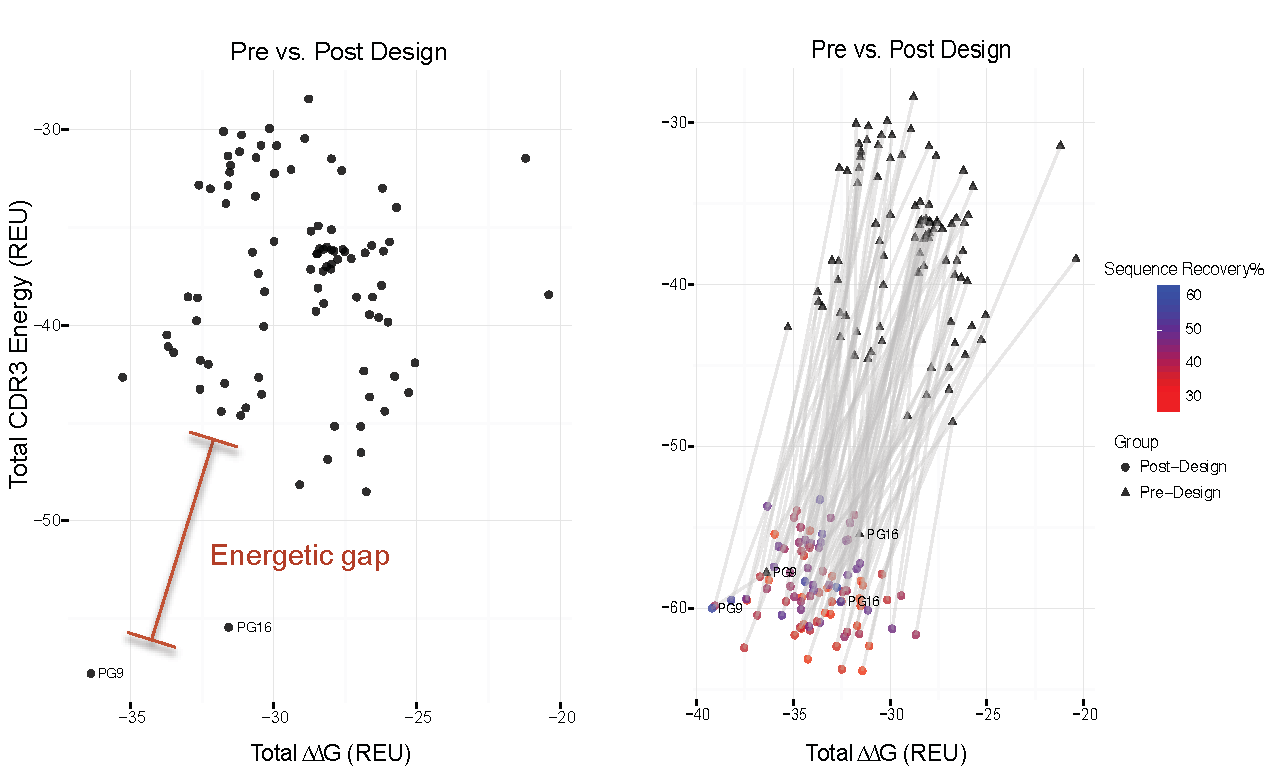
\includegraphics[width=.9\linewidth]{images/chapter3/figure3_13.pdf} % requires the graphicx package
   \caption[Energetic Barriers for Complete PG9-Mimicry]{Energetic barriers for complete PG9-mimicry. The total HCDR3 energy and binding energy are plotted for the top 80 sequences selected by normalized Z-score as well as PG9 and PG16. There is a significant energetic gap between these sequences and complete PG9 mimicry (A). After redesign, the sequences approach the energy of PG9 and PG16 (shown as connecting triangles to circles). The blue-red scale is the sequence recovery percentage indicating how much of the wild-type sequence is retained.}
   \label{fig:figure3_13}
\end{figure}
\begin{figure}
   \centering
   \includegraphics[width=.9\linewidth]{images/chapter3/figure3_14.pdf} % requires the graphicx package
   \caption[Mutation Analysis of Cluster B]{Mutation analysis of cluster B. A sequence logo representation of the cluster B variant with the best sequence recovery is shown. The wild-type sequence of the cluster B candidate named VU42252 is plotted on the x-axis. The preferred mutations for each position in the HCDR3 are shown on the y-axis with the height of each letter corresponding to Rosetta’s preference for that mutation (A). Each mutation that was predicted to benefit fitness is plotted by position. The more preferred mutations correspond to a more negative number. A cutoff threshold of 1.5 Rosetta energy units is shown as a dashed line to indicate mutations that were considered for experimental characterization after manual inspection (B). Manual inspection of the mutation at position 106 from the wildtype serine (left panel) to asparagine (right panel). The antigen is shown in beige or gray, for the wildtype and mutation, respectively. The surrounding residues are colored in yellow. The HCDR3 loop is colored blue. The asparagine hydrogen bonds to the antigen, which favors binding energy and stabilization of the HCDR3 loop (C). Manual inspection of position 120 is plotted with the HCDR3 loop in light blue, the heavy chain in green, and the light chain in cyan. The glycans are shown in stick representation. The designed asparagine compared to the wild-type tyrosine makes inter-HCDR3 stabilizing hydrogen bonds as well as additional bonds with the glycan (C).}
   \label{fig:figure3_14}
\end{figure}

\section{Synthesis and Screening of PG9-Mimics}
For the 84 variants, we chose a synthesis strategy that would allow us to swap in HCDR3 sequences with unique cloning sites rather than resynthesize the framework and HCDR1-2 sequences redundantly. It was to this end that I put in a BsiWI at the 5’ end and an XhoI site at the 3’ end of the HCDR3 sequence. Using these cloning sites, small gene fragments could be synthesized rapidly and cost-effectively.
We fully expected not all of the 84 variants to express or bind HIV gp120 and decided to screen each candidate for binding and expression on a small scale.  We made 30 mL test cultures to screen the supernatants for the presence of IgG antibody and its ability to bind gp120 protein.

According to the literature cited by McLellan et al., only certain gp120 monomers bind to PG9 using enzyme-linked immunosorbent assays (ELISA) while PG16 binds gp120 monomers very weakly. Therefore, we combined fifteen different gp120 variants into an antigen cocktail to maximize the chances of binding to each of our 84 PG9-mimics. This cross screening for antibody expression and antigen binding would pre-emptively select which of our 84 candidates should be carried on to upscale expression.
Figure 3.14 plots our screening metrics for expression and binding. We binned each candidate to either be further be characterized, or not further characterized. We based this on an expression cutoff of at least 300 μg/L and a binding of at least 1 OD at maximal concentration.  For some antibodies that did not express well but showed some binding activity, we chose to carry on to further experimentation. The results are summed in Table 3.5 with 35 variants to be expressed at a larger scale. For these, we choose either a 300 mL expression (10 fold) or a 1L expression based on initial expression levels. These antibodies were purified and carried on to biophysical characterization and neutralization studies. With the exception of cluster I, there was at least one candidate from every cluster that would be further characterized (Table 3.5).

\section{Biophysical Characterization of PG9-Mimics}
We chose to use 8 gp120 monomers based on the ability of PG9 to bind them using our ELISA experimental conditions. These monomers contained 5 clade B variants (BaL.01, SC422661.8, 6535.3, RHPA4259.7, and TRJO4551.58), 2 clade C variants (CAP45.2.00.G3, ZM109F.PB) and 1 laboratory adapted SHIV chimera (HXBc2P3.2). We found that PG9 bound these 8 candidate monomers based on previous literature1 and our own pilot studies (chapter IV). We coated each plate in a 384-well format with gp120 monomer and tested binding to the purified 35 variants we analyzed based on our expression/binding sieve analysis in the previous section. Due to replication of these experiments, and consequently the amount of protein used, 4 variants were lost leaving a total of 31 variants analyzed. We calculated effective concentration at half-maximal binding (EC50) of each variant against 8 gp120 monomers. We started our dilution at a very high concentration in order to detect weakly binding antibodies. We set our cutoff for binding at EC50 less than 100 μg/mL.
Not surprisingly, most variants did not bind with the same breadth and potency of PG9. In fact, 16 of the variants characterized did not reach our threshold of binding for any of the monomers tested (figure 3.15, 3-16). However, we found at least one gp120 monomer that bound fifteen of our variants with an EC50 less than 100 μg/mL. We find the easiest monomers to bind are BaL.01, ZM109F.PB, and CAP45.2.00.G3. Our broadest antibody is VU43171_6MUT from cluster C, which bound 7 out of 8 gp120   monomers (figure 3.15, 3-16). Our most potent antibody is VU28693_5MUT from cluster E, which binds ZM109 and BaL.01 with a potency of 1 μg/mL. For comparison, PG9 binds ZM109 and BaL.01 with an EC50 of 0.03 μg/mL and 0.06 μg/mL, respectively. We also had a complete wild-type antibody, that is, an antibody with no design modifications from Rosetta bind BaL.01 and ZM109 at 3.7 μg/mL and 3.6 μg/mL, respectively.

\section{Neutralization of HIV by HIV-Naïve PG9-Mimics}
From the literature, we know that changes in the HCDR3 loop sequence can dramatically alter specificity17,18,20. For instance, making a PG9 HCDR3 with a PG16 backbone was able to neutralize additional viruses, while PG16 HCDR3 with PG9 backbone was also able to pick up additional breadth18.
The exact molecular mechanisms that allow PG9 to bind most gp120 monomers and PG16 weakly bind gp120 monomers is currently unknown1. Both PG9 and PG16 also do not bind gp120 monomers there are able to neutralize indicating their preference for a trimer specific conformation. It was because of this, we decided to test 31 out of our 35 HCDR3 variants for neutralization against pseudoviruses which present native trimer55. We decided to send our variants to a collaborator, Dr. David Montefiori who initially worked out multiple neutralization assays to test recombinant HIV variants56.
It would stand to reason that the relatively large EC50 returned in the binding studies would generate equally large IC50 from the neutralization assays. It was because of this, that we decided to start the concentrations at 100 μg/mL for the neutralization screen. This made our neutralization screen protein-limited and at the time of publication, we could only test two viruses, RHPA and RHPA.N160A. From Figure 3.16, it is evident that this virus is difficult to neutralize and are currently pursuing studies of much weaker viral strains derived from the literature and Figure 3.17. Regardless, VU30400_7MUT from group G was able to neutralize RHPA at 49.3 μg/mL while PG9 neutralized at 6.22 μg/mL. Both of mAbs lost the ability to neutralize RHPA.N160A, a knockout mutation for this class of antibody which removes the large glycan at position 160 indicating its mimicry of PG947.

\section{Analysis of Mutations with Rosetta}
Lastly, we wanted to analyze the binding antibodies for sequence conservation to see if there were any trends. Indeed, figure 3.17 shows antibodies that bound BaL.01 with an EC50 less than 55 μg/mL. The neck of the HCDR3 loop showed great sequence conservation for residues 95-97 with a VRE or VRD, and residues 118-125 with a YYYYMDV, the wild type sequence of an unmutated JH6 gene. These trends were observed for long HCDR3 class of antibodies in recent clustering studies57. I was more interested in conserved sequence elements that would be at the antigen interface. For those residues, there was great sequence divergence and only a few conserved elements were observed. An aromatic residue at position 104, an asparagine, glycine, and tyrosine and for positions 106-108. These sequences fall at a critical hairpin loop that is necessary to make the crucial turn in order to align the beta-sheets necessary for making contact with the antigen. Indeed, Rosetta preferred very few residues at this position due to the non-canonical torsions that were adopted. Other than those sequence elements, we see great sequence diversity, particularly in the contact residues predicted from the crystal structure and homology models (figure 3.17).

\section{Conclusions and Future Directions}
A protective vaccine against HIV-1 will likely involve an elicitation of a broadly neutralizing serum58-63. There are a limited number of neutralizing targets for these bNAbs and include the CD4-binding site, the V3-loop, the V1/V20-loop, membrane proximal region (MPER), and the outer N332 glycans64. Here, we aim to target the V1/V2 loop due to the ubiquity of patients infected with HIV to target this region with neutralizing antibodies64-67. As discussed in the introduction, the RV144 trial, the only HIV vaccine trial to date to show modest efficacy, showed that the correlates of protection were the elicitation of V1/V2 binding mAbs and selective pressure on the V2 region of HIV env44,68.
Recently, a long HCDR3 V1/V2 binding pathway has been elucidated for potent bNabs16. A patient from the CAPRISA cohort developed HIV and they found a modestly potent neutralizing antibody at week 58 post-infection with an HCDR3 length of 35 amino acids. In parallel they had also been taking PBMC samples at various time points throughout infection to find the pathway for the development of these neutralizing antibodies. Using pyrosequencing, they find an unmutated antibody at week 30-38 with no VH or VK gene mutations. Longitudinal sequencing analysis shows this antibody mutating away from the unmutated common ancestor (UCA) and pick up potency with a total of 14 mutations in the HCDR3 regions (40\% mutation) at 58 weeks but relatively few mutations away from the germline sequence (16\%). They showed up to 54\% mutations from the UCA in the HCDR3 with a neutralization breadth up to 47\%. This study shows the tremendous range of sequence diversity that can converge onto one epitope while maximizing breadth and potency. This study is exceptional in its design but does leave some unanswered questions. Firstly, they only derive their antibodies from VH3-30 sequences. This leaves out a tremendous amount of potential recombinations that could become neutralizers. It also focuses on one UCA phylogeny and patient. Although the UCA is said to be available at the original time of recombination, there is no evidence that it is in completely HIV naïve individuals as it was detected at 30-38 weeks post-infection. This is not a true HIV-naïve study as it attempts to characterize the developmental pathways of V1/V2 binders post-infection.
Our study is potentially superior as we interrogate the long HCDR3 repertoire prior to infection. We use 64 different donors maximizing our sequence pool and diversity. We also use a deeper sequencing method to get the depth necessary to characterize such a broad repertoire. Our addition of computational design and bioinformatically driven heuristics instead of brute-force characterization allows us to interrogate the tremendous sequence diversity of the HIV-naïve repertoire. We aimed to answer a simple question. Do HIV-naïve donors possess long HCDR3 sequences that potentially bind and neutralize HIV? If not, will minimal mutations allow them to bind and neutralize V1/V2 epitopes?
The approach to answering these questions involves a four-part strategy that marries computational and experimental methods in order to investigate the HIV-naïve repertoire. First, we used deep sequencing to accumulate a vast pool of HCDR3 sequences. We then used bioinformatics analysis with new algorithms to determine 30-length HCDR3 sequences. Using Rosetta, we used these sequences to establish a heuristic that would let us rapidly evaluate 30 length HCDR3 sequences for their ability to form a PG9-type loop. This allowed us to trim down our vast sequence pool to a manageable amount of HCDR3 sequences to determine experimentally. RosettaDesign allowed us to simulate the process of somatic mutation by applying minimal designs to our sequences in order to enhance potency and breadth.
We experimentally characterized 84 variants, a combination of 10 clusters returned from the computational predictions and 74 combinations of mutations predicted to enhance binding. Of those, we trimmed the number down to 31 due to a lack of expression or initial binding. Of the 31 antibodies, we performed ELISA experiments on 8 representative monomers finding that a total of thirteen including two wild-type sequences have an EC50 less than 50 μg/mL, well within our tolerance to be considered a binder. For our neutralization work, one antibody neutralized a tier-2 virus with a 7-fold lower potency than PG9. We expect that many more of our variants will neutralize given the right experimental conditions. The tier-2 virus is ambitious and we expect that a tier-1 virus, or the env sequences that our variants were designed against, may be potentially easier to neutralize.
Our work has several implications for vaccine design as it demonstrates that multiple HIV-naïve donors contain long HCD3s with the ability to bind gp120. This demonstrates how close an HIV-naïve donor is to actually eliciting a mAb that mimics a broad and potent V1/V2 binder. It was long thought that a repeated vaccination schedule that would gradually induce the necessary somatic mutations to recapitulate the broad and potent antibodies that bind the CD4-binding site. Here we show that an average HIV-naïve donor is closer to producing a broadly neutralizing mAb than initially hypothesized15. This potential paradigm shift in vaccine design would aim to prime for these B-cells with long HCDR3s and then boost for specificity offering protection from HIV-1 challenge.


% % \begin{figure}
% %    \centering
% %    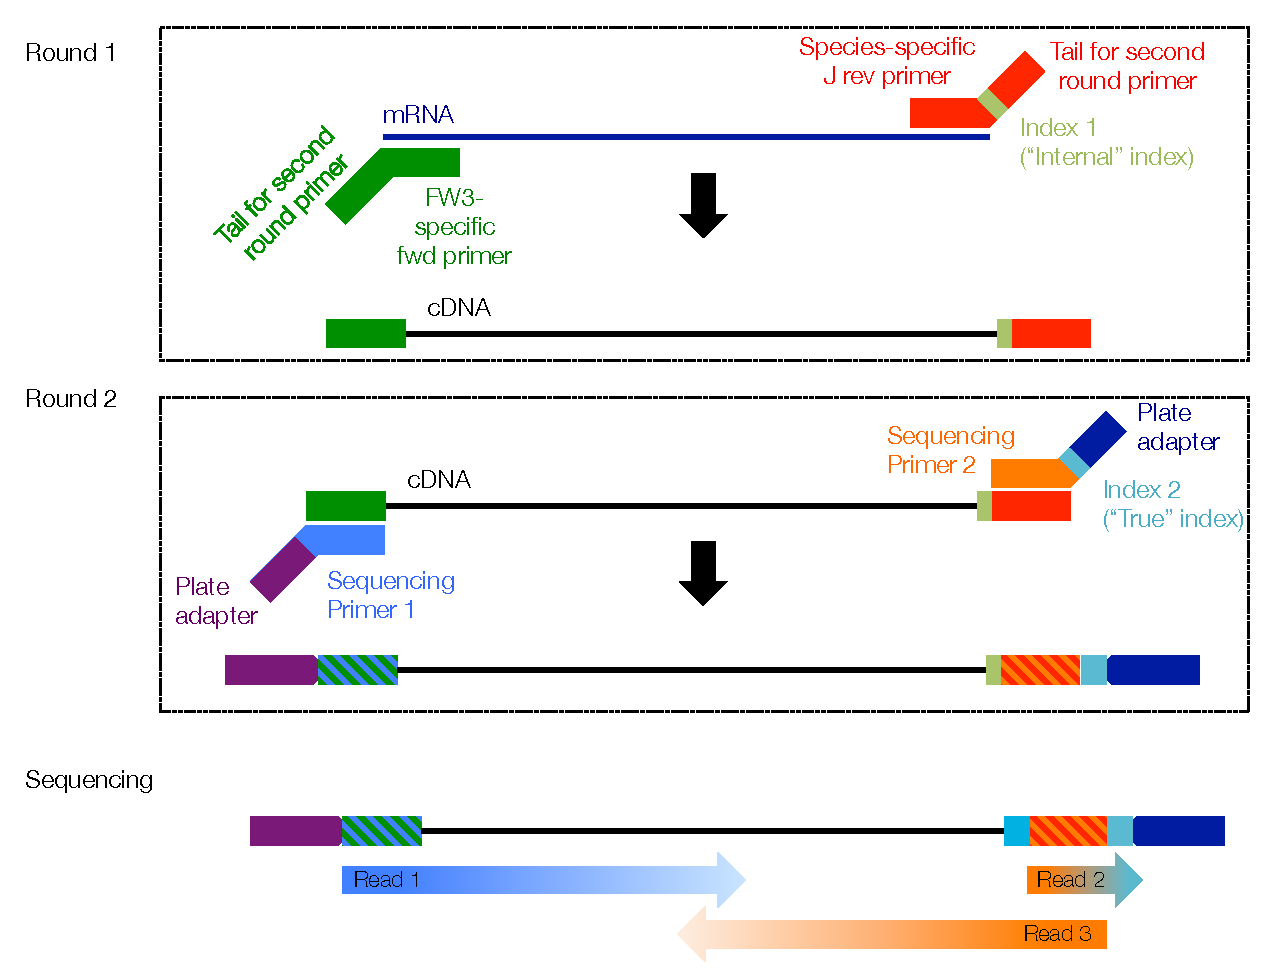
\includegraphics[width=.9\linewidth]{images/chapter3/figure3_6.pdf} % requires the graphicx package
% %    \caption[Current Sequencing Technologies]{Current sequencing technologies. On the x-axis is the current read length for each sequencing platform. The y-axis is the bases per run. Each point is a new iteration of that platforms sequencing read length and coverage. HiSeq has the most coverage with relatively short read lengths. Figure adapted from \citep{developmentinNGS:2012bs} }
% %    \label{fig:figure3_6}
% % \end{figure}

% % \begin{figure}
% %    \centering
% %    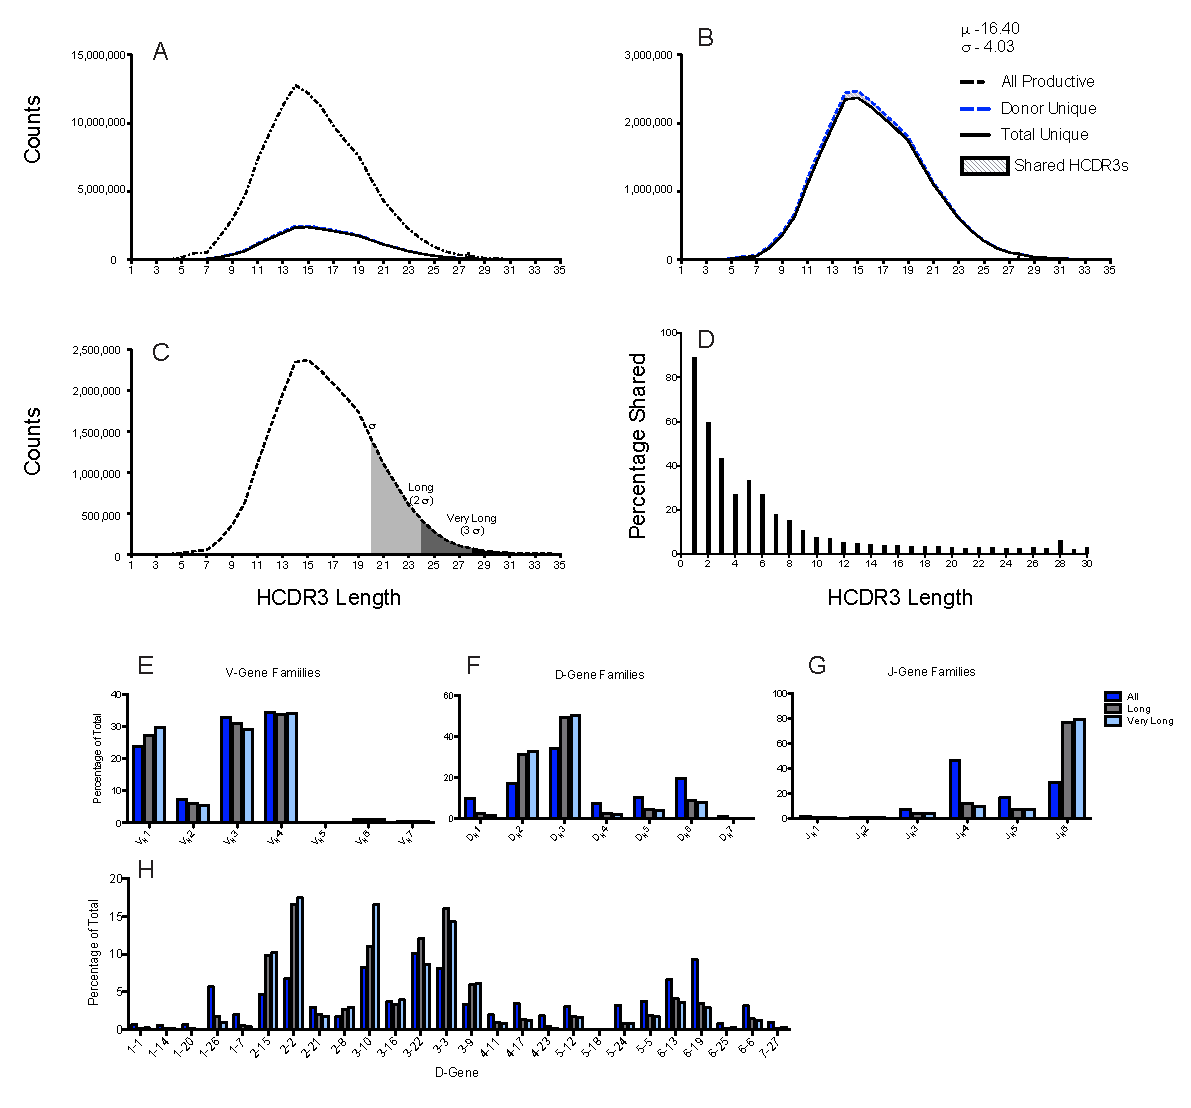
\includegraphics[width=.9\linewidth]{images/chapter3/figure3_7.pdf} % requires the graphicx package
% %    \caption[Current Sequencing Technologies]{Current sequencing technologies. On the x-axis is the current read length for each sequencing platform. The y-axis is the bases per run. Each point is a new iteration of that platforms sequencing read length and coverage. HiSeq has the most coverage with relatively short read lengths. Figure adapted from \citep{developmentinNGS:2012bs} }
% %    \label{fig:figure3_7}
% % \end{figure}

% % \begin{figure}
% %    \centering
% %    \includegraphics[width=.9\linewidth]{images/chapter3/figure3_8.pdf} % requires the graphicx package
% %    \caption[Current Sequencing Technologies]{Current sequencing technologies. On the x-axis is the current read length for each sequencing platform. The y-axis is the bases per run. Each point is a new iteration of that platforms sequencing read length and coverage. HiSeq has the most coverage with relatively short read lengths. Figure adapted from \citep{developmentinNGS:2012bs} }
% %    \label{fig:figure3_8}
% % \end{figure}

% % \begin{figure}
% %    \centering
% %    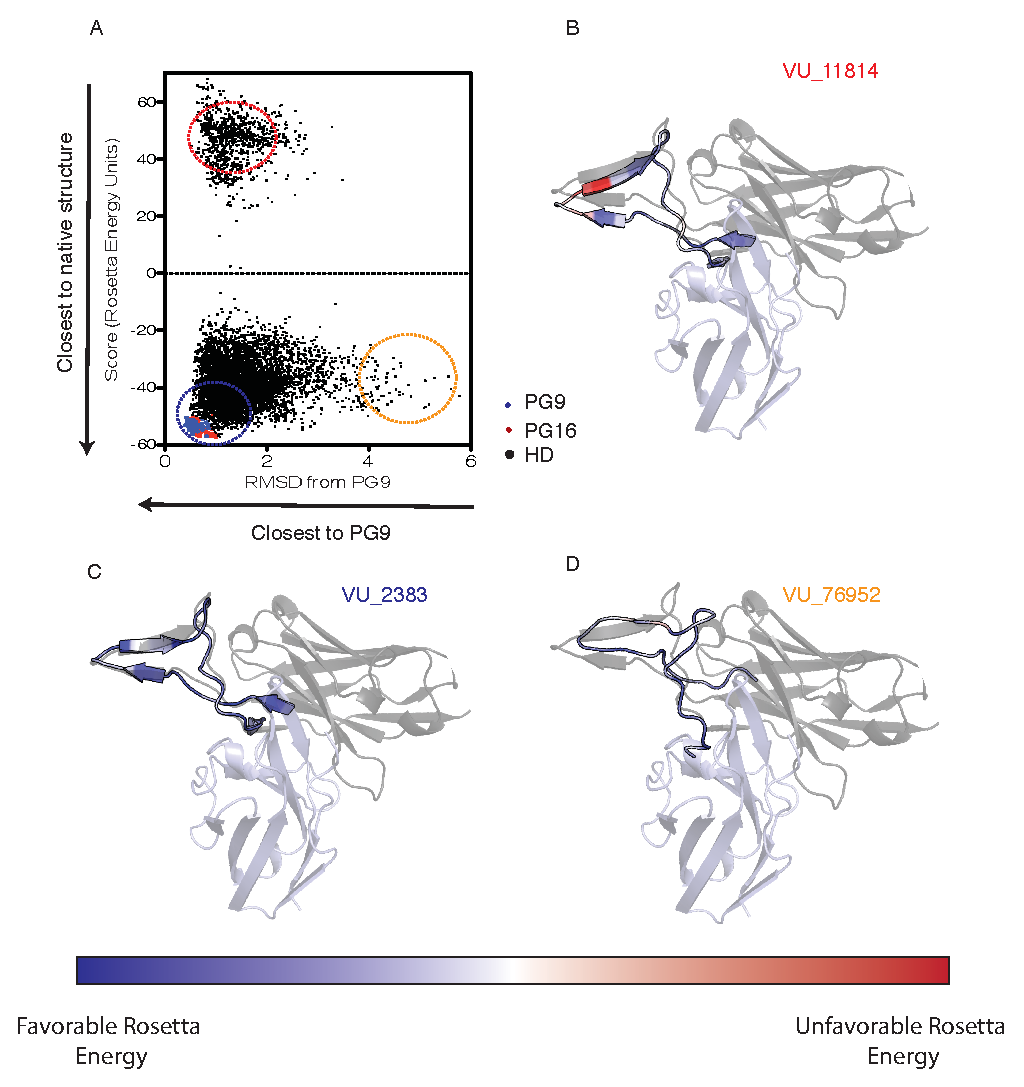
\includegraphics[width=.9\linewidth]{images/chapter3/figure3_9.pdf} % requires the graphicx package
% %    \caption[Current Sequencing Technologies]{Current sequencing technologies. On the x-axis is the current read length for each sequencing platform. The y-axis is the bases per run. Each point is a new iteration of that platforms sequencing read length and coverage. HiSeq has the most coverage with relatively short read lengths. Figure adapted from \citep{developmentinNGS:2012bs} }
% %    \label{fig:figure3_9}
% % \end{figure}

% % \begin{figure}
% %    \centering
% %    \includegraphics[width=.9\linewidth]{images/chapter3/figure3_10.pdf} % requires the graphicx package
% %    \caption[Current Sequencing Technologies]{Current sequencing technologies. On the x-axis is the current read length for each sequencing platform. The y-axis is the bases per run. Each point is a new iteration of that platforms sequencing read length and coverage. HiSeq has the most coverage with relatively short read lengths. Figure adapted from \citep{developmentinNGS:2012bs} }
% %    \label{fig:figure3_10}
% % \end{figure}

% % \begin{figure}
% %    \centering
% %    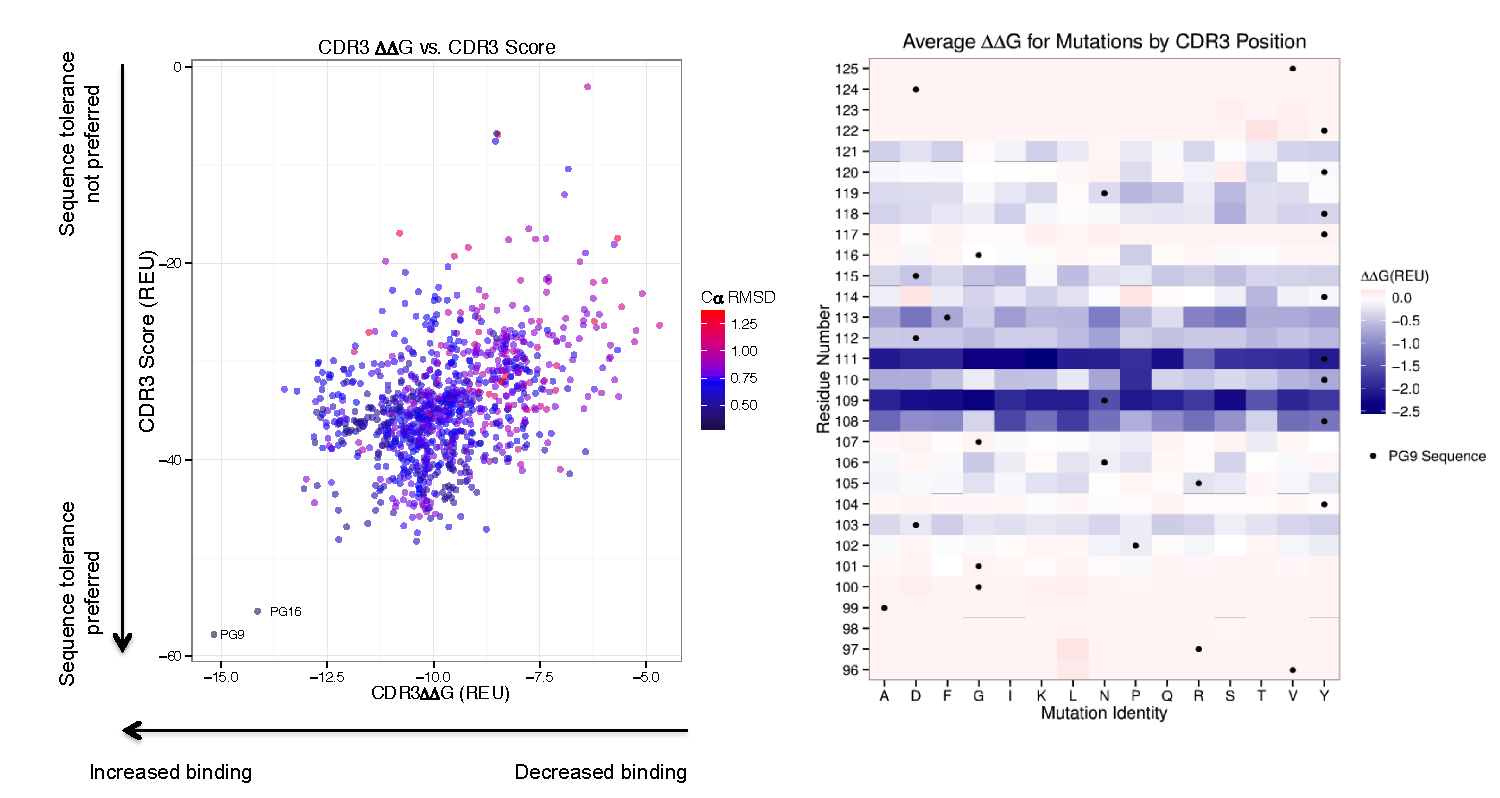
\includegraphics[width=.9\linewidth]{images/chapter3/figure3_11.pdf} % requires the graphicx package
% %    \caption[Current Sequencing Technologies]{Current sequencing technologies. On the x-axis is the current read length for each sequencing platform. The y-axis is the bases per run. Each point is a new iteration of that platforms sequencing read length and coverage. HiSeq has the most coverage with relatively short read lengths. Figure adapted from \citep{developmentinNGS:2012bs} }
% %    \label{fig:figure3_11}
% % \end{figure}

% % \begin{figure}
% %    \centering
% %    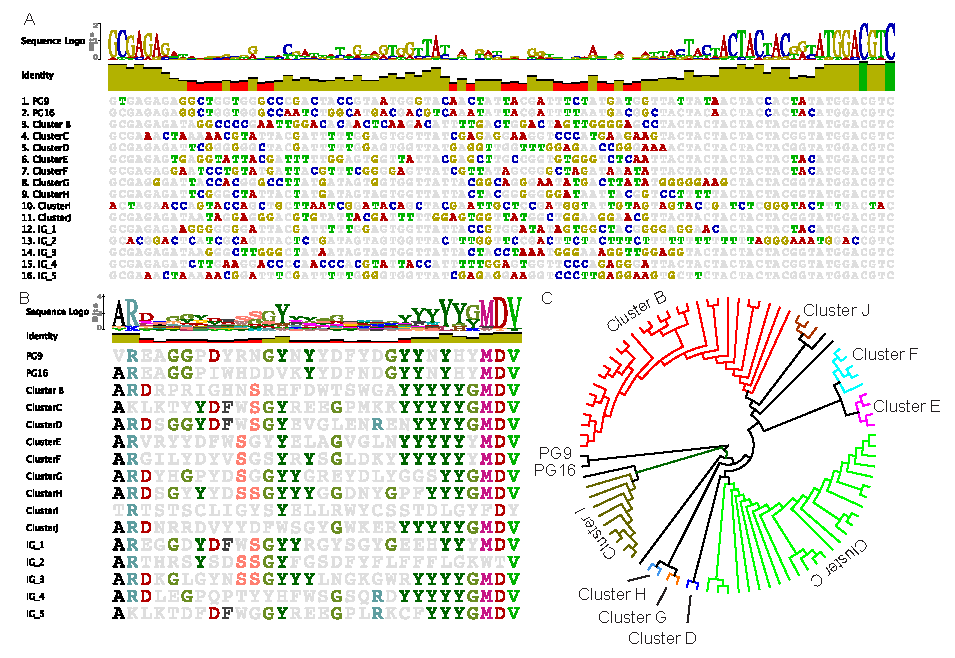
\includegraphics[width=.9\linewidth]{images/chapter3/figure3_12.pdf} % requires the graphicx package
% %    \caption[Current Sequencing Technologies]{Current sequencing technologies. On the x-axis is the current read length for each sequencing platform. The y-axis is the bases per run. Each point is a new iteration of that platforms sequencing read length and coverage. HiSeq has the most coverage with relatively short read lengths. Figure adapted from \citep{developmentinNGS:2012bs} }
% %    \label{fig:figure3_12}
% % \end{figure}

% % \begin{figure}
% %    \centering
% %    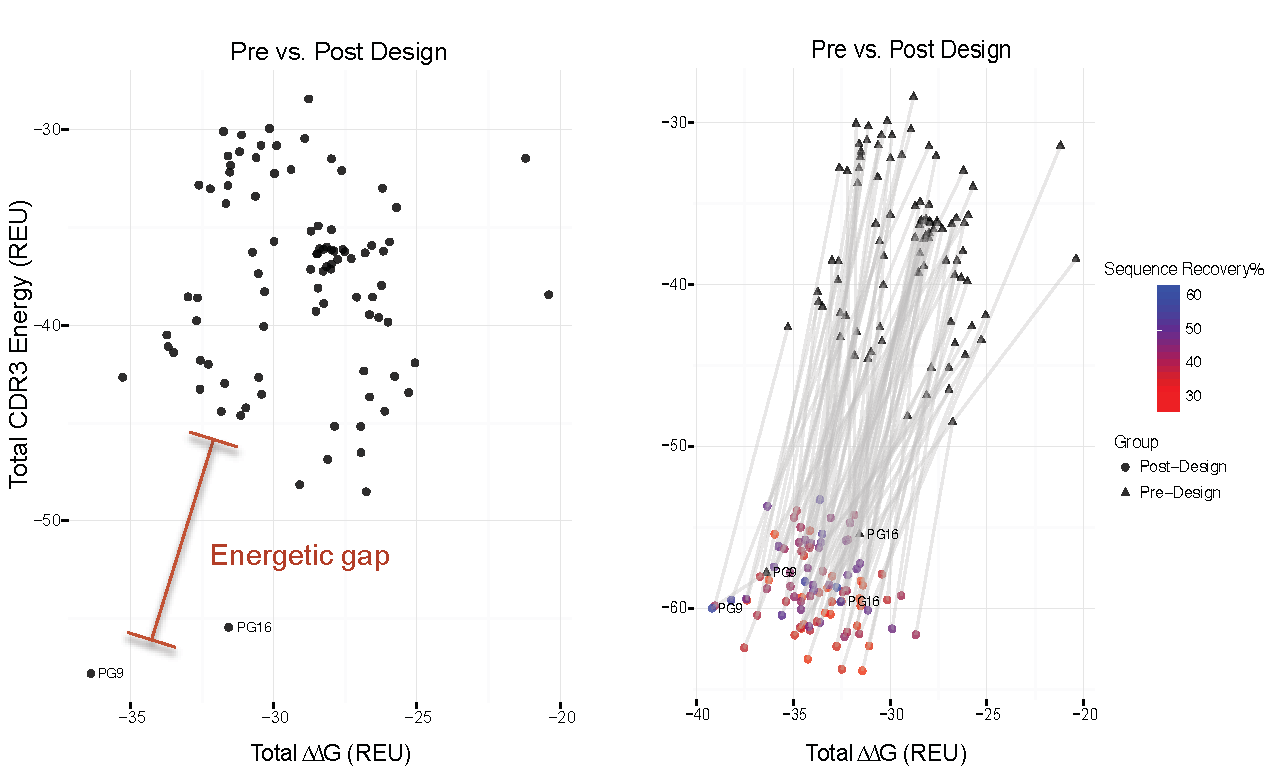
\includegraphics[width=.9\linewidth]{images/chapter3/figure3_13.pdf} % requires the graphicx package
% %    \caption[Current Sequencing Technologies]{Current sequencing technologies. On the x-axis is the current read length for each sequencing platform. The y-axis is the bases per run. Each point is a new iteration of that platforms sequencing read length and coverage. HiSeq has the most coverage with relatively short read lengths. Figure adapted from \citep{developmentinNGS:2012bs} }
% %    \label{fig:figure3_13}
% % \end{figure}

% % \begin{figure}
% %    \centering
% %    \includegraphics[width=.9\linewidth]{images/chapter3/figure3_14.pdf} % requires the graphicx package
% %    \caption[Current Sequencing Technologies]{Current sequencing technologies. On the x-axis is the current read length for each sequencing platform. The y-axis is the bases per run. Each point is a new iteration of that platforms sequencing read length and coverage. HiSeq has the most coverage with relatively short read lengths. Figure adapted from \citep{developmentinNGS:2012bs} }
% %    \label{fig:figure3_14}
% % \end{figure}

% % \begin{figure}
% %    \centering
% %    \includegraphics[width=.9\linewidth]{images/chapter3/figure3_15.pdf} % requires the graphicx package
% %    \caption[Current Sequencing Technologies]{Current sequencing technologies. On the x-axis is the current read length for each sequencing platform. The y-axis is the bases per run. Each point is a new iteration of that platforms sequencing read length and coverage. HiSeq has the most coverage with relatively short read lengths. Figure adapted from \citep{developmentinNGS:2012bs} }
% %    \label{fig:figure3_15}
% % \end{figure}

% % \begin{figure}
% %    \centering
% %    \includegraphics[width=.9\linewidth]{images/chapter3/figure3_14.pdf} % requires the graphicx package
% %    \caption[Current Sequencing Technologies]{Current sequencing technologies. On the x-axis is the current read length for each sequencing platform. The y-axis is the bases per run. Each point is a new iteration of that platforms sequencing read length and coverage. HiSeq has the most coverage with relatively short read lengths. Figure adapted from \citep{developmentinNGS:2012bs} }
% %    \label{fig:figure3_16}
% % \end{figure}


% % \begin{figure}
% %    \centering
% %    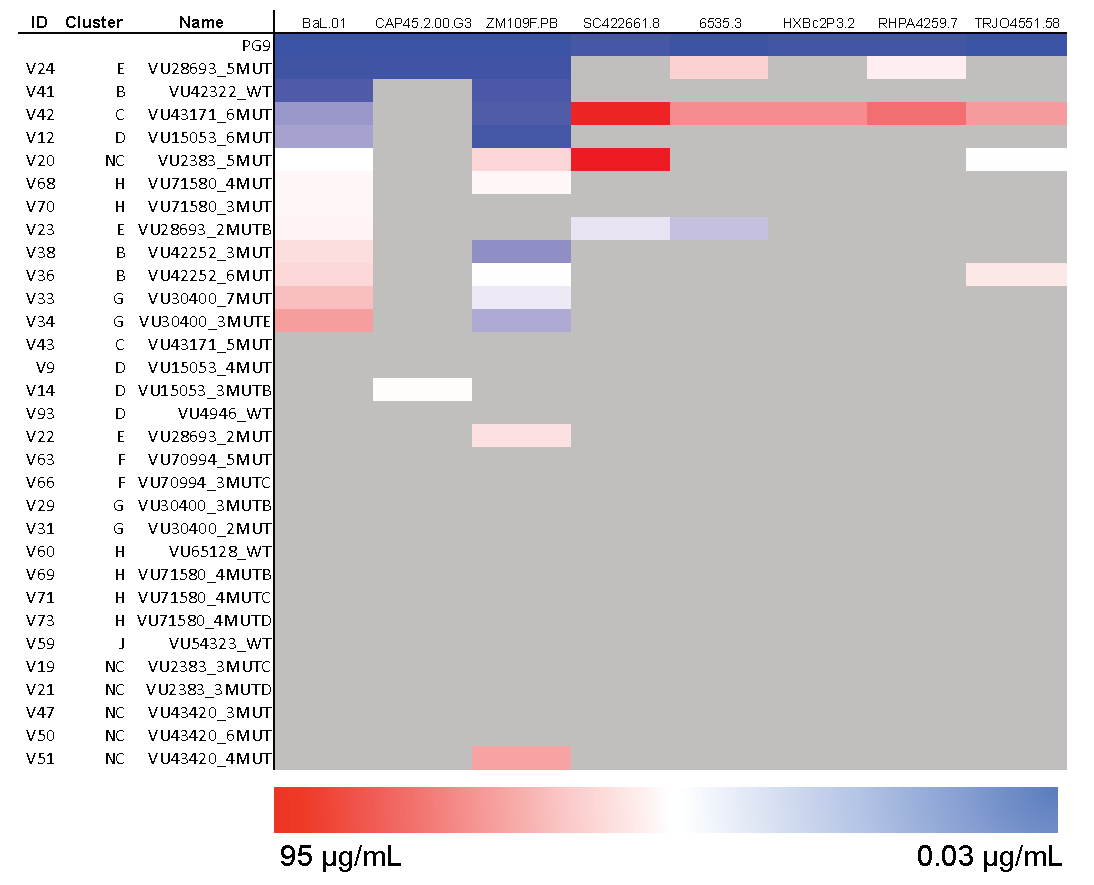
\includegraphics[width=.9\linewidth]{images/chapter3/figure3_17.pdf} % requires the graphicx package
% %    \caption[Current Sequencing Technologies]{Current sequencing technologies. On the x-axis is the current read length for each sequencing platform. The y-axis is the bases per run. Each point is a new iteration of that platforms sequencing read length and coverage. HiSeq has the most coverage with relatively short read lengths. Figure adapted from \citep{developmentinNGS:2012bs} }
% %    \label{fig:figure3_18}
% % \end{figure}

% %TABLES


% %
% %\begin{table}[!h]
\centering
\begin{tabular}{lc}
\textbf{Cluster}   & \textbf{Weighted Z-Score} \\
\hline
Cluster B & -1.24            \\
Cluster C & 0.28             \\
Cluster D & 0.11             \\
Cluster E & 0.15             \\
Cluster F & -0.34            \\
Cluster F & -0.20            \\
Cluster G & 0.31             \\
Cluster H & 0.11             \\
Cluster I & -2.54            \\
Cluster J & 1.48             \\
PG9       & -4.80            \\
PG16      & -1.87            \\
IG 4      & -1.46
\end{tabular}
\caption[Weighted Scores of PG9-Mimic Clusters]{Weighted scores of PG9-mimic clusters. Each cluster with the top scoring sequence is shown with weighted Z-score.}
\label{tab:table3_4}
\end{table}
% %\begin{sidewaystable}
\centering
\resizebox{.99\linewidth}{!}{
\begin{tabular}{cccccc}
\toprule
\textbf{Cluster} & \textbf{Total Candidates} & \textbf{Wild-Type Expressed$^{1}$} & \textbf{Mutants Expressed$^{2}$} & \textbf{Wild-Type Bound$^{3}$} & \textbf{Mutants Bound$^{4}$} \\ \hline
B                & 6                         & +                             & 5/5                         & ++                        & 3/5                     \\
C                & 5                         & ++                            & 3/4                         & -                         & 2/3                     \\
D                & 7                         & +++                           & 6/6                         & +++                       & 4/6                     \\
E                & 7                         & -                             & 6/6                         & N/A                       & 3/6                     \\
F                & 6                         & -                             & 2/5                         & N/A                       & 2/2                     \\
G                & 8                         & +++                           & 7/7                         & -                         & 4/7                     \\
H                & 7                         & +++                           & 4/6                         & +++                       & 4/4                     \\
I                & 6                         & -                             & 0/5                         & N/A                       & 0/0                     \\
J                & 6                         & +++                           & 4/5                         & +++                       & 1/4                     \\
IG               & 26                        & +                             & 23/25                       & -                         & 8/23                    \\ \hline\hline
\textbf{Total}   & \textbf{84}               & \textbf{7/10}                 & \textbf{60/74}              & \textbf{4/7}              & \textbf{31/60}         
\end{tabular}}
\captionsetup{singlelinecheck=off}
\caption[Expression and Binding Statistics]{Expression and binding statistics. Each cluster is shown with it's total number of candidates that we attempted expression and binding. We record if the wild-type sequence expressed and bound, as well as the number of mutant sequences that expressed and bound.
\begin{description}
		\item[Wild-type expression$^{1}$]: +-> 300 $\mu$g/L, ++ - > 1 mg/L, +++ - > 5 mg/L
		\item[Number of expressed mutants$^{2}$]. Positive if they expressed > 300 $\mu$g/L
		\item[Wildtype binding$^{3}$]: + -> 1 OD, ++ -> 2OD, +++ - > 3OD
		\item[Mutants bound$^{4}$]: Positive if OD > 1.0
\end{description}}
\label{tab:table3_5}
\end{sidewaystable}
%\chapter{Redesign of A Long HCDR3 Antibody}
\label{chap:chapter4}
\section{Introduction}
Recent studies described the isolation of a number of human monoclonal antibodies (mAbs) with broad and potent neutralizing activity, many of which exhibit unusual features \citep{Bonsignori:2011dq,McLellan:2011dg,Walker:2009cd,Walker:2011ew}. As discussed in the chapter \ref{chap:chapter1}, broadly neutralizing antibodies to HIV generally contain high levels of somatic mutations or exceptionally long HCDR3 lengths. The V2/V3 neutralizing class of anti-HIV antibodies which includes PG9, PG16, CH01, CH04, PGT141 and PGT145 all have a long heavy chain complementarity determining region 3 (HCDR3) and possess unique structural elements that interact with complex protein and glycan features reaching past a large bulk of complex and high mannose glycans to interact with a short segment termed strand-C5. These antibodies share similar neutralization sensitivity including glycan knockouts and strand-C point mutations that interact with interface residues \citep{DoriaRose:2012if,Doores:2010gn}.  For PG9 and its clonally related sibling PG16, crystal structures have been solved in complex with V1/V2 gp120 showing that these antibodies both engage the epitope with their HCDR3 loop in a similar ways with the exception of glycan interactions \citep{Pancera:2013ev}. While PG16 prefers hybrid type glycans at position N173 (HIV variant HXBc2 numbering), PG9 has little dependence.

\subsection{Experimental Rationale}
As an extension of my work in chapter \ref{chap:chapter3} that considers antibodies with exceptionally long HCDR3s, I chose to pursue a redesign study of the broadly neutralizing antibody PG9. This allowed me to ask relatively simple questions that may have broad and far-reaching implications for antibody and vaccine design. Is the native sequence of PG9 optimal for binding and neutralization potency? PG9 and PG16 converge on structure and binding modes but they are encoded by different sequences. Therefore, I hypothesized that the HCDR3 loop of PG9 could be redesigned to achieve improved affinity of binding, increased potency, and breadth of neutralization for diverse HIV strains.

There has already been precedent for chimeric antibodies of PG9/PG16 where a motif from PG16 responsible for the recognition of complex type glycans was transposed onto PG9 in order to increase potency and breadth. This approach allowed PG9, which initially had no preference for complex type glycans at position 173 (HIV variant HxBC2), to bind those glycan types with stronger affinity, while retaining PG9s ability to bind high mannose type antibodies. This chimeric antibody extended the breadth of PG9 with a small subset of mutations on the light chain CDR3 loop termed PG9-RSH \citep{Pancera:2013ev}.

In addition, NIH45-46, a broadly neutralizing mAb that shows structural mimicry for CD4 and closely resembles VRC01, was mutated by one amino acid in the HCDR2 loop \citep{Scheid:2011js,Diskin:2011hl}. The mutation was not designed computationally; rather, the investigators aligned the bound structure of NIH45-46 with CD4 and observed that CD4 had a hydrophobic burial of a phenylalanine residue at position 54 (figure \ref{fig:figure4_1} A). This interaction was recapitulated in another antibody, VRC03, with a tryptophan residue at position 54. The wild-type amino acid G54 did not fully recapitulate the CD4 interaction as it left a large gap between the gp120 outer domain and the HCDR2 (figure \ref{fig:figure4_1} A). The investigators predicted that a mutation to either a hydrophobic residue, such as the phenylalanine of CD4, or the tryptophan used by VRC03 would increase potency by increasing the mimicry of CD4. Indeed, a mutation to tryptophan at position 54 (NIH45-46\textsubscript{G54W}) increased neutralization potency for a majority of the viral strains tested and up to 2,000-fold for one of the strains (figure \ref{fig:figure4_1} B,C).

Using the high-throughput sequencing data obtained in chapter \ref{chap:chapter3}, I predicted I could map the energy landscape of the HCDR3 structure using the \rosetta~scoring function. That is, we sought to look at amino acid sequences at all positions of the HCDR3 and determine their overall level of fitness for each position. Does PG9 contain the optimal sequence for the HCDR3 loop? If I didn't see a complete recovery of PG9 sequence, I could then predict that other sequence combinations or point mutations exists that enhance fitness of the HCDR3 and may increase breadth and potency to HIV. Again, these mutations would then be carried over to the laboratory to be tested experimentally with binding and neutralization assays.

\begin{figure}
   \centering
   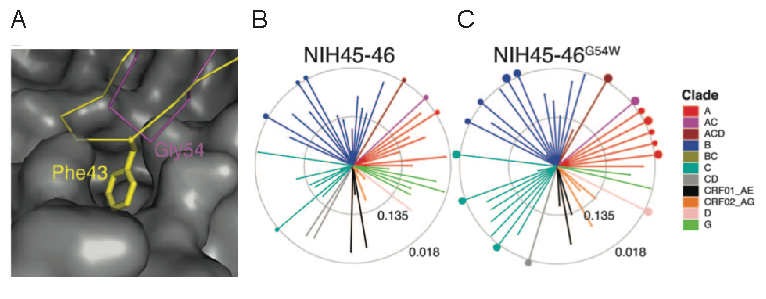
\includegraphics{images/chapter4/figure4_1.pdf} % requires the graphicx package
   \caption[Rational Design of NIH45-46 to Increase Neutralization Potency]{Rational design of NIH45-46 to increase neutralization potency. The gp120 bridging sheet is shown as a surface representation with CD4 shown in yellow and NIH45-46 shown in purple (A). Spider plots showing the neutralization profile for NIH45-46 and point mutant NIH45-46G54W are shown. The length of the line corresponds inversely with the \ic~value. Each circle represents a ten-fold change in \ic~(B,C). Figure adapted from \citep{Diskin:2011hl}}
   \label{fig:figure4_1}
\end{figure}

\section{Mapping the Energy Landscape of PG9}
\label{sec:mapping}
I retrieved the atomic resolution structure of the complex of mAb PG9 with the CAP45.2.00.G3 variant V1/V2 scaffold from the Protein Data Bank (PDB ID:3U4E) \citep{McLellan:2011dg}. A large number of naturally-occurring 30-amino-acid (30 AA) length HCDR3 antibody sequences was identified in antibody gene repertoires from high-throughput sequencing of antibody amplicons from RNA of B-cells of HIV-negative donors. Retrieval of this dataset is discussed at great length in chapter \ref{chap:chapter3}. A heat map of amino acid occurrences is displayed in figure \ref{fig:figure4_2} A for 30-length HCDR3s. Diversity among the repertoires is seen for all positions 98-118. The sequence conservation at the 5' and 3' ends of the HCDR3 sequences, 96-98 and 118-125, respectively, are due to the ARD motif that make up the 5' end of a canonical neck of a long HCDR3 loop or the J\textsubscript{H}6 template sequence, which was seen in a majority of long HCDR3 sequences \citep{North:2011dv,Briney:2012ib}. Between these two stretches of sequence conservation, I observed large sequence diversity. Glycine, tyrosine and serine are generally tolerated at all positions, while proline, lysine and methionine are found less frequently between positions 99-117 (figure \ref{fig:figure4_2}A). This phenomenon is well established in loop unstructured regions connecting beta-sheets in antibodies \citep{Minuchehr:2005wc,De:2005in}.  This propensity for a structure to tolerate a diverse set of amino acid sequences was the focus of the current study. The idea is that there is tremendous sequence space to be explored in 30-length HCDR3s that may further enhance breadth and specificity.

My methods are described fully in the appendix \ref{sec:appendixIII}, but use the same general protocol as described in Chapter \ref{chap:chapter3}. I used the software suite \rosetta~to determine the ability of diverse 30-AA HCDR3 sequences to tolerate the structure of the hammerhead configuration of the HCDR3 of PG9 by threading 4,000 naturally-occurring unique sequences over the PG9 HCDR3 structure. Once the sequences are threaded, I scored them by evaluating the \rosetta~scoring function for each position. The contribution to the total score of each position (the sum of all scoring terms of \rosetta), which can be thought of as thermal stability, and the contribution to the binding energy (the total score in complex subtracted from the total score in a separated interface) of each position were evaluated. These scores are best viewed as heat maps (figure \ref{fig:figure4_2} B,C). These two metrics, total score and binding energy, can be summed to determine what I define as the mutational ``fitness''. In this way, I trimmed the tremendous sequence space as viewed in the heat map in figure \ref{fig:figure4_2} A, to a focused sequence space containing mutations that advantageously affect either thermal stability or binding energy. These metrics are shown in the heat maps of figure \ref{fig:figure4_2} A-B, offer an advantage structure-based metrics in exploring design. As expected, PG9 itself scored as the most fit sequence for a majority of amino acid positions for the HCDR3 (dots plotted in figure \ref{fig:figure4_2}).

\begin{figure}
   \centering
   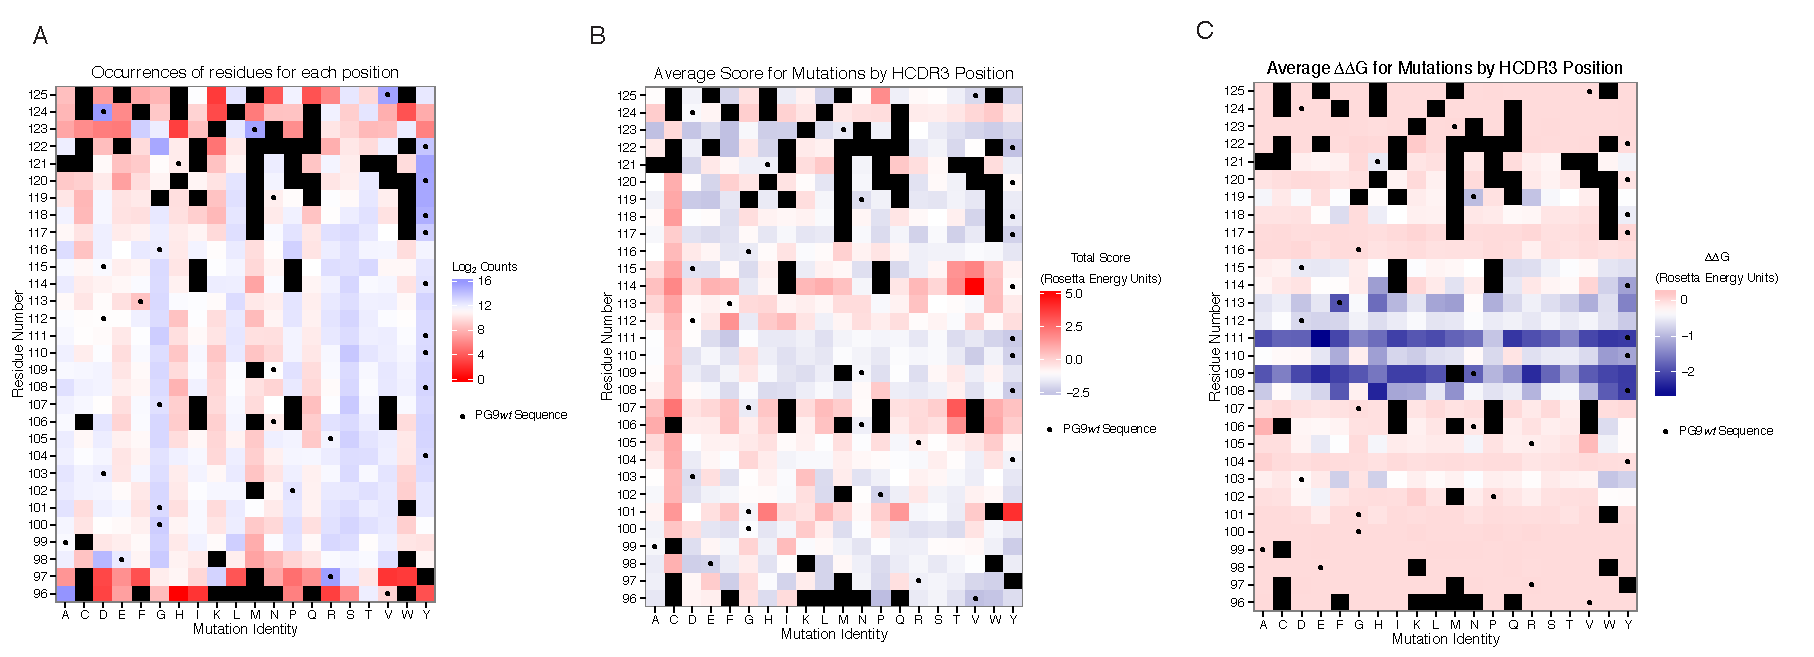
\includegraphics[width=.99\textwidth]{images/chapter4/figure4_2.pdf} % requires the graphicx package
   \caption[Amino Acid Usage and Energy Landscape of PG9]{Amino acid usage and energy landscape of PG9. Mutation identity is plotted on the x-axis with each of the positions in the 30-length HCDR3 on the y-axis. The usage of each amino acid is shown in a log\textsubscript{2} blue-red scale counted from 26,422 HCDR3 sequences (A). 4,000 randomly selected sequences were chosen and their individual score from the \rosetta~energy function is shown on a blue-white scale (B). The contribution of the same 4,000 randomly selected sequences contribution to binding energy is shown on a blue-white scale (C). For A-C, the PG9 native sequence is shown as a dot.
}
   \label{fig:figure4_2}
\end{figure}

\section{Redesign of PG9}
Rather than pick the amino acids that had the best fitness for each position, I allowed a complete redesign of the PG9 HCDR3 loop using \rosettadesign. My reasons for choosing this method rather than a simple matrix lookup generated in the previous section were two fold:
\begin{enumerate}
\item Complete redesign can account for cooperative mutations. Consider position 99 that has a wild-type alanine for PG9. My heat maps for the energy landscape predicted that there are many more favorable mutations I could make including an aspartic acid, asparagine or tyrosine. However, I are unaware if the new mutations have the potential to be cooperative. That is, do the aspartic acid, asparagine, or tyrosine require neighboring mutations to be fully stable? The complete redesign allowed me to account for cooperative mutations while recapitulating the energy landscape predicted in section \ref{sec:mapping}.
\item Using a combination of filters and movers based on my specific design goals, I prevented \rosetta~from designing amino acids too far away from the original PG9 sequence, position, and structure. I can also tell the \rosetta~scoring function to optimize for binding energy, thermal stability, or a combination thereof. This information would be lost on a matrix lookup \citep{Fleishman:2011ji,Kaufmann:2010ea,Kuhlman:2000tc}.
\end{enumerate}

Again, the full design protocol is detailed in the in the Appendix (Chapter \ref{sec:appendixIII}) and follows the same basic structure as the redesign of sequences detailed in Chapter \ref{chap:chapter3}. I designed 1,000 decoys allowing small docking perturbations and minimal backbone movement. I filtered the design to optimize for binding energy. That is, only obtain sequences if they were better than binding energy of PG9\textit{wt}.

The easiest way to view the sequences returned from the PG9 redesign is with a sequence logo representation (figure \ref{fig:figure4_3} A). The x-axis is the PG9\textit{wt} sequence while the height of the letters at each position, measured in bit, measure \rosetta's preference for that amino acid given the nature of the design challenge. As expected from the observations from the energy landscape (figure 4.2), the original PG9 sequence was returned for a majority of the positions, considering the evolutionary sequence bias of the PG9 structure (nature optimizes sequences for the PG9 structure).  Regardless, anytime an amino acid was returned in 10\% or more of the models, I further inspected the design fitness of the mutation.

I measured the design fitness as a sum of the difference in total energy from wild-type sequence and the difference in binding energy from the wild-type sequence ($\Delta\Delta$G + total score). For some of the positions, multiple amino acids were suggested by \rosetta~rather than the wild-type amino acid sequence (figure \ref{fig:figure4_3} A,B). For most positions, the design fitness was negligible, falling above the noise threshold (figure \ref{fig:figure4_3} B, dashed-line). However design at antibody amino acid positions 104, 109, 115, 120, and 123 (PDB numbering) suggested alternative amino acids that were predicted to benefit HCDR3 fitness for the antibody-V1/V2 interaction (figure \ref{fig:figure4_3} B).

I wanted to make sure that each of these mutations made intuitive sense upon examination of the structure. I viewed each mutation in context and compared it to the wild-type amino acid. My aim was to determine if this mutation was an artifact and to confirm that it was non-cooperative with other mutations, that is, the mutation enhances fitness alone and not in cooperation with many other mutations made to the sequence. This is because I wanted to retain as much of the PG9\textit{wt} sequence as possible. These visual inspections are shown in figure \ref{fig:figure4_3} B in the table, with a full justification given. If a mutation was found to be non-cooperative, and still enhanced fitness, it was considered for experimental characterization (green squares), N109Y and D115N met these criteria. I also considered N109L and a cooperative mutation A99S and Y120N as they showed strong stabilization through inter-HCDR3 loop hydrogen bonding. I also made one combinatorial mutation that included the double cooperative mutant A99S-Y120N and two single mutations D115N and N109L. This variant is simply referred to as PG9\_4MUT (figure \ref{fig:figure4_3}C). I did not pursue further evaluation of designs that appeared to compromise the structural integrity of the HCDR3 loop by visual inspection.

\begin{figure}[!t]
   \centering
   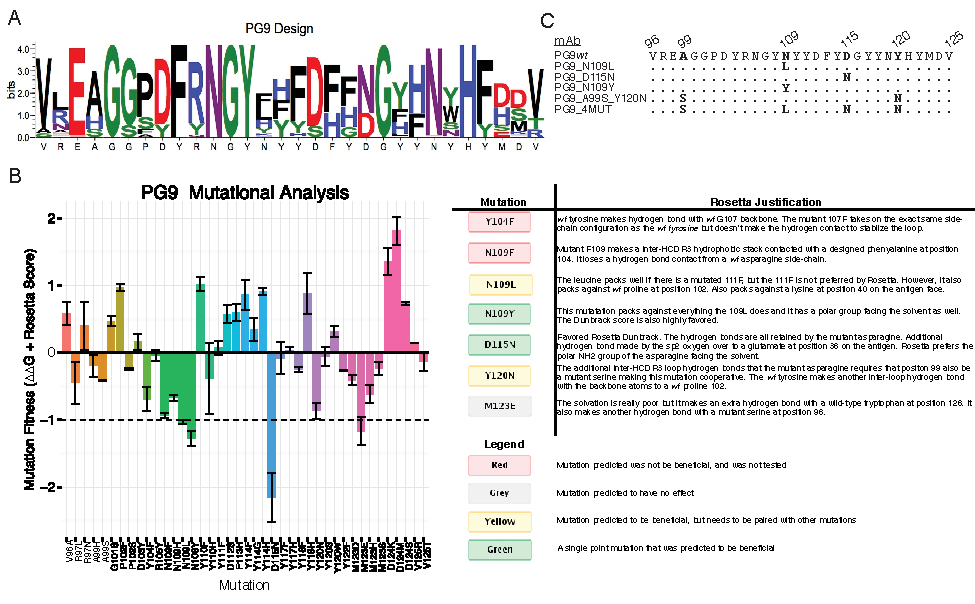
\includegraphics[scale=1.5,width=.99\textwidth]{images/chapter4/figure4_3.pdf} % requires the graphicx package
   \caption[Redesign of PG9 HCDR3]{Redesign of PG9 HCDR3. For 1,000 designed models, the sequences returned are best viewed as a sequence logo. The x-axis is the PG9\textit{wt} sequence while the y-axis represents the preference, measured in bit, of the amino acid identities, identified by the height of the letter (A). For sequences that were returned greater than 10\% of the time, I manually inspected their fitness as a measure of binding energy and thermal stability (y-axis). Some positions had more than one amino acid favored and are grouped by color. \rosetta~noise is plotted as a dashed line at -1 REU. The more negative a mutation is, the more it is beneficial to the PG9 complex. Each mutation is visually inspected and justified (table). They are either a single point mutations that benefits, a cooperative mutation that benefits, no change in fitness, and detriment to fitness, as green, yellow, grey, and red, respectively (B). The final mutations that are chosen to be carried out experimentally are three point mutations and two combinations thereof (C).}
   \label{fig:figure4_3}
\end{figure}


\section{Experimental Characterization of PG9 Variants}
For the five mutational variants of PG9, I used a similar cloning strategy as described in Chapter \ref{chap:chapter3} that takes advantage of unique cloning sites between the HCDR3 5' and 3' ends. Each of the variants expressed well, and protein concentration was not a limiting factor. I began by testing all the variants against a 15 antigen mix of gp120 Env proteins to qualitatively measure binding. In this preliminary study, the double mutant, A98S-Y120N produced a significantly lower signal than that of PG9, and this variant was not considered further.

PG9\textit{wt} does bind to some gp120 monomers (although PG9\textit{wt} also can neutralize HIV variants for which it does not bind to monomer). I used a panel of representative gp120 monomers from HIV clades B and C to perform screening for binding of PG9 variants to Env \citep{Li:2006kv,Li:2005go}. The results were in good agreement with previous studies of the binding of PG9\textit{wt} to gp120 monomers \citep{McLellan:2011dg}. For these PG9 variants, I calculated half-maximal effective concentration (\ec) values. For each gp120 monomer tested, the PG9 variants N109L and N109Y exhibited 2.3-14.2 fold stronger binding than did PG9\textit{wt} (figure \ref{fig:figure4_4}), while PG9 variant D115N exhibited comparable binding energies to PG9\textit{wt}. PG9\_4MUT exhibited 2-100 fold reduced binding. This finding is most likely due to the A98S-Y120N mutation that I had previously determined as deleterious.

I also determined the \ec for binding of these PG9 variants to a recombinant form of native gp140 trimer that is recognized by PG9, termed BG505-SOSIP.66419-21. In these assays, both PG9 variants N109L and N109Y exhibited 3.5- or 5.9-fold stronger binding respectively than PG9\textit{wt}. In addition to the stronger binding affinity, the variant N109Y bound to trimer with a complete sinusoidal curve and a strong maximum signal mimicking the binding profile of the glycan-specific mAb 2G12, which is optimal for binding to the trimer \citep{Sanders:2013gm}  (figure \ref{fig:figure4_4}A). The extreme change in maximal signal is intriguing, and may suggest changes in valency of P9 to the trimer although this has not been confirmed \citep{Julien:2013jp}.

I next tested the panel of redesigned PG9 variants and PG9\textit{wt} for neutralizing activity against a panel of viruses displaying PG9-susceptible or -resistant HIV Env molecules, using a TZM-bl neutralization assay \citep{Montefiori:2009hj}. The PG9 variant N109Y exhibited increased neutralization potency for all viruses tested, including viral variants for which PG9\textit{wt} did not have activity (i.e., had neutralization concentration >33 \mcml) (figure \ref{fig:figure4_4}B). Remarkably, PG9 variant N109Y neutralized at 3.72 \mcml~an HIV strain with the N160A mutation that removes the glycan at that position that is required for binding of PG9\textit{wt}6. The PG9 variant N109L also exhibited an increase in potency against HIV strains compared to PG9\textit{wt}, although not at the same level as the PG9 variant N109Y. In all assays tested, N109Y and N109L consistently had enhanced breadth and potency.

The magnitude of the improvement to neutralization was modest in some cases, but the improvement was consistent over a wide variety of HIV strains and showed significant p-values (p < 0.05) for 10 out of the 15 virues for PG9\_N109Y and 4 out of the 15 viruses for N109L (table \ref{tab:table4_1}). Using a meta-analysis for all p-values tested gave a p-value of 5.44 x 10\textsuperscript{-15} and 7.36 x 10\textsuperscript{-4} indicating a strong statistical significance observed for the increase in potency of neutralization for PG9\_N109Y and PG9\_N109L respectively. I also found a decrease in potency to be statistically significant for 8 out of the 15 viruses tested for PG9\_D115N and a combined p-value of 2.64 x 10\textsuperscript{-8}.


\begin{figure}[!t]
   \centering
   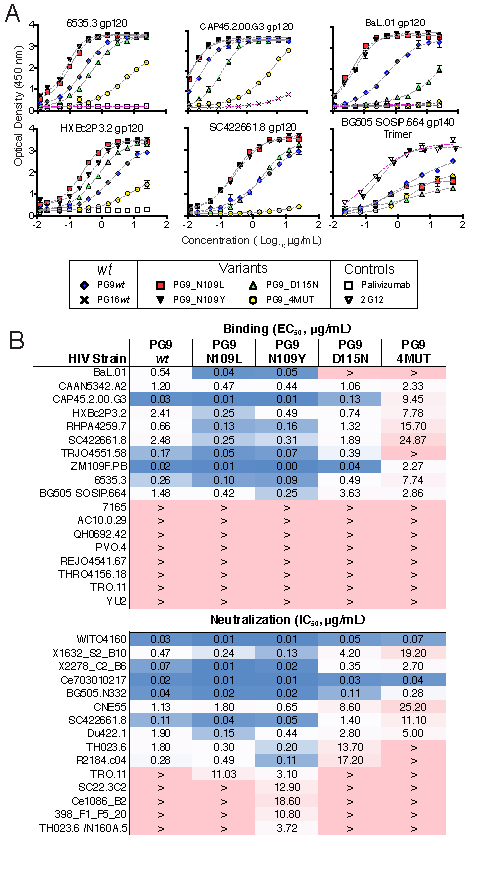
\includegraphics{images/chapter4/figure4_4.pdf} % requires the graphicx package
   \caption[Experimental Analysis of PG9 Variants]{Representative binding curves are shown with the optical density at 450 nm shown on the y-axis plotted against the log\textsubscript{10} concentration in \mcml~on the x-axis (A). All \ec values were calculated from the curves like the ones shown in (A) as well as the neutralization \ic~against a 15 virus panel (B)}
   \label{fig:figure4_4}
\end{figure}

\begin{table}[!t]
    \centering
    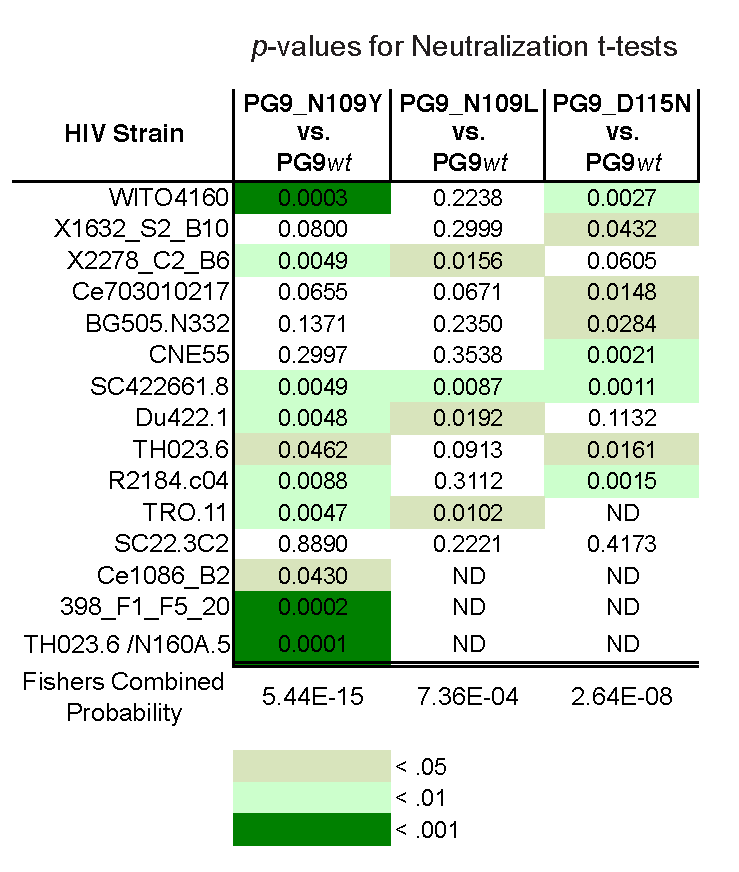
\includegraphics[scale=.8]{tables/chapter4/table4_1.pdf}
    \caption[Statistical Tests for Neutralization Breadth of PG9 Variants]{Statistical tests for neutralization breadth of PG9 variants. The \ic~values between each neutralization assay for PG9\_N109Y, PG9\_N109L, and PG9\_D115N were compared with a student's non-parametric t-test against the \ic~value for PG9. They are shown as p-values for each viral variant. A total p-value for each antibody is shown as a Fisher's combined probability.}
    \label{tab:table4_1}
\end{table}


\section{Models to Corroborate Experimental Outcome}
I sought to develop a predictive model to determine the molecular basis for the increased potency and breadth of these PG9 variants using the \rosetta~scoring function. I generated three different mutants D115N, N109L and N109Y, which were compared to that of PG9\textit{wt} using the \rosetta~scoring function (figure \ref{fig:figure4_5} A). I analyzed the top 25 models for each of the scoring metrics shown. my scoring metrics were binding contribution for the HCDR3, binding for the full complex, total score for the bound and unbound structure ($\Delta\Delta$G). For each metric calculated, I observed statistically significant improvements in HCDR3 stabilization for N109L or N109Y (p < 0.01 or p < 0.001, respectively), but none of my other metrics.

Upon examination of the predicted structures of the top scoring models, I found the antibody position 109 was located on an antiparallel beta-sheet at the apical tip of the HCDR3 forming a hydrophobic pocket near the interface of the antigen and apical tip (figure \ref{fig:figure4_5} B). The pocket is formed by antibody residues Y104, Y110 and P102 of the antibody heavy chain (PDB numbering). In addition, D167 on the antigen face makes contact with this position. Examination of the structure revealed that the bulk of the hydrophobic amino acid at this position of the pocket contributes to stabilization of the preferred structure of HCDR3. The small hydrophobic bulk of the asparagine fills the pocket, but as the bulk increased to a leucine and then a tyrosine, the predictive model suggested a further stabilization of the HCDR3 loop. In addition, the polar group on the end of the designed tyrosine at position 109 points into solvent space, recapitulating the effect of the polar head of the original asparagine PG9\textit{wt}t.

It is important to note that since I calculate the stabilization as the total energy of the HCDR3 loop, it can be dissected into the individual scoring terms given by \rosetta. These are both described in the chapters \ref{chap:chapter1} and the appendix \ref{chap:appendix}. I have broken the total score down for the HCDR3 loop in figure \ref{fig:figure4_6}. There is little deviation for most of the scoring terms, however, both the attractive force term, the solvation term in the \rosetta~scoring function are improved for the N109L and N109Y mutations. In addition the N109Y shows a favored $\pi$-$\pi$ term. These interactions are accounted for in the model as the N109 position is between a large hydrophobic bulk. In addition, position N109Y also achieves a more favorable $\pi$-$\pi$ stacking interaction with residue Y110 compared to PG9\textit{wt} as the aromatic ring of the designed tyrosine can stack with position 110.

\begin{figure}[!t]
   \centering
   \includegraphics[width=.99\textwidth]{images/chapter4/figure4_5.pdf} % requires the graphicx package
   \caption[Predictive Models of PG9 Variants that Enhanced Binding]{The top 25 models for each binding metric are analyzed. The x-axis is each of the variants and the y-axis is the \rosetta~energy units. The metrics are decomposed by binding energy (A) and thermal stabilization (B). Just the HCDR3 is considered (left) or the entire complex (right). Surface representation of position 109. Green is the antigen labeled V1/V2, blue is the HCDR3 loop, dark green is the N160 glycan. Each mutation of interest is shown as a sphere representation that is adjusted to fit the \rosetta~ atom radius. Spheres are colored by atom type with oxygen in red, nitrogen blue, and carbon in grey. Hydrogens are removed for clarity.}
   \label{fig:figure4_5}
\end{figure}


\begin{figure}[!t]
   \centering
   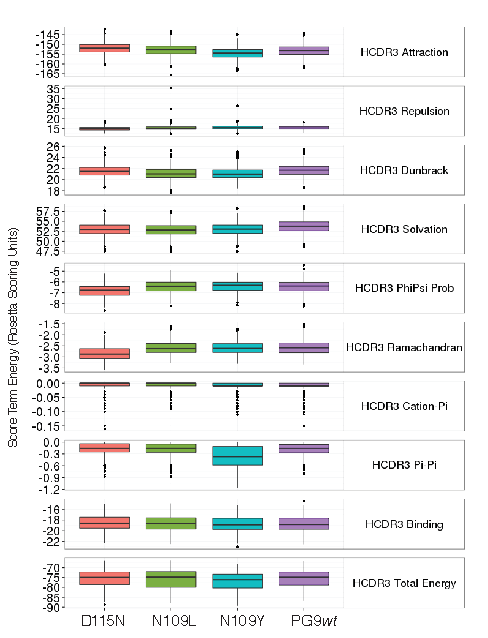
\includegraphics[scale=1.4]{images/chapter4/figure4_6.pdf} % requires the graphicx package
   \caption[Decomposed Scoring Terms for PG9 Variants]{Decomposed scoring terms for PG9 variants. The contribution of individual scoring terms to the total energy score for the HCDR3 loop for each mutation. The predictive model used 1000 simulations for each variant. Each scoring term for \rosetta is shown in the y-axis panel. The y-axis value is the score for that energy term.}
   \label{fig:figure4_6}
\end{figure}


\section{Discussion}
These results have important implications for antibody and vaccine design. The studies reveal the power of \rosetta~computational modeling to design antibodies with improved function using structural predictions. Remarkably, the improvements in neutralizing potency and breadth observed here for PG9 variants were achieved not by altering interface residues, but rather by increased stability of HCDR3 loops discovered using a holistic model to determine stability of an antigen-antibody complex. This finding is consistent with recent mutagenesis experiments showing that non-contact residues are essential for antigen recognition by many broadly neutralizing antibodies to HIV \citep{Klein:2013iz}. Non-contact residues in antibody frameworks contribute to high affinity binding by facilitating formation and stability of a pre-configured, low energy binding site \citep{Willis:2013dd,Manivel:2000wk,Marlow:2010jl,Wedemayer:1997wn,Schmidt:2013ka}. Optimally configured binding sites form ordered paratopes that pay a smaller entropic penalty upon forming antibody-antigen complexes \citep{Marlow:2010jl}.

This work shows the efficiency of combining \rosettadesign~computational experiments with expert knowledge and wet laboratory validation experiments. For a HCDR3 loop of 30-AAlength, 600 single point mutants are possible, and the number of variants with more than one mutation is enormous. From this large potential set of mutated antibodies, \rosettadesign~identified a focused panel of candidate PG9 variants, from which a small subset was considered favorable, and two of five experimentally tested variants exhibited enhanced potency and breadth of neutralization. The computational experiments provided tremendous enrichment for variants with improved binding, but as expected was not completely accurate. For example, although the model suggested that D115N would have the greatest increase in fitness (figure 4.3) this variant was not improved in activity.
The negative result is important, as \rosetta~often predicts design failures, and their exploration is fundamental in improving the \rosetta~algorithm and scoring function for the most accurate representations of experimental observation. This computational-experimental feedback has been instrumental to my work and will be the target of my future directions.

With the combination of high-throughput sequencing, rapid threading, and experimental feedback, I complete a robust bioinformatics pipeline that can rapidly test antibodies for improvement based solely on their \silico~predictions. The results here suggest that there probably is a diversity of antibodies with long and structured HCDR3s that fit the PG9 topology in nature with HIV neutralizing activity that have yet-to-be discovered. I hypothesize this conclusion from three parts of evidence:
\begin{enumerate}
\item Examination of the energy landscape of PG9 suggests that there are mutations that are predicted to be better suited for the PG9 topology.
\item PG9 and PG16 diverge in sequence but converge on a structural topology and have approximately identical specificities and potencies \citep{McLellan:2011dg,Pejchal:2010fp,Pancera:2010hh}.
\item I have discovered point mutations in PG9 that enhance breadth and specificity.
\end{enumerate}
These yet to be discovered antibodies may possess higher HIV inhibitory activity and breadth than the antibodies that are currently in hand. Additional antibody exploration efforts may be worthwhile to identify antibodies of interest with which to design epitope mimetic vaccines, as has been successfully recently implemented \citep{Correia:2014jp,Jardine:2013hb}.



\section{Conclusions and Future Directions}
Two observations may be critical to explore in this current work. The maximum signal difference in the binding assay for the BG505-SOSIP trimer between my variants and the PG9\textit{wt} is worth further exploration. Julien and colleagues observed that PG9 recognizes the trimer asymmetrically \citep{Julien:2013jp}. There are three epitopes displayed on the apical tip of the gp120 trimer, yet PG9 only has a 1:3 valency of binding to HIV Env. The molecular mechanism for this trimeric preference is unavailable due to the high resolution of the structure reported in the study, but the model suggests that PG9 may interact with the adjacent N160 glycan. Could the mutation cause a change in valency in binding? This change would explain to the maximal signal change in my binding assay. Future experiments could replicate the study performed by Julien \textit{et al.} either with high-resolution gel-filtration or isothermal titration calorimetry.

Another observation is the glycan independence of the binding of the N109Y variant. It was originally thought that the binding of any V1/V2 binding antibody would depend on glycans at position N160 and N156/N1706 considering they not only block the recessed C-strand epitope, but make considerable binding contributions for both PG16 and PG9 \citep{McLellan:2011dg,Pancera:2013ev}. It was demonstrated that these glycans are needed for recognition and specificity, as mutational experiments completely abrogated neutralization. I was able to replicate that finding, however, my variants still neutralized HIV glycan knockout viruses, albeit, at much lower potency (3.52 \mcml). It is worth replicating this ``glycan independence'' with many more viral species that have been mutagenized to knockout glycans. I have already begun to pursue this aim.

Finally, I can attempt to repeat the application of this entire technology to mutagenesis of PG9's sibling, PG16. I already have the mutational candidates, and the antibody cDNAs are being synthesized at the time of this writing. It is important to keep in mind that PG16 specific to the trimeric-Env, so variants can only be tested with neutralization experiments or if I synthesize stable trimer \citep{Sanders:2013gm}.





\chapter{Conclusions and Future Directions}
\label{chap:chapter5}
\section{Chapter \ref{chap:chapter1}}
% \chapter{Appendix}
\label{chap:appendix}
%appendix I
\section{Appendix I - \rosetta~Glossary}
\label{sec:appI}
\singlespace
\setlength{\parindent}{0pt}

\textbf{All-atom} - in the case of sampling, synonymous with fine movements and often including side chain information; also referred to as high-resolution \\ \\

\textbf{Benchmark} - another word for a test of a method, scoring function, algorithm, etc. by comparing results from the method to accepted methods/models \\ \\

\textbf{Binary file} - a file in machine-readable language that can be executed \textit{in silico} \\ \\

\textbf{BioPython} - a set of tools for biological computing written and compatible with Python \\ \\

\textbf{Build} - to compile the source code so it may be used as a program \\ \\

\textbf{Centroid} - in \rosetta centroid mode, side chains are represented as unified spheres centered at the residues center of mass \\ \\

\textbf{Cluster center} - the geometric center of a cluster, or group, of models \\ \\

\textbf{Clustering} - in this case, grouping models with similar structure together \\ \\

\textbf{Comparative model} - a protein model where the primary sequence from one protein (target) is placed, or threaded, onto the three dimensional coordinates of a protein of known structure (template) \\ \\

\textbf{Cyclic coordinate descent (CCD)} - based on robotics, CCD loop closure is used to build loops in \rosetta by fragment assembly and close loops by decreasing the gap between two termini in three-dimensional space \\ \\

\textbf{\textit{De novo}} - from the sequence; also called \textit{ab initio}, with no experimental guidance \\ \\

\textbf{Directory} - synonymous with a folder, usually contains one or more files or other folders \\ \\

\textbf{distance matrix} - a matrix containing the pairwise distances for every point in a set of points \\ \\

\textbf{Dunbrack rotamer library} - a set of likely side chain conformations for the twenty canonical amino acids based on protein structures in the Protein Data Bank (PDB) \\ \\

\textbf{Executable} - binary file used to execute the program \\ \\

\textbf{Force field/Scoring function/Energy function/Potential} - often used interchangeably; a means of assessing the energy of the generated models \\ \\

\textbf{Fragment} - in \rosetta folding and loop building, a set of three-dimensional coordinates corresponding to a given amino acid sequence fragment \\ \\

\textbf{Database} - also called the fragment library, contains all the interchangeable data needed for \rosetta \\ \\

\textbf{Gap} - in sequence alignment, a gap is inserted when the sequences are of low homology; usually appear as a dash (-); the gaps form a sequence alignment correspond to areas where loops are
built during comparative modeling \\ \\

\textbf{GDT/GDT\_TS} - global distance test (total score); a measure of similarity between two protein structures having the same amino acid sequence; the largest set of residues C$\alpha$ atoms in the model structure falling within a defined distance cutoff of their position in the experimental structure \\ \\

\textbf{Gradient-based minimization} - also known as minimization by steepest descent; in this case, a means of energy minimization in which one takes steps proportional to the negative of the gradient of the function (energy) at the current point \\ \\

\textbf{High-resolution} - in the case of sampling, synonymous with fine movements and often including side chain information \\ \\

\textbf{Homology model} - a more specific type of comparative model where the protein sequence of interest (target) is a homolog of the protein of known structure (template) \\ \\

\textbf{Interface delta} - the interface delta score is defined as the contribution to the total score for which the presence of the ligand is responsible \\ \\

\textbf{Kinematic loop closure (KIC)} - robotics-inspired loop closure algorithm which analytically determines all mechanically accessible conformations for torsion angles of a peptide chain using polynomial resultants \\ \\

\textbf{Knowledge-based} - in the case of \rosetta, based on information obtained from structures found in the PDB \\ \\

\textbf{Libraries} - in computing, a collection of code and data (classes and functions) used by a piece of software and is often used in software development \\ \\

\textbf{Ligand} - the part of the structure that binds to a protein to serve some biological purpose \\ \\

\textbf{Low-resolution} - a somewhat subjective term, in the case of sampling, synonymous with coarse movements of the protein and/or ligand backbone and side chains; the individual atoms of low-resolution structures or models cannot be resolved, or observed \\ \\

\textbf{Metropolis criterion} - often combined with the Monte Carlo sampling algorithm; allows for generation of an ensemble that represents a probability distribution \\ \\

\textbf{Model} - in the case of this protocol, a structure generated by \rosetta; sometimes called a decoy \\ \\

\textbf{Monte Carlo sampling} - a randomized and repetitive computational sampling method \\ \\

\textbf{Mover} - a generic class that takes as input a pose and performs some modification on that pose; for example, a mover might take in a pose and rotate every residue \\ \\

\textbf{Namespace} - in computer science, an abstract container holding a logical grouping of unique identifiers or symbols; in \rosetta, examples of namespaces are loops, relax, etc. \\ \\

\textbf{Native-like} - close to the experimentally determined structure; a model that is native-like usually has an RMSD to the experimentally determined structure of < 2\r{A} \\ \\

\textbf{Options file} - often called a flags file; a file containing \rosetta options that can be passed to a \rosetta executable after the @ symbol; can be easier to use than passing \rosetta options over the command line \\ \\

\textbf{Pack/repack} - in \rosetta, side chains are packed/repacked by switching out rotamers and scoring them using the \rosetta scoring function \\ \\

\textbf{Pose} - in  \rosetta protocol, a three-dimensional conformation of the ligand, protein, or ligand/protein complex at any given time-point \\ \\

\textbf{Python} - interpreted, object-oriented, high-level programming language \url{http://www.python.org/} \\ \\

\textbf{Relax} - in \rosetta, an iterative protocol of side chain repacking and gradient-based minimization; often referred to as full-atom (or all-atom) refinement \\ \\

\textbf{Robetta}  \rosetta structure prediction server (\url{http://robetta.bakerlab.org/}) freely available to not-for-profit users \\ \\

\textbf{RosettaCommons} - a group of more than twenty labs that develop the \rosetta software suite  \\ \\

\textbf{REU} - arbitrary energy units specific to the \rosetta scoring function \\ \\

\textbf{RosettaScripts} - also called ``the scripter'' or RosettaXML; an XML-like language that allows for specifying modeling tasks in \rosetta \\ \\

\textbf{Rotamer} - rotational conformer of an amino acid or ligand side chain \\ \\

\textbf{SCons} - a tool for constructing software from its source code \url{http://www.scons.org/} \\ \\

\textbf{Script} - in computer programming, a script is a sequence of instructions that is interpreted or carried out by another program rather than by the computer processor (as a compiled program is) \\ \\

\textbf{Source code} - human-readable files that are the implementation of the program; are written in C++ in \rosetta \\ \\

\textbf{Target} - in comparative, or homology, modeling, the protein for which we are generating a model; the target sequence is the primary sequence of the protein for which we want to make a model \\ \\

\textbf{Template} - in comparative modeling, the protein of known structure on which the target is threaded \\ \\

\textbf{Threading} - placing the primary sequence of one protein (target) on the three-dimensional coordinates of a protein of known structure (template) based on a sequence alignment loop building \\ \\

\textbf{XML} - Extensible Markup Language; in this case, used to write protocols to pass to

\clearpage
\section{Appendix II - \rosetta~Scoring Terms}
%appendix II
\renewcommand{\arraystretch}{1.8}
\begin{table}[ht!]
\begin{tabular}{lp{11cm}}
\textbf{Scoring Term}      & \textbf{Explanation of Scoring Term}                                                                                         \\ \hline
Attraction                 & The Van de Walles scoring term to indicate how much attraction residues have on each other                                   \\
Dunbrack                   & A statistical probability score indicating how often a side-chain configuration has been seen in the protein data bank (PDB) \\
Repulsion                  & The Van De Walles scoring term to indicate how much repulsion residues have on each other                                    \\
Solvation                  & How well are hydrophobics packed away from solvent and hydrophillic groups are facing solvent                                \\
Ramachandran               & A statistical probability of how well $\phi$-$\psi$ angles fit into the Ramachandran plot as a function of secondary-structure     \\
Total                      & A summation of all individual scoring terms to get a total score                                                             \\
\ddg                       & The change in total energy score when residues are moved out of complex                                                      \\
$\phi$-$\psi$ Prob         & A statistical probability score of how well a side-chain configuration has been seen given a $\phi$-$\psi$ angle in the PDB  \\
Cation-$\pi$               & A score encompassing how the configuration of positive cation at the end of a charged reisidues interact with pi orbitals    \\
$\pi$-$\pi$                & A score encompassing how two $\pi$ orbitals interact                                                                            \\
HCDR3 Stabilization        & The total score of residues only found in the HCDR3                                                                          \\
Full Complex Stabilization & The total score of all residues representing a free energy of the model                                                      \\
HCDR3 Binding              & The contribution to \ddg by residues found in the HCDR3                                                                       \\
Full Complex Binding       & The \ddg for the entire complex
\end{tabular}
\caption[\rosetta~Scoring Terms]{}
\end{table}
\clearpage
\doublespacing
\section{Appendix III - Materials and Methods}
\label{sec:appendixIII}
\par\vspace{10pt}
\subsection{Chapter \ref{chap:chapter2} - Materials and Methods}
\par\vspace{10pt}
\subsubsection{Selection of Antigen-Antibody Complexes}
Diverse antigen-antibody complexes were collected from the Protein Data Bank (PDB; \url{www.pdb.org}) in which antibodies in different complexes were derived from the same predicted heavy chain variable gene segment. Candidate complexes were queried from the protein databank using the IMGT-3D structural query editor for immune system receptors \citep{Kaas:2004kv}. PDB structures were used as design candidates if they met the following criteria: 1) the antibody was encoded by a V\textsubscript{H}1-69, V\textsubscript{H}3-23, or V\textsubscript{H}5-51 gene segment, 2) the structure contained a human immunoglobulin, and 3) the ligand type was a protein complex. The search yielded 10, 8, or 3 antibody-antigen complexes encoded by the heavy chain variable gene segments V\textsubscript{H}1-69, V\textsubscript{H}3-23, or V\textsubscript{H}5-51, respectively. Nature of the antigen and antibody isotype were not considered in the selection as the 21 complexes represent an exhaustive search of the PDB for these gene-segments. The gene segments were aligned using the ClustalW2 multiple sequence alignment algorithm \citep{Larkin:2007hz}. Each input structure was energetically minimized using the \rosetta scoring function but constrained to PDB input backbone coordinates \citep{Das:2007em}.

\subsubsection{Multi-state Design of Antigen-Antibody Complexes}
Three design experiments were performed, one for each of the three germline segments (V\textsubscript{H}1-69, V\textsubscript{H}3-23, or V\textsubscript{H}5-51) using the multi-state design mode of the \rosetta algorithm and scoring functions. I adapted a generalized multi-state design protocol that was described in detail previously that perform design on multiple antibody-antigen complexes at once \citep{LeaverFay:2011ji}. Briefly, each computational design experiment computed an optimal sequence predicted to define a low-energy structure.  In the multi-state design experiments, an energetic consensus sequence for all of the states was predicted, rather than treating each state as a separate entity. The energy for a given sequence was computed and designated the ``design fitness'' for all states. The corresponding amino acids were derived from the alignment (\textit{e.g.}, heavy chain amino acid 5 on complex A corresponded to heavy chain amino acid 5 on complex B). The details of the multi-state algorithm is described elsewhere \citep{LeaverFay:2011ji}.

\subsubsection{Single-State Design of Antigen-Antibody Complexes}
Single-state design was performed using the \rosetta~multi-state application. The algorithm was altered so that only one complex was considered for each of the 10, 8, or 3 design experiments with V\textsubscript{H}1-69, V\textsubscript{H}3-23, or V\textsubscript{H}5-51 complexes, respectively.

\subsubsection{Design Analysis of Multiple- or Single-State Design}
For each design experiment, 100 independent design trajectories were calculated. Sequence logos then were generated using the Berkley web-logo server (\url{http://weblogo.berkeley.edu/})~\citep{Crooks:2004do}. Information for each sequence logo can be extrapolated as follows extending the work of Schneider \textit{et al.} \citep{Schneider:1990ub}. For each variable position, the probability of seeing each of the 20 naturally encoded amino acids p\textsubscript{i} was computed and compared with the background probability p\textsubscript{b} = 1/20 = 5\%. To quantify the deviation of the observed probability from the background probability I compute the self-information for each of the 20 amino acids as I\textsubscript{i} = p\textsubscript{i} x log\textsubscript{2}(20 x p\textsubscript{i}) in `bit'. If the amino acid occurs as often as expected from the background probability, I\textsubscript{i} is zero. Ii becomes larger if the amino acid is over-represented and approaches 4.32 if p\textsubscript{i} = 100\%. A total bit-score for the sequence design was obtained by summing all individual bit-scores for each amino acid. The bit-scores for the target sequence then were analyzed, and statistics were computed using Prism software version 5.0 (GraphPad Software).  For comparisons between germline sequence and mature sequence within the same design experiment, a Wilcoxon matched pairs test (non-normal, paired t-test) was used to compute the p-value at 99\% confidence level. For comparison between design experiments, a student's paired t-test was used to compute the p-value at 99\% confidence level.

\subsubsection{Amino Acid Environment}
The neighbor vector algorithm quantitatively determines the surface-exposure of a given residue and is described by Durham and colleagues elsewhere \citep{Durham:2009kt}. Briefly, each C$_{\beta}$ is computed to a vector and each vector is given a score based on the number and orientation of each C$_{\beta}$in the proximity. The weight of each neighbor falls of as a function of distance.
For interface scores, the change in neighbor vector was used, where the neighbor vector score of the amino acids in the unbound antibody is subtracted from the neighbor vector scores of the complex. Interface residues would have a large change in neighbors and proportional to the change in neighbor vector score.

\subsubsection{Phi-psi Angle Calculations}
All V\textsubscript{H} framework residues were grouped by complex. For each residue, phi-psi angles and secondary structure classification were determined using DSSP \citep{Kabsch:1983bp}. For each residue position across all complexes considered in design, the standard deviation of the phi-psi angles was calculated if they were included in the beta-sheet framework. A student's t-test was performed between the standard deviations between residue positions that recovered to germline (bit-score > 1), or did not recover to germline (bit-score < 1). For a reference, a deviation for all framework beta-sheet positions was also calculated for all residues even if they were not included in the design protocol.
\clearpage
\subsection{Chapter \ref{chap:chapter3} - Materials and Methods}
\par\vspace{10pt}
\subsubsection{RNA Extraction}
Peripheral blood mononuclear cells were isolated from 64 HIV-uninfected individuals (HIV-\naive) by processing leukoreduction filters as previously described \citep{Weitkamp:2001vm}. Briefly, RC2D leukoreduction filters were obtained from the American Red Cross and were backwashed with 35 mL of sterile PBS with 10mM EDTA. The resulting PBMC suspension was overlaid onto 15 mL of HistoPaque 1077 and centrifuged at 600 RCF for 25 minutes. The buffy coat was removed and washed twice with fresh PBS with 10mM EDTA. Total RNA was isolated from 10 million PBMCs using the RNeasy kit according to the manufacturer's standard operating procedure.

\subsubsection{cDNA Synthesis, PCR Amplification and Purification}
cDNA was synthesized from 100 ng of total RNA and 10 pmol of each RT-PCR Illumina-adapter primers in duplicate 50 \microliter~RT-PCR reactions using the OneStep RT-PCR system. The RT-PCR reactions were performed in a BioRad DNA Engine PTC-0200 thermal cycler running the following protocol: 50\degree C for 30:00, 95\degree C for 15:00, 35 cycles of (94\degree C for 0:45, 58\degree C for 0:45, 72\degree C for 2:00), 72\degree C for 10:00. cDNA synthesis was confirmed on a 1\% E-Gel EX. After which duplicate reactions were pooled. 2 \microliter~of each cDNA sample and 20 pmol of each indexed Illumina-adapter primer were used to template 100 \microliter~PCR amplification reactions in duplicate using the AmpliTaq Gold polymerase system. Thermal cycling was performed using the following protocol: 95\degree C for 10:00, 10 cycles of (95\degree C for 0:30, 58\degree C for 0:45, 72\degree C for 2:00), 72\degree C for 10:00. Amplicons were purified from the PCR reaction mix using the Agencourt AMPure XP system following the standard protocol, and duplicate reactions were pooled during the final elution. The removal of primers and correct amplicon size was confirmed on a 1\% E-Gel EX. Each amplicon sample was quantified using a Qubit fluorometer and the Quant-iT\textsuperscript{\textregistered} dsDNA HS Assay Kit and 8 indexed amplicon samples were pooled for each of the 8 lanes on the Illumina HiSeq flowcell.

\subsubsection{Illumina HiSeq Protocol}
The amplicon libraries underwent quality control by running on the Agilent Bioanalyzer High Sensitivity DNA assay to confirm the final library size and on the Agilent Mx3005P qPCR machine using the KAPA Illumina library quantification kit to determine concentration. For each library a 2 nM stock was created and denatured with NaOH. 12 pM of denatured libraries were loaded on the Illumina cBot for cluster generation on a paired-end flow cell. The flow cell was then loaded onto the Illumina HiSeq 2000 utilizing v3 chemistry and HTA 1.8. The raw sequencing reads in BCL format were processed through CASAVA-1.8.2 for FASTQ conversion and demultiplexing. The RTA chastity filter was used and only the pass filter reads were retained for further analysis.

\subsubsection{Paired-End Read Assembly and Junction Analysis}
FASTQ paired end reads were input into PANDAseq assembler software to produce a single sequence that was indexed by donor and position \citep{Bartram:2011cz}. Each sequence was uploaded to a custom database using the MongoDB framework that carried donor, position, sequence, and Phred quality score. The resulting sequences were concatenated and converted to FASTA format using BioPython SeqIO module \citep{Cock:2009hj}. Heavy chain CDR3 (HCDR3) junctions were analyzed using custom software. The software was modified to run in parallel on a high throughput computing cluster and to condense output to a minimum number of fields. The software was also modified to output the junction results in JSON format. The sequences were analyzed with BioPython to remove sequence ambiguity in each donor. The JSON files were then uploaded to the custom database using MongoDB framework. The two databases were linked by their donor id and position.

\subsubsection{30 Length HCDR3 Selection and Position Specific Structure Scoring Matrix (P3SM) Generation}
The custom database was queried for 30-length HCDR3 amino acid sequences generating > 26,000 unique sequences. 4,000 random sequences were selected for the pilot analysis in order to generate a custom position specific structure score matrix (P3SM) for PG9 HCDR3 structure. PG9 in complex with scaffolded template CAP45 (PDB ID: 3U4E) was used as a starting structure. The structure was stripped of waters and heavy chain and light chain constant regions. For the first round pilot, I also removed the CAP45 complex. Next, I used R\textsc{osetta}S\textsc{cripts} application available with the software suite from the R\textsc{osetta}C\textsc{ommons} (www.rosettacommongs.org) to thread and minimize the random HCDR3 sequences from HIV-\naive donors \citep{Fleishman:2011ji}. 50 decoys of each sequence were allowed to energetically minimize after threading yielding 200,000 models. 2,000 sequences (100,000 models) were used to fill the 30 by 20 P3SM using \rosetta per amino-acid energies of the HCDR3 loop. The remaining 2,000 sequences were used to benchmark the P3SM protocol.

\subsubsection{Selecting Sequences from the P3SM Heuristic for Validation}
After benchmark validation, the random 4,000 sequences were used in a final construction of a P3SM. Rapid prediction of score for each of the 26,000 HIV-\naive~HCDR3 sequences were calculated using the P3SM. PG9's sequence scored 112\textsuperscript{nd} out of 26,000 giving a noise tolerance of -3.82 REU (The top scoring sequence subtracted from the PG9 Score). Using $\pm$ 3.82 as my noise tolerance from PG9's score, 1,000 candidate sequences were selected to be further evaluated in complex.

\subsubsection{Sequence Tolerance Evaluated by Rosetta Design in Complex}
The top 1,000 candidate sequences evaluated by the P3SM were carried on to a separate \rosetta~protocol. This protocol evaluated sequence tolerance in complex with CAP45 antigen and surrounding glycans. N-linked glycan 156 and 160 (HXBC2 numbering) were both included in the complex input to \rosetta~as a non-canonical amino acid using the method described in Renfrew et al. \citep{Renfrew:2012ci}. After determining proper binding orientation with PG9, the entire complex was threaded with HIV-\naive~sequences. High-resolution docking perturbations were allowed but highly constrained to initial orientation using standard \rosetta~constraints files. I generated 100 models for each \naive~sequence and calculated a binding energy for each complex as:

\begin{gather*}
    \Delta \Delta \textup{G} = \Delta \textup{G}_{\textup{Bound}} - \Delta \textup{G}_{\textup{Unbound}} \\
    \textup{were,} \\
    \Delta \textup{G}_{\textup{Bound}} = \textup{RosettaScore}_{\textup{Complex}} \\
    \textup{and}\\
    \Delta \textup{G}_{\textup{Unbound}} = \textup{RosettaScore}_{\textup{Separated}}
\end{gather*}

In addition, the protocol was run a second time with sulfated tyrosines at positions 100G and 100H (Kabat numbering) if a tyrosine appeared at those positions in the HIV-\naive~sequences. Complex energies and interface binding metrics were parsed into a MySQL database for further analysis using included scripts from BioPython.

\subsubsection{Bootstrapping with Complex Energies}
The energy of each model evaluated in complex was reapplied to the P3SM and again ran through each HIV-\naive~donor sequence to predict a Rosetta energy using the same methodology as described. The bootstrapped models were included in the rest of the protocol.

\subsubsection{HIV-Na\"{i}ve Complex Energy Evaluation}
To filter \naive sequences into a realistic number to synthesize I evaluated multiple metrics. To weight each sequence, Z-Scores were assigned for the following score term metrics. HCDR3 total energy, HCDR3 C$\alpha$-RMSD, HCDR3 \ddg (the contribution to binding energy from just the HCDR3), total \ddg, ASN156 \ddg, and ASN158 \ddg. The Z-score is a measure of how many standard deviations a scoring metric fell from the mean. In terms of energy, all negative Z-Scores are preferred. When a Z-score was assigned for each HIV-\naive complex sequence, an average weighted Z-score was calculated using the following equation:

\begin{gather*}
\textup{Weighted-Z} = \frac{\sum_{i}^{N}w_{i}\times Z_{i}}{N}
\end{gather*}

Weights (w\textsubscript{i}) for each score term in the equation: total \ddg~-3.0, HCDR3 C$\alpha$-RMSD - 0.5, HCDR3-\ddg~-1.0, HCDR3 Score - 1.0, ASN156 \ddg~- 0.5, and ASN158 \ddg~- 0.5. This comprehensive metric can be used to rank-order each complex. In addition I used PG9 as a positive control and determined how many standard deviations away each of the HIV-\naive~complex scoring terms were from PG9's score using the following equation:
\begin{gather*}
\textup{Compare Score} = \frac{\bar{X}_{Scoring Term}-\bar{X}_{PG9 Scoring Term}}{\sigma_{PG9 Scoring Term}}
\end{gather*}

The compare score can then be weighted using the previous equation using the same weights to give one comprehensive metric to rank-order each HIV-\naive~sequence. The top 50 sequences were selected based on the average of the weighted compare score and weighted Z-score. 32 additional models were included from the bootstrapped protocol in the final results yielding 82 candidate HIV-\naive~sequences for experimental characterization.

\subsubsection{Clustering Analysis}
The sequences were clustered with ClustalW2 built in clustering algorithm after a multiple sequence alignment. The ClustalW plugin was used from the Genious Software suite (\url{http://www.geneious.com/}). The dendrogram was manually inspected and clusters were assigned yielding 10 candidate sequence groups for experimental characterization.

\subsubsection{Design Analysis for Sequence Tolerance}
Using the \rosettadesign~algorithm, the HIV-\naive~sequences tested for recovery using a small energetic bonus for favoring the native sequence \citep{Kuhlman:2000tc}. I applied a filter to minimize score and binding energy while favoring the native sequence. 100 models were generated using this protocol. After analysis, the sequence recovery was added to the Z-score metrics and the compare score using a weight of -2.0 (negative weight for favoring positive deviations) and reevaluated. Within each cluster, the HIV-\naive~sequence with the highest recovery and lowest Z-Score was further evaluated. For each mutated position, if a mutation was seen in greater that 10\% of the models and gave an energetic bonus of greater than 1.5 \rosetta~Energy Units (REUs), it was manually inspected using PyMOL and compared with the native sequence along with the native PG9 sequence from the native crystal complex (PDB ID: 3U4E).

\subsubsection{Antibody Expression}
To prepare HIV-\naive~PG9 variants and PG9 variant point mutations, I used recombinant expression in mammalian cells as previously described \citep{Xu:2010da}. Briefly, the MAb PG9 heavy- and light-chain genes were cloned into the pEE6.4 and pEE12.4 vectors, respectively. A BsiWI and XhoI cloning site were generated at AA position 95 and 110 (Kabat numbering), respectively. Using the unique cloning sites, the HIV-\naive~HCDR3 sequences were synthesized and cloned into the PG9 backbone. The DNA was co-transfected at a 1:1 heavy-light chain ratio into HEK 293F using polyethylenimine transfection reagent at a ratio 2:1 of PEI to DNA. 30 mL of culture was used for each variant and supernatant was collected on day 3.

CAP45 gp120 was cloned into pCNA3.4 using HindIII and EcoRI restriction sites. A CD5 signal peptide and 8X HIS tag was cloned onto the 5$'$ and 3$'$ end respectively. The DNA was transfected into HEK293F using polyethylenimine at a ratio of 2:1. On day 7, the supernatant was collected and purified with a 5 mL Talon cobalt HIS affinity column according to the manufactures specifications. The protein was concentrated using centrifugal units with a 100 kD cutoff.

\subsubsection{PG9/HIV Na\"ive Variant Antiboy Characterization}
ELISA plates were coated with 2 $\mu$g/mL of goat-anti-human (H+L) unlabeled antibody in PBS Buffer at 4\degree~overnight. The wells were washed with 0.05\% Tween and PBS Buffer all of the following steps. Using 2\% powdered milk and 1\% goat serum, the wells were blocked for 2 hours at room temperature. 200 \microliter~of supernatant collected from expression were applied to each well and allowed to complex with the capture antibody for 1 hour at 37\degree. Starting at 25 $\mu$g/mL, 100 \microliter~CAP45 gp120 was serially diluted at 1:3 in duplicate and allowed to bind for 1 hour at 37\degree. 100 \microliter~of mAb b12 was used diluted at 1 $\mu$g/mL in blocking buffer and allowed to incubate for 1 hour at 37\degree. 100 \microliter~of 1:5,000 of goat-anti-human labeled with horseradish peroxidase secondary was added to each well and allowed to incubate for 1 hour at 37\degree. 100 \microliter~of 3,3$'$,5,5$'$-tetramethylbenzidine was added to each well. The reaction was stopped with 1N HCL and read at 450 nM absorbance. The \ec~of each HIV-\naive~variant was compared with PG9 positive control.


\subsubsection{Statistics and Graph Generation}
All statistics were calculated in the R-programming language (\url{http://www.r-project.org}) or GraphPad package. All graphs were generated in GraphPad package or the ggplot2 library (\url{http://ggplot2.org}) in the R-programming language.

\clearpage

\subsection{Chapter \ref{chap:chapter4} - Materials and Methods}
\par\vspace{10pt}
\subsubsection{Position Specific Scoring Matrix to Determine the Tolerance of Diverse Sequences to the Hammerhead Structure of PG9}
We obtained large numbers of human PBMCs from 64 otherwise healthy HIV-negative subjects by recovering cells from leuko-reduction filters obtained from the Nashville, TN Red Cross. Bryan Briney extracted total RNA from white blood cells retained in the filters, then performed RT-PCR amplification of expressed antibody heavy chain genes using primers designed to amplify all human heavy chain antibody sequences \citep{Briney:2012ib}. I determined the sequences of the HCDR3 region of the amplicons using HiSeq next generation sequencing (Illumina) according to the manufacture's instructions. Amplifying and sequencing 64 donors separately yielded a total of $5.14~x~10^{8}$ HCDR3 sequences. A subset of 4,000 randomly selected 30-amino acid length HCDR3 sequences was used to determine what amino acids were tolerated by antibodies in the hammerhead configuration of the PG9\textit{wt} HCDR3 by threading each sequence over the backbone coordinates of PG9\textit{wt} using \rosetta. The backbone was energetically minimized with iterative rounds of small docking perturbations. Scores of each amino acid were input into a custom position specific scoring matrix (PSSM). The matrix then was used to rapidly compute the remaining 30 length amino acids predicted score given by \rosetta.

\subsubsection{Redesign of PG9 HCDR3}
Using the \rosettadesign~algorithm, iterative rounds of design, docking, and minimization were applied to each position in the HCDR3 with a small energetic bonus applied to recovery of the native sequence \citep{Kuhlman:2000tc}. 100 models were generated using this protocol (see protocol capture). For each mutated position, if a mutation was seen in greater that 10\% of the models and gave an energetic bonus of greater than 1.0 \rosetta~energy Units, it was manually inspected using PyMOL and compared with the native sequence along with the native PG9 sequence from the native crystal complex (PDB ID-3U4E) \citep{McLellan:2011dg}.


\subsubsection{Antibody and gp120 Expression}
To prepare HIV-\naive~PG9 variants and PG9 variant point mutations, I used recombinant expression in mammalian cells as previously described \citep{Xu:2010da}. Briefly, the mAb PG9 heavy- and light-chain genes were cloned into the pEE6.4 and pEE12.4 vectors, respectively (Lonza). BsiWI and XhoI cloning sites were generated at AA position 95 and 130, respectively. HIV-\naive~HCDR3 sequences were synthesized, and cloned into the PG9 backbone (GeneArt) using the unique cloning sites. The DNA was co-transfected at a 1:1 heavy-light ratio into FreeStyle 293-F cells (Life Technologies) using 25 kDa linear polyethylenimine (PEI, Polysciences Inc.) transfection reagent at a ratio 2:1 of PEI to DNA. 30 mL of culture was used for each variant and supernatant was collected on day 5 and purified on a protein G column (GE).

Each gp120 was cloned into pCDNA3.4 (Life Technologies) using HindIII and EcoRI restriction sites. A CD5-signal peptide and 8x His tag was cloned onto the 5' and 3' end, respectively. The DNA was transfected into FreeStyle 293-F cells using PEI at a ratio of 2:1 (Life Sciences). On day 5, the supernatant was clarified and the protein purified on a 5 mL HisTALON cobalt column (Clontech) according to the manufacturers specifications. The protein was concentrated using Amicon Ultra centrifugal filters with a 100 kD cutoff (Millipore, Billerica, MA) and further purified on a Superdex column (GE) using size exclusion. BG505 SOSIP.664 trimer was received as a gift from John Moore.

\subsubsection{PG9 Variant Characterization}
ELISA plates were coated with 3 $\mu$g/mL of gp120 and incubated overnight at 4\degree C. The wells were washed with phosphate buffered saline with 0.05\% Tween (PBS-T) in all of the following steps. The uncoated sites on the wells were blocked with 2\% skim milk and 1\% goat serum in PBS-T for 2 hours at room temperature.  All antibodies were diluted serially in two-fold starting from 25 $\mu$g/mL for 24 dilutions. Horseradish peroxidase-conjugated goat-anti-human IgG was added to each well and allowed to incubate for 1 hour at 37\degree C and color developed with 3,3,5$'$,5$'$-tetramethylbenzidine (Thermo). The reaction was stopped with 1N HCl and read at 450 nM. The EC\textsubscript{50} of each PG9 variant was compared with PG9 positive control.

For BG505 SOSIP.664 Trimer, ELISAs were performed according the protocol as previously described \citep{Sanders:2013gm}. Maxisorp 96-well plates (Nunc) were coated overnight with mAb D7324 (Aalto Bioreagents) at 5 mg/mL in 0.1 M NaHCO\textsubscript{3}, pH 8.6 (100 $\mu$L/well). After the washing and blocking steps, purified, D7324-tagged BG505 Env proteins were added at 800 ng/mL in PBS and 2\% milk for 2 h at ambient temperature and the unbound Env proteins were washed away. PG9 and PG9-variants were diluted to 25 $\mu$g/mL in PBS with 10\% sheep serum/2\% milk and diluted serially 2-fold and allowed to incubate for 2 h at room temperature followed by 3 washes with PBS-T. Horseradish peroxidase-conjugated goat-anti-human IgG was added for 1 h at a 1:3,000 dilution (final concentration 0.33 mg/mL) in 10\% sheep serum/2\% milk, followed by 5 washes with PBS-T. Color development and optical density measurement was done as above.

\subsubsection{Neutralization Assays}
Neutralization was measured as a function of reductions in luciferase (Luc) reporter gene expression after a single round of infection in TZM-bl cells as described \citep{Montefiori:2009hj,Simek:2009cn}. This assay has been formally optimized and validated and was performed in compliance with Good Clinical Laboratory Practices \citep{SarzottiKelsoe:2013hr}. TZM-bl cells were obtained from the NIH AIDS Research and Reference Reagent Program, as contributed by John Kappes and Xiaoyun Wu.  Briefly, virus at a dose of 50,000-150,000 relative luminescence units (RLU) equivalents was incubated with serial 3-fold dilutions of test sample in duplicate in a total volume of 150 \microliter~for 1 hr at 37\degree C in 96-well flat-bottom culture plates.  Freshly trypsinized cells (10,000 cells in 100 \microliter~of growth medium containing 75 $\mu$g/mL DEAE dextran) were added to each well.  One set of control wells received cells + virus (virus control) and another set received cells only (background control). After a 48 hour incubation, 100 \microliter~of cells was transferred to a 96-well black solid plates (Costar) for measurements of luminescence using the Britelite Luminescence Reporter Gene Assay System (PerkinElmer Life Sciences). Neutralization titers are the dilution at which RLU were reduced by 50\% compared to virus control wells after subtraction of background RLUs.  Assay stocks of molecularly cloned Env-pseudotyped viruses were prepared by transfection in 293T cells and were titrated in TZM-bl cells as described \citep{Li:2005go}. Additional details of the assay and all supporting protocols may be found at \url{http://www.hiv.lanl.gov/content/nab-reference-strains/html/home.htm}.


All of the Env-pseudotyped viruses used for these assays exhibited a Tier 2 neutralization phenotype except for TH023.6 and TH023.6/N160A.5, which exhibited a tier 1A phenotype. The Envs for these pseudoviruses were derived from genetic subtypes A (398\_F1\_F5\_20), B (WITO4160.33, X2278\_C2\_B6, SC422661.8, TRO.11, SC22.3C2.LucR.T2A.ecto), C (Ce703010217, Du422.1, Ce1086\_B2), G (X1632\_S2\_B6) and CRF01\_AE (CNE55, R2184.c04).

\subsubsection{Statistics and Graph Generation}
All statistics were calculated in the R-programming language (\url{http://www.r-project.org}) or Prism package (GraphPad) through the Ipython interface \url{www.ipython.org}. All graphs were generated in Prism package or the ggplot2 library (\url{http://ggplot2.org}) in the R-programming language.
\clearpage
\section{Appendix IV - Experimental Standard Operating Procedures}
\label{sec:appenixIV}
\subsection{Antibody Synthesis From Crystal Structures}
I will detail the process of gene synthesis for the Crowe Lab Lonza vector system using a workable example.
\singlespacing
\subsubsection{Full Heavy Chain Variable}
Using PG9 Heavy Chain as a working example.
\begin{description}
  \item[Get sequence from crystal structure] \hfill \\
  Using the PDB ID: 3U36 I get the heavy chain sequence in FASTA format:
    \begin{verbatim}
    >PG9_crystal_structure_3U36
    QRLVESGGGVVQPGSSLRLSCAASGFDFSRQGMHWVRQAPGQGLEWVAFI
    KYDGSEKYHADSVWGRLSISRDNSKDTLYLQMNSLRVEDTATYFCVREAG
    GPDYRNGYNYYDFYDGYYNYHYMDVWGKGTTVTVSSASTKGPSVFPLAPS
    SKSTSGGTAALGCLVKDYFPEPVTVSWNSGALTSGVHTFPAVLQSSGLYS
    LSSVVTVPSSSLGTQTYICNVNHKPSNTKVDKKVEPKSCDKGLEVLFQ
    \end{verbatim}
  \item[Truncate to variable regions] \hfill \\
  The variable region starts with EVQ or EQL and usually ends with TVSS. This is a bit subjective, but for this purpose, it does not really matter since I will prepend a sequence:
    \begin{verbatim}
    >PG9_variable_domain
    QRLVESGGGVVQPGSSLRLSCAASGFDFSRQGMHWVRQAPGQGLEWVAFIK
    YDGSEKYHADSVWGRLSISRDNSKDTLYLQMNSLRVEDTATYFCVREAGGP
    DYRNGYNYYDFYDGYYNYHYMDVWGKGTTVTVSS
    \end{verbatim}
  \item[Reverse translate] \hfill \\
  Use a reverse translator to get nucleotide sequences. They will be optimized so it does not matter.
    \begin{verbatim}
    >PG9_variable_nucleotide
    CAGCGCCTGGTGGAAAGCGGCGGCGGCGTGGTGCAGCCGGGCAGCAGCCT
    GCGCCTGAGCTGCGCGGCGAGCGGCTTTGATTTTAGCCGCCAGGGCATGC
    ATTGGGTGCGCCAGGCGCCGGGCCAGGGCCTGGAATGGGTGGCGTTTATT
    AAATATGATGGCAGCGAAAAATATCATGCGGATAGCGTGTGGGGCCGCCT
    GAGCATTAGCCGCGATAACAGCAAAGATACCCTGTATCTGCAGATGAACA
    GCCTGCGCGTGGAAGATACCGCGACCTATTTTTGCGTGCGCGAAGCGGGC
    GGCCCGGATTATCGCAACGGCTATAACTATTATGATTTTTATGATGGCTA
    TTATAACTATCATTATATGGATGTGTGGGGCAAAGGCACCACCGTGACCG
    TGAGCAGC
    \end{verbatim}
  \item[Prepend 5' region] \hfill \\
  I will prepend a 5' smaI site (CCCGGG) and a portion of the leader sequence to keep it in frame (TCTGGCT). The leader sequence will be kept in frame and cleaved.
    \begin{verbatim}
    >PG9_with_smaI
    (CCCGGG)TCTTGGGCTCAGCGCCTGGTGGAAAGCGGCGGCGGCGTGGTG
    CAGCCGGGCAGCAGCCTGCGCCTGAGCTGCGCGGCGAGCGGCTTTGATTT
    TAGCCGCCAGGGCATGCATTGGGTGCGCCAGGCGCCGGGCCAGGGCCTGG
    AATGGGTGGCGTTTATTAAATATGATGGCAGCGAAAAATATCATGCGGAT
    AGCGTGTGGGGCCGCCTGAGCATTAGCCGCGATAACAGCAAAGATACCCT
    GTATCTGCAGATGAACAGCCTGCGCGTGGAAGATACCGCGACCTATTTTT
    GCGTGCGCGAAGCGGGCGGCCCGGATTATCGCAACGGCTATAACTATTAT
    GATTTTTATGATGGCTATTATAACTATCATTATATGGATGTGTGGGGCAA
    AGGCACCACCGTGACCGTGAGCAGC
    \end{verbatim}
   \item[Append 3' region] \hfill \\
   I then add on an ApaI restriction site (GGGCCC) along with additional nucleotides (GCCGGTACCAA) to keep it in frame.
    \begin{verbatim}
    >PG9_with_smaI/ApaI
    (CCCGGG)TCTTGGGCTCAGCGCCTGGTGGAAAGCGGCGGCGGCGTGGTGCA
    GCCGGGCAGCAGCCTGCGCCTGAGCTGCGCGGCGAGCGGCTTTGATTTTAGC
    CGCCAGGGCATGCATTGGGTGCGCCAGGCGCCGGGCCAGGGCCTGGAATGGG
    TGGCGTTTATTAAATATGATGGCAGCGAAAAATATCATGCGGATAGCGTGTG
    GGGCCGCCTGAGCATTAGCCGCGATAACAGCAAAGATACCCTGTATCTGCAG
    ATGAACAGCCTGCGCGTGGAAGATACCGCGACCTATTTTTGCGTGCGCGAAG
    CGGGCGGCCCGGATTATCGCAACGGCTATAACTATTATGATTTTTATGATGG
    CTATTATAACTATCATTATATGGATGTGTGGGGCAAAGGCACCACCGTGACC
    GTGAGCAGCGCCGGTACCAA(GGGCCC)
    \end{verbatim}
   \item[Order Product] \hfill \\
   This will be the final product ordered. It is very important that you optimize for \textbf{mamallian} systems. You also do not want to avoid the following sites. HindIII, EcoRI, SmaI, ApaI. In addition, do not remove the SmaI or ApaI sites that I just added.
\end{description}

\subsubsection{Full Lambda Chain Variable}
Using PG9 Lambda Chain as a working example.
\begin{description}
  \item[Get sequence from crystal structure] \hfill \\
  Using the PDB ID: 3U36 I get the light chain sequence in FASTA format:
    \begin{verbatim}
    >PG9_crystal_structure_3U36_light_chain
    QSALTQPASVSGSPGQSITISCQGTSNDVGGYESVSWYQQHPGKAPKVVIY
    DVSKRPSGVSNRFSGSKSGNTASLTISGLQAEDEGDYYCKSLTSTRRRVFG
    TGTKLTVLGQPKAAPSVTLFPPSSEELQANKATLVCLISDFYPGAVTVAWK
    ADSSPVKAGVETTTPSKQSNNKYAASSYLSLTPEQWKSHKSYSCQVTHEGS
    TVEKTVAPTECS
    \end{verbatim}
  \item[Truncate to variable regions] \hfill \\
  The variable region starts with QSAL and usually ends with GQP. This is a bit subjective, but for this purpose, it does not really matter since I will prepend a sequence:
    \begin{verbatim}
    >PG9_light_chain_variable
    QSALTQPASVSGSPGQSITISCQGTSNDVGGYESVSWYQQHPGKAPKVVIY
    DVSKRPSGVSNRFSGSKSGNTASLTISGLQAEDEGDYYCKSLTSTRRRVFG
    TGTKLTVLGQP
    \end{verbatim}
  \item[Reverse translate] \hfill \\
  Use a reverse translator to get nucleotide sequences. They will be optimized so it does not matter.
    \begin{verbatim}
    >PG9_LC_variable_nucleotide
    CAGAGCGCGCTGACCCAGCCGGCGAGCGTGAGCGGCAGCCCGGGCCAGAG
    CATTACCATTAGCTGCCAGGGCACCAGCAACGATGTGGGCGGCTATGAAA
    GCGTGAGCTGGTATCAGCAGCATCCGGGCAAAGCGCCGAAAGTGGTGATT
    TATGATGTGAGCAAACGCCCGAGCGGCGTGAGCAACCGCTTTAGCGGCAG
    CAAAAGCGGCAACACCGCGAGCCTGACCATTAGCGGCCTGCAGGCGGAAG
    ATGAAGGCGATTATTATTGCAAAAGCCTGACCAGCACCCGCCGCCGCGTG
    TTTGGCACCGGCACCAAACTGACCGTGCTGGGCCAGCCG
    \end{verbatim}
  \item[Prepend 5' region] \hfill \\
  I will prepend a 5' SaLI site (GTCGAC) and a nucleotide (T) to keep it in frame.
    \begin{verbatim}
    >PG9_with_SaLI
    (GTCGAC)TCAGAGCGCGCTGACCCAGCCGGCGAGCGTGAGCGGCAGCCCGG
    GCCAGAGCATTACCATTAGCTGCCAGGGCACCAGCAACGATGTGGGCGGCTA
    TGAAAGCGTGAGCTGGTATCAGCAGCATCCGGGCAAAGCGCCGAAAGTGGTG
    ATTTATGATGTGAGCAAACGCCCGAGCGGCGTGAGCAACCGCTTTAGCGGCA
    GCAAAAGCGGCAACACCGCGAGCCTGACCATTAGCGGCCTGCAGGCGGAAGA
    TGAAGGCGATTATTATTGCAAAAGCCTGACCAGCACCCGCCGCCGCGTGTTT
    GGCACCGGCACCAAACTGACCGTGCTGGGCCAGCCG
    \end{verbatim}
   \item[Append 3' region] \hfill \\
   I then add on an NotI restriction site (GCGGCCGC) with no additional nucleotides.
    \begin{verbatim}
    >PG9_with_SaLI/NotI
    (GTCGAC)TCAGAGCGCGCTGACCCAGCCGGCGAGCGTGAGCGGCAGCCCGG
    GCCAGAGCATTACCATTAGCTGCCAGGGCACCAGCAACGATGTGGGCGGCTA
    TGAAAGCGTGAGCTGGTATCAGCAGCATCCGGGCAAAGCGCCGAAAGTGGTG
    ATTTATGATGTGAGCAAACGCCCGAGCGGCGTGAGCAACCGCTTTAGCGGCA
    GCAAAAGCGGCAACACCGCGAGCCTGACCATTAGCGGCCTGCAGGCGGAAGA
    TGAAGGCGATTATTATTGCAAAAGCCTGACCAGCACCCGCCGCCGCGTGTTT
    GGCACCGGCACCAAACTGACCGTGCTGGGCCAGCCG(GCGGCCGC)
    \end{verbatim}
   \item[Order Product] \hfill \\
   This will be the final product ordered. It is very important that you optimize for \textbf{mamallian} systems. You also do not want to avoid the following sites. HindIII, EcoRI, SaLI and NotI. In addition, do not remove the SaLI or NotI sites that I just added.
\end{description}

\subsubsection{Designing a swappable vector}
This was how I made a PG9 vector with a swappable HCDR3 sequence. This particular protocol will work for any HCDR3 sequence that uses J\textsubscript{H}6, but can be extended to any family based on the constant FR4 sequences that are needed.
\begin{description}
  \item[Get HCDR3 and FR4 Sequence] \hfill \\
  First thing I need is the HCDR3 sequence. Considering that I'm only adding restriction sites (RE) to the HCDR3 region, I will only consider that in the example. Make sure this sequence contains CVR (the begining of the HCDR3) and TVSS (the end of FR4). Those two regions will contain the restriction sites when we are done. Then we can back translate.
    \begin{verbatim}
    TTTTGcgtacgCGAAGCGGGCGGCCCGGATTATCGCAAC
    --F--C--V--R--E--A--G--G--P--D--Y--R--N

    GGCTATAACTATTATGATTTTTATGATGGCTATTATAAC
    --G--Y--N--Y--Y--D--F--Y--D--G--Y--Y--N

    TATCATTATATGGATGTGTGGGGCAAAGGCACCACCGTG
    --Y--H--Y--M--D--V--W--G--K--G--T--T--V

    ACCGTctcgagC
    --T--V--S--S
    \end{verbatim}
 The restriction sites are shown in lower case in the HCDR3 region. BsIWI(cgtacg) and XhoI(ctcgag). It is just a matter of swapping that sequence into the Lonza vector.
 \item[Order Construct] \hfill \\
    \begin{verbatim}
    cccgggTCTTGGGCTCAGCGCCTGGTGGAAAGCGGCGGCGG
    CGTGGTGCAGCCGGGCAGCAGCCTGCGCCTGAGCTGCGCGG
    CGAGCGGCTTTGATTTTAGCCGCCAGGGCATGCATTGGGTG
    CGCCAGGCGCCGGGCCAGGGCCTGGAATGGGTGGCGTTTAT
    TAAATATGATGGCAGCGAAAAATATCATGCGGATAGCGTGT
    GGGGCCGCCTGAGCATTAGCCGCGATAACAGCAAAGATACC
    CTGTATCTGCAGATGAACAGCCTGCGCGTGGAAGATACCGC
    GACCTATTTTTGcgtacgCGATAGCGGCGGCTATGATTTTT
    GGAGCGGCTATGAAGTGGGCCTGGAAAACCGCGAAAACTAT
    TATTATTATGGCATGGATGTGTGGGGCAAAGGCACCACCGT
    GACCGTctcgagCGCCGGTACCAAgggccc
    \end{verbatim}
 This construct can be ordered now with the two restriction sites flanking the HCDR3 sequence. When you order the construct, keep the restriction sites BsiWI, XhoI,ApaI, HindIII, EcoRI, and SmaI. You can clone this full vector with SmaI and ApaI.
\end{description}


\subsubsection{Synthesizing HCDR3 Only}
If the swappable construct with BsiWI and ApaI sites was made, you can simply order the HCDR3 sequence using the technique below. Here is a random 30-length sequence (2383:160514).
\begin{description}
  \item[Get HCDR3 Sequence of Interest] \hfill \\
  We will use the IMGT definition of HCDR3.
    \begin{verbatim}
    >2383:160514
    CAREGGDYDFWSGYYRGYSGYGEEHYYYMDVW
    \end{verbatim}
 \item[Cut Off Leading Sequences] \hfill \\
 This is usually a CVR or CAR. We don't need these sequences since the vector has them.
    \begin{verbatim}
    >2383:160514_truncated
    EGGDYDFWSGYYRGYSGYGEEHYYYMDVW
    \end{verbatim}
 \item[Reverse Translate] \hfill \\
    \begin{verbatim}
     >2383:160514_nucleotide
    GAAGGCGGCGATTATGATTTTTGGAGCGGCTATTATCGCGGCTAT
    AGCGGCTATGGCGAAGAACATTATTATTATATGGATGTGTGG
    \end{verbatim}
 \item[Add 5' Sequence] \hfill \\
 Adding the BsiWI sequence (CGTACG) along with a nucleotide (C) to keep it in frame.
    \begin{verbatim}
     >2383:160514_nucleotide
    CGTACGCGAAGGCGGCGATTATGATTTTTGGAGCGGCTATTATCG
    CGGCTATAGCGGCTATGGCGAAGAACATTATTATTATATGGATGT
    GTGGGGCAAA
    \end{verbatim}
\item[Add 3' Sequence] \hfill \\
Have to add a lot of the constant region (GGCAAAGGCACCACCGTGACCGT) since it takes a several nucleotides to get to the 5' XhoI site (CTCGAG).
    \begin{verbatim}
    >2383:160514_BsiWI_XhoI
    CGTACGCGAAGGCGGCGATTATGATTTTTGGAGCGGCTATTATCG
    CGGCTATAGCGGCTATGGCGAAGAACATTATTATTATATGGATGT
    GTGGGGCAAAGGCACCACCGTGACCGTCTCGAG
    \end{verbatim}
\item[Order Sequence] \hfill \\
 When you order the construct, keep the restriction sites BsiWI, XhoI,ApaI, HindIII, EcoRI, and SmaI. You can clone this into the HCDR3 swap vector with BsiWI and XhoI.
\end{description}

\subsubsection{Restriction Map - All Constructs}
For reference figure \ref{fig:figa_1}.

\begin{sidewaysfigure}[!t]
   \centering
   \includegraphics[scale=.85]{images/appendix/figa1.pdf}
   \caption[Restriction Maps for Common Vectors]{}
       \label{fig:figa_1}
\end{sidewaysfigure}

\clearpage

\subsection{HIV Neutralization Assay}
\textbf{Pre-Neutralization Assay} -
-Make growth media (GM) also called TZMbl media. (DMEM high glucose 1X + 110 mg/mL NaPy + 1X Pen-Strep +  10\% Heat Inactivated FBS)
-If you are testing serum, make sure to heat inactivate.

\textbf{Neutralization Assay}
Using the plate setup found in figure \ref{fig:figa_2}.
\begin{figure}[!t]
   \centering
   \includegraphics[]{images/appendix/figa2.png}
   \caption[Neutralization Assay Plate Setup]{}
       \label{fig:figa_2}
\end{figure}

\begin{enumerate}
  \item Put 150 uL of GM into column 1
  \item Put 100 \microliter of GM in the rest of the wells
  \item Start with 7.5 $\mu$g/mL of antibody in the Dil 1 wells (Row H, columns 3-12). This well be serially diluted 3 fold and give a final dilution of 0.2 $\mu$g/mL.
  \item Fill columns 3-12, row H up to 150 \microliter with GM.
  \item Use 50 \microliter of these rows to do a serial 3-fold dilution. Discard the 50 \microliter out of the remaining row to ensure only 100 \microliter is left.
  \item Make a viral stock of 10 mL of GM to 4,000 TCID\textsubscript{50}. Viruses must be titered (see other protocols).
  \item Add 50 \microliter of 4,000 TCID\textsubscript{50} stock to columns 2-12. Make sure you don't do column 1.
  \item Cover and incubate at $37\,^{\circ}\mathrm{C}$ for 2 hours.
\end{enumerate}

While the virus and antibodies are incubating. Prepare the cells to be added at the end of the incubation.

\begin{enumerate}
  \item TZMBl cells should be confluent. Decant cell culture and wash with sterile PBS.
  \item Add 5 mL of tryspin (to T150 flask) and incubate for 1 minute.
  \item Aspirate trypsin and incubate cells at $37\,^{\circ}\mathrm{C}$ for five minutes.
  \item Add 10 mL of growth media and count cells.
  \item Dilute cells in 500 mL falcon tube to 100,000/mL with GM.
  \item If it has been two hours, take the virus and antibody plates and add 100 \microliter of cells to every well.
  \item Cover and incubate at $37\,^{\circ}\mathrm{C}$ for 48-72 hours.
  \item From every well aspirate 100 \microliter of GM.
  \item Add 100 \microliter of Bright Glow Luciferase reagent and mix 10 times in every row. Incubate for 2 minutes.
  \item Record the luminescence on a luminometer.
  \item If background is low enough, \ic can be recorded from automatic PRISM non-linear regression analysis after log\textsubscript{2} transformation of concentrations.
\end{enumerate}



\clearpage
\section{Appendix V - Computational Standard Operating Procedures}
\label{sec:appenixV}
Here I will detail the computational procedures including running \rosetta~and analyzing data with scripts that are often available in the Meiler Lab Scripts repository or available on request. Also a lot of the procedures are detailed in IPython Notebooks and will also be available on request.
\subsection{Chapter I - Multi-State Design}
Here I will detail how I ran \rosettadesign~for multi-state design and how I analyzed the results. I will use the simplified example of IGH\textsubscript{V}5-51 which only contains three sets of molecular structures. There is a great protocol capture for complex procedures attached to the publication by Andrew Leaver-Fay showing how to \textit{design for} and \textit{design against} in multiple states \citep{LeaverFay:2011ji}.
\subsubsection{Running \rosetta~Multi-State Design}
To run multi-state design, I have to prepare several files.

\begin{itemize}
\item Entity File - A file containing the amount of residue positions to design as well as instructions for the packer to behave on all proteins. For example, we could want the packer only to use certain rotamers around the interface. This could be handled with the entity file.
\item Correlation File - Tells how residues correlate to each other. For example, residue 1 on protein A should be designed with residue 2 on protein B etc.
\item Secondary Residue File - This is a residue file as defined in the documentation, but will only instruct the packer to operate on each protein individually. Every state must have it's own secondary residue file.
\item Fitness File - A master file containing all other files as well as instructions for the fitness function.
\end{itemize}

\textbf{Clean PDB} - First, I can download all three protein PDBs with the clean\_pdb.py script. Clean PDB supports the following syntax:


\begin{lstlisting}
clean_pdb.py <PDB_ID> <CHAINS>
\end{lstlisting}

We only want the asymmetric unit in the crystal structure, so it helps to manually inspect the PDBs. We need one heavy chain, one light chain, and one antigen. I just go to www.pdb.org to find these chain codes.
\begin{lstlisting}
clean_pdb.py 2XWT ABC
clean_pdb.py 3HMX HLB
\end{lstlisting}
Although not absolutely necessary, it makes it easier to label the chain IDs the same. All heavy chains have H, light L, and antigen A. There is a change PDB id script which allows us to quickly rename chain IDs. The script takes the following syntax.

\begin{lstlisting}
set_pdb_chain_id.py old_chain new_chain input output
\end{lstlisting}
I have looked through all the PDBs and figured out which names to change.

\begin{lstlisting}
set_pdb_chain_id.py P A 2B1A_HLP.pdb 2B1A_HLA.pdb
set_pdb_chain_id.py A H 2XWT_ABC.pdb 2XWT_HBC.pdb
set_pdb_chain_id.py B L 2XWT_HBC.pdb 2XWT_HLC.pdb
set_pdb_chain_id.py C L 2XWT_HLC.pdb 2XWT_HLA.pdb
set_pdb_chain_id.py C A 2XWT_HLC.pdb 2XWT_HLA.pdb
set_pdb_chain_id.py B A 3HMX_HLB.pdb 3HMX_HLA.pdb
\end{lstlisting}
For good measure some of the PDBs don't start numbering scheme correctly so to make it easier we should renumber each chain starting with 1.

\begin{lstlisting}
renumber_pdb.py 2B1A_HLA.pdb 2B1A_clean.pdb
renumber_pdb.py 2XWT_HLA.pdb 2XWT_clean.pdb
renumber_pdb.py 3HMX_HLA.pdb 3HMX_clean.pdb
\end{lstlisting}
Now we can remove all temporary files, only *\_clean.pdb files should remain in the working directory. The next thing to do would be to find all positions with at least one difference. This requires manual inspection of the alignment. For the V\textsubscript{H} gene, there are 29 amino acid positions that will differ from germline in at least one position. These positions will be considered. Given that data, we can construct the entity residue file.

\begin{lstlisting}
#The entity.resfile
29 #The number of positions to design
ALLAAxc EX 1 EX 2 EX ARO 2 #Allow all amino acids
#except cystine and use rotamer libraries 1,2
#and aromatic 2.
start #beginning of residue file.
\end{lstlisting}

The correlation file maps how each residue in each file should map to the others. There will be three correlation files, one for each state. Since each amino acid lines up, i.e. design position 5 in 2B1A with position 5 in 3HMX, all the correlation files will be the same. Here is an example of one correlation file.

\begin{lstlisting}
#all.corr
#The first column is the entity,
#the second is the residue number for that state,
#the last is the chain.
1 5 H
2 14 H
3 16 H
4 23 H
5 24 H
6 29 H
7 30 H
8 31 H
9 32 H
10 34 H
11 40 H
12 46 H
13 48 H
14 51 H
15 52 H
16 54 H
17 58 H
18 65 H
19 70 H
20 72 H
21 74 H
22 76 H
23 77 H
24 80 H
25 84 H
26 88 H
27 93 H
28 97 H
29 98 H
\end{lstlisting}
A secondary residue file is also needed in case any extra packing tasks are needed to be supplied to each state. For example, we could tell one PDB state to design around the interface in single state design mode while everything in the correlation file designs together. I do not require extra design tasks for this protocol so all secondary residue files will be the same. For example,

\begin{lstlisting}
NATRO #tells the packer to use all natural side
#chain configurations for everything
#that is not being designed.
use_input_sc #the input side chain is allowed
start #start the residue file
\end{lstlisting}

We next to create a states file that has the PDB, correlation file and secondary resfile names in it. Name them 2B1A.states, 2XWT.states, and 3HMX.states. They should look like the following when opened.

\begin{lstlisting}
#2B1A.states
2B1A_clean.pdb all.corr all.2res

#2XWT.states
2XWT_clean.pdb all.corr all.2res

#3HMX.states
3HMX_clean.pdb all.corr all.2res
\end{lstlisting}

Lastly, a fitness file needs to be constructed to tell multi-state how to design. I call this file fitness.daf and it points to the locations of the states files.

\begin{lstlisting}
#initialize the states and what the states file name is
STATE_VECTOR A 2b1a.states
STATE_VECTOR B 2xwt.states
STATE_VECTOR C 3hmx.states


#tell design to minimize energy for each state
SCALAR_EXPRESSION best_A = vmin( A )
SCALAR_EXPRESSION best_B = vmin( B )
SCALAR_EXPRESSION best_C = vmin( C )

#Fitness - design to minimize all energies simultaneously
FITNESS best_A + best_B + best_C
\end{lstlisting}

\textbf{Running Rosetta Multi-State Design} \\
The \rosetta executable is called mpi\_msd.mpi.<operatingsystem>. It must be compiled in MPI mode as each state is assigned to a processor. The command line takes the following options.

\begin{itemize}
\item entity\_resfile - The resfile that we created in the input portion
\item fitness\_file - The fitness file we created in the input portion
\item ms::pop\_size - How many sequences to keep in memory at once (100 is a good number)
\item ms::generation - How many sequence generations should MSD go through see \citep{LeaverFay:2011ji} to find see how the genetic algorithm selects sequences.
\item ms::numresults - How many results to output. Will output top N sequences.
\item ms:fraction\_by\_recombination - How often should a cross-over even take place between sequences in the population. Read \citep{LeaverFay:2011ji} for details on the genetic algorithm.
\item database - The location of the database.
\end{itemize}

I construct an options file with all those options (options.txt) that looks like this.

\begin{lstlisting}
-entity_resfile entity.resfile
-fitness_file fitness.daf
-ms
    -pop_size 100
    -generations 435
    -numresults 100
    -fraction_by_recombination .04
-database my/rosetta/database/location/
\end{lstlisting}

Finally we can run \rosetta~using the following command.

\begin{lstlisting}
mpiexec -n 4 /my/rosetta/location/mpi_msd.mpi.myoperatingsystem \
@options.txt
\end{lstlisting}
\textbf{Warning! \linebreak \rosetta~may complain about some of the comments (anything starting with \#) not being recognized, if so, just remove it from the file}

The output will be 300 files, 100 for each of the states. We only need to analyze 100 files considering that the designed entities will be the same for all three files. For example, position 5 will be the same for 2B1A, 2XWT, and 3HMX.

\subsubsection{Analysis of MSD Output}
I wrote a design analysis script called deep\_analysis which encompasses many design analysis tools. I will only go into the functionality that is necessary to use, but you can read the options file for more use.

\begin{lstlisting}
deep\_analysis --help
>>              Design Analysis
___________________________________________________________

This script is intented to encompass the entire functionality
of design analysis. Everything you could want to do with design
is called upon in this script. The most basic functionality is
to pass a list of pdbs or get a position matrix of occurences
count of just one line.

The functionality extends from there by giving bitscores,
changes in energy, giving position specific scoring matrices
of your design,giving a customizable sequence logo. This is a
combination of many scripts and classes.

optional arguments:
  -h, --help show this help message and exit

Necessary:
  PDB files have to be included
  *.pdb  The PDB files to be analyzed

Recommended Options:
  Will give you a more complete analysis based on a res file,
  and a native pdb to compare it to.

  --native_pdb N_PDB, -p N_PDB
        The native pdb file to compare against
  --corr corr.corr, -c corr.corr
        Get the results defined only in the corr file
  --res resfile.resfile, -r resfile.resfile
        Get the results defined only in the residue file

Output Options: Please read carefully:
  These arguments change file name, which file is printed,
  which is output to a dictionary,and give verbose printing

  --verbose, -v
        everything printed to a file will also be shown
        on the screen
  --prefix PREFIX, -P PREFIX
        The prefix for what all the output files will be
  --score_files O_FILES [O_FILES ...], -s
    What do you want output to a file?
    Can list as a space seperated (eg -s n d nd):
    a - full analysis dict
    d - give analysis of just designed residues
    n - just the native residues scores are shown
    nd - just the native residues of the residues designed
            Defaults to full analysis dictionary
  -b Should the output be in bit score?
        Defaults to occurences instead of bitscore
  -S If you specify a native file and a design file,
        it will give you an output of the stats of the design

Rosetta Energy Analysis:
  Options for outputing options about energy scores,
  the dictionaries analyzed depend on what you asked
  for using the -s output options flag

  --rosetta, -t  This option will output a .csv file of the
  model,chain,residue,residue number,and rosetta scores.

Bit Score Options:
  options for bitscore metric for each designed residue

  -n    do you want the bit scores to be
        normalized by the shannon entropy

Sequence Logos Options:
  These options handle the sequence logos that can be output
  from the design analysis script, and uses the api of weblogo
  to do so.

  --seq, -l
    Turn on Sequence Logos for all the dictionaries
    you supply given in an .eps file
  --path LOGO\_PATH, -lp LOGO\_PATH
    What is the path to weblogo software?
    Defaults to meilerlab enviroment
  --format {eps,jpg,png,png_print,pdf,jpeg,svg,logodata}
    What format do you want the sequence logo in?
  --units {bits,nats,kt,kJ/mol,kcal/mol,probability}
    What do you want the units of the sequence
    logo to be in? Defaults to bits.
  --stacks S_STACKS
    How many sequences per line in the logo, default=after
    forty letters it will go to a new line.
  --stack_width S_STACK_WIDTH
    How wide is each stack in the logo. Value of 25 is useful
    for x-axis labels >3 characters and 30
    for labels as 'sequence_numbers'.
  --title S_TITLE
    The title of your sequence logo
  --x_label S_X_AXIS
    What do you want the x axis titled?
  --y_axis_height S_Y_HEIGHT
    How high do you want the Y axis,
    currently 4.32 which is the maximum
    acheivable score in a unbiased design
  --y_label S_Y_LABEL
    Title of Y-Axis
  --error_bars S_Y_ERROR
    Do you want error bars turned on, YES/NO?
  --fine_print S_FINE
    Fine Print
  --color_scheme
    {auto,chemistry,charge,classic,
    hydrophobicity,monochrome}
    The color scheme of the sequence logo.
    Defaults to Classic
  --labels {sequence,numbers,sequence_numbers}
    The x-axis labels can either take on the
    native residues sequence given with a native
    pdb file or the numbering of the pdb residue.
  --debug
    Get the full command line of what was put into weblo
\end{lstlisting}

It's obvious that this analysis can do a lot, but I will stick with the basics. First a new input that is completely germline. We can do this with the packer.
There is a script called make\_res.py which will make a residue file from a FASTA file. I use this to take the germline sequence and thread it over one of my inputs. Then that input can be used as our template.

\begin{verbatim}
>IGHV5-51*01
EVQLVQSGAEVKKPGESLKISCKGSGYSFTSYWIGWVRQMPGKGLEW
MGIIYPGDSDTRYSPSFQGQVTISADKSISTAYLQWSSLKASDTAMY
YCAR
\end{verbatim}

Then we can use the make\_res.py script.

\begin{lstlisting}
make_res.py IGHV5-51.fasta > IGHV5-51.res
\end{lstlisting}

This residue file can then be used to mutate one of our templates back to germline.
\begin{lstlisting}
/path/to/rosetta/bin/fixbb.default.<operating_system> \
-s 2B1A_clean.pdb \
-resfile IGHV5-51.res -database /path/to/database \
-out:path:pdb 2B1A_germline.pdb
\end{lstlisting}

Now we can use the analysis script.
\begin{lstlisting}
deep_analysis -p ../input/2B1A_clean.pdb \
-S -b -s nd -c ../input/all.corr msd_output_*A*.pdb

>>
#score vs mature
Total Bit Score of Design ===> 28.4534
Total Shannon Entropy of Design ===> 115.9577
Normalized Bit Score for design ===> 0.2454
\end{lstlisting}

and

\begin{lstlisting}
deep_analysis -p ../input/2B1A_germline.pdb \
-S -b -s nd -c ../input/all.corr msd_output_*A*.pdb

>>
#score vs mature
Total Bit Score of Design ===> 41.0967
Total Shannon Entropy of Design ===> 115.9577
Normalized Bit Score for design ===> 0.3544
\end{lstlisting}

This gives a design score towards 0.35 for the germline sequence and 0.24 for the mature sequence. Everything can be repeated this exact way. For single state design you can keep the fitness file exactly the same, but remove the other states.

\begin{lstlisting}
#initialize the states and what the states file name is
STATE_VECTOR A 2b1a.states
STATE_VECTOR B 2xwt.states
STATE_VECTOR C 3hmx.states


#tell design to minimize energy for each state
SCALAR_EXPRESSION best_A = vmin( A )
SCALAR_EXPRESSION best_B = vmin( B )
SCALAR_EXPRESSION best_C = vmin( C )

#Fitness - design to minimize all energies simultaneously
FITNESS best_A
\end{lstlisting}

And run the exact same procedures.

\subsection{Chapter II - Database and Design}
This section accompanies chapter \ref{chap:chapter2}. I will go over uploading the sequences to a database, selecting the correct sequences, threading, and finally design.

\subsubsection{Sequence Analysis}
The methods section detailed how I actually sequence the amplicons from 64 healthy donors, but processing them takes quite a bit of computational work. The VANTAGE core at Vanderbilt returns the sequencing runs as two paired end reads in FASTQ format. They must be ``stiched'' together to make one read. For example, for donor 10, there are ``2185-RC-10\_1.fastq'' for the forward read and ``2185-RC-10\_2.fastq'' for the reverse read. I use a stitching algorithm called ``pandaseq'' to process theses \citep{Bartram:2011cz}. These commands are incredibly simple to run.

\begin{lstlisting}[breaklines=true]
/usr/local/bin/pandaseq -f 2185-RC-10_1.fastq -r 2185-RC-10_2.fastq -T 23 > donor_10.fasta
\end{lstlisting}

Pandaseq will automatically output to the fasta format which is convenient for the next step. Here I use PyIg, my own sequence aligner against Ig mAbs that's based on IgBLAST \citep{Ye:2013bb}. I will probably publish this soon when it is more stable. For human IgG's it works incredibly simple to use.

\begin{lstlisting}[breaklines=true]
./PyIg
usage: igblast [-h] -q query.fasta [-d DB_PATH] [-i INTERNAL_DATA]
               [-a AUX_PATH] [-y {Ig,TCR,custom}] [-or {human,mouse}]
               [-nV NUM_V] [-nD NUM_D] [-nJ NUM_J] [-dgm D_GENE_MATCHES]
               [-s {imgt,kabat}] [-x EXECUTABLE] [-o OUT] [-t TMP]
               [-e E_VALUE] [-w WORD_SIZE] [-pm PENALTY_MISMATCH]
               [-nP NUM_PROCS] [-op OUTPUT_OPTIONS] [-z] [-c] [-j]

optional arguments:
  -h, --help            show this help message and exit

Necessary:
  These have to be included

  -q query.fasta, --query query.fasta
                        The fasta file to be input into igBlast

Database Paths:
  -d DB_PATH, --db_path DB_PATH
                        The database path to the germline repertoire
  -i INTERNAL_DATA, --internal_data INTERNAL_DATA
                        The database path to internal data repertoire
  -a AUX_PATH, --aux_path AUX_PATH
                        The auxilariay path that contains the frame origins of the germline genes for each repertoire.
                         Helps produce translation and other metrics

IgBlast Sprecific:
  IgBlast Specific Options with a Default

  -y {Ig,TCR,custom}, --type {Ig,TCR,custom}
                        Is this an IG or TCR recombination
  -or {human,mouse}, --organism {human,mouse}
                        The organism repeortire to blast against
  -nV NUM_V, --num_v NUM_V
                        How many V-genes to match?
  -nD NUM_D, --num_d NUM_D
                        How many D-genes to match?
  -nJ NUM_J, --num_j NUM_J
                        How many J-genes to match?
  -dgm D_GENE_MATCHES, --d_gene_matches D_GENE_MATCHES
                        How many nuclodtieds in the D-gene must match to call it a hit
  -s {imgt,kabat}, --domain {imgt,kabat}
                        Which classification system do you want

General Settings:
  -x EXECUTABLE, --executable EXECUTABLE
                        The location of the executable, default is /usr/bin/igblastn
  -o OUT, --out OUT     output file prefix
  -t TMP, --tmp TMP     temporary directory to store files in.
                        Defaults to ./tmp
  -e E_VALUE, --e_value E_VALUE
                        Real value for excpectation value threshold in blast.
                        Put in scientific notation
  -w WORD_SIZE, --word_size WORD_SIZE
                        Word size for wordfinder algorithm
  -pm PENALTY_MISMATCH, --penalty_mismatch PENALTY_MISMATCH
                        Penalty for nucleotide mismatch
  -nP NUM_PROCS, --num_procs NUM_PROCS
                        How many do you want to split the job across, default is the number of processors

Outputting Options:
  -op OUTPUT_OPTIONS, --output_options OUTPUT_OPTIONS
                        Open this file and comment out options you don't want in your final file.
                        The first column is the name of the option.
                        The second column is used by the parser and should not be changed.
  -z, --zip             Zip up all output files
  -c, --concatenate     Turn off automatic concatenation and deletion of temporary files.
                        Files are split up at the beginning to run across multiple processors
  -j, --json            Use the JSON output option that will format the text driven igblast output to a json document.
                        Defaults to CSV
\end{lstlisting}


I'll keep it simple for the protocol capture, but want to show how robust PyIg can be. Assume you are in the PyIg directory under PyIg/src/

\begin{lstlisting}[breaklines=true]
python2.7 execution.py -q donor_10.fasta -d datafiles/database/ -i internal_data/ -a datafiles/optional_file/ -y Ig -or human -nV 1 -nD 1 -nJ 1 -s imgt -o donor_10 -nP 23 -z -j
\end{lstlisting}

Each option is listed in the help. Make sure you see which each one does. For instance -nP needs to be carefully considered since it is the number or processors it will be run on. The output to this command line is a \.json file that will be uploaded to a Mongo database. One entry looks like this.

\begin{lstlisting}[breaklines=true]
{
    "Sequence ID": "donor_45654",
    "Input Sequence": "CTTACCTGAGGAGACGG
                       TGACCAGGGTTCCCTGGCCCCAGTAG
                       TCAAAGTACCCCCGTACCAGCTGCTG
                       CTATACTGGGCTCTCTCGCACAGTAA
                       TACACGGCCGTGTCCTCGGCTCTCA
                       GCTGTTCATTTGCAGA",
    "Chain Type": "VH",
    "Format Type": "imgt",
    "Query Sequence": "CTTACCTGAGGAGACGGTGACCAGGG
                       TTCCCTGGCCCCAGTAGTCAAAGTAC
                       CCCCGTACCAGCTGCTGCTATACTGG
                       GCTCTCTCGCACAGTAATACACACGG
                       CCGTGTCCTCGGCTCTCAGGCTGTTC
                       ATTTGCAGA",
    "Query Translated": "LT*GDGDQGSLAPVVKYPRTSCCYTGLSRTVIHTAVSSALRLFICR",
    "Top V Hit": "IGHV3-11*01",
    "Top D Hit": "IGHD6-13*01",
    "Top J Hit": "IGHJ4*02",
    "Productive": "False",
    "Productive CDR3": "True",
    "Strand": "-",
    "Framework 1 Nuc.": "",
    "Framework 2 Nuc.": "",
    "Framework 3 Nuc.": "CTTACCTGAGGAGACGGTGACCAGGGTTCCCTGGCCCCAGTAGTCAAAG",
    "Framework 4 Nuc.": "ACGGCCGTGTCCTCGGCTCTCAGGCTGTTCATTTGCAGA",
    "CDR1 Nuc.": "",
    "CDR2 Nuc.": "",
    "CDR3 Nuc.": "TACCCCCGTACCAGCTGCTGCTATACTGGGCTCTCTCGCACAGTAATACAC",
    "Framework 1 AA": "",
    "Framework 2 AA": "",
    "Framework 3 AA": "LT*GDGDQGSLAPVVK",
    "Framework 4 AA": "TAVSSALRLFICR",
    "Framework 1 AA Length": 0,
    "Framework 2 AA Length": 0,
    "Framework 3 AA Length": 16,
    "Framework 4 AA Length": 13,
    "CDR1 AA": "",
    "CDR2 AA": "",
    "CDR3 AA": "YPRTSCCYTGLSRTVIH",
    "CDR1 AA Length": 0,
    "CDR2 AA Length": 0,
    "CDR3 AA Length": 17,
    "Total Alignment Matches": 57,
    "Total Alignment Mismatches": 0,
    "Total Alignment Length": 57,
    "Total Alignment Gaps": 0,
    "Total Alignment Percent Identity": 100
}
\end{lstlisting}

To download and install mongo, consult the manual \\ (http://docs.mongodb.org/manual/installation/). This installation will also include all the tools that making uploading files very easy. The output of PyIg should be ``donor\_10.json.gz''. We can then upload this json file to mongodb using the ``mongoimport'' application. \\

\textbf{Note:} \\
I assume you have an instance of MongoDB running.

\begin{lstlisting}[breaklines=true]
gunzip donor_10.json.gz & mongoimport -d test_database -c protocol_capture --file donor_10.json
\end{lstlisting}

Here I have made a database called test\_database and a collection called protocol\_capture. First thing to do is remove redundancies within mongo. To do that, I can make a simple index on the ``Input Sequence'' key and drop duplicates.

\begin{lstlisting}[breaklines=true]
db.protocol_capture.ensureIndex({'Input Sequence':1},{unique:true, dropDups:true})
\end{lstlisting}

The next thing I want to do is remove non-productive sequences. PyIg outputs a productive field, using mongo, I can tell the database to drop any ``document'' that contains a stop codon in the HCDR3.

\begin{lstlisting}[breaklines=true]
db.protocol_capture.remove({"Productive CDR3":"False"})
\end{lstlisting}

For \rosetta, I want only the thirty length HCDR3s. I can use ``mongoexport'' for this query along with an `awk' statement to get out the 30 length fasta files.

\begin{lstlisting}[breaklines=true]
mongoexport -d test_database -c protocol_capture -q '{"CDR3 AA Length":30}' --csv -fields "Sequence ID","CDR3 AA" | awk -F "," '{gsub("\"","",$1);gsub("\"","", $2);print(">"$1"\n"$2)}' > 30_length.fasta
\end{lstlisting}

This fasta file will be used in the remainder of the protocol. I will not go over all the different types of analysis I can do with this database for the purpose of this protocol.

\subsubsection{PSSM Heuristics}

Using the fasta file ``30\_length.fasta'' generated in the previous section, a quick script written in python to get random 2,000 sequences is shown below.

\begin{lstlisting}[breaklines=true, language=python]
from Bio import SeqIO
import random
handle = open('30_length.fasta')
records = SeqIO.parse(handle, "fasta")
dictionary = {}
for seq in records:
   dictionary[seq.id] = str(seq.seq)
random_dict = random.sample(dictionary.items(),2000)

with open('2000\_sequences.fasta') as f:
    for seq in random_dict:
        f.write(``>{0}\n{1}\n''.format(seq[0],seq[1]))
\end{lstlisting}

Using \rosettadesign, I will generate 2,000 resfiles that tell the packer to mutate the HCDR3 into each of the entries in the fasta file. To do this, there is a script available from the Meiler lab called ``fasta\_to\_resfile.py'' which will generate the resfiles necessary.

\begin{lstlisting}[breaklines=true]
fasta_into_res.py random_2000.fasta 95 126 H 0
\end{lstlisting}

The rest of the protocol uses \scripts~to do the design. For \scripts, you need an xml file, options file, and command line. The xml file is a scripting file that tells \rosetta~specific set of instructions (here I will name it threading.xml). The first step is relatively simple only doing a design and a full-atom minimization (called relax).

\begin{lstlisting}[breaklines=true, language=xml]
<dock_design>
    <SCOREFXNS>
    </SCOREFXNS>
    <FILTERS>
    </FILTERS>
    <TASKOPERATIONS>
     <InitializeFromCommandline name=ifcl/>
     <ReadResfile name=rr filename=%%resfiles%% />
    </TASKOPERATIONS>
        <MOVERS>
         <PackRotamersMover name=pr scorefxn=score12 task_operations=ifcl,rr/>
         <FastRelax name=fr task_operations=ifcl/>
        </MOVERS>
        <APPLY_TO_POSE>
        </APPLY_TO_POSE>
        <PROTOCOLS>
         <Add mover_name=pr/>
         <Add mover_name=fr/>
        </PROTOCOLS>
</dock_design>
\end{lstlisting}

The only caveat here is that we specify the resfile as a variable so the protocol does not have to be hard-coded. The command line will specify each resfile to give to the job. First, an option file must be produced as a simple text file.


\begin{lstlisting}[breaklines=true]
-in
    -path
        -database /my/rosetta/database/path
-out
    -pdb_gz
-parser
    -protocol threading.xml
-s input_pg9_no_antigen.pdb
-nstruct 100
\end{lstlisting}

Lastly the command line which will include the resfile as an option (named run.csh).

\begin{lstlisting}[breaklines=true]
#!/bin/csh
set res = $1
set out = `basename $res .resfile`
mpiexec -n 101 my/rosetta/pathrosetta_scripts.mpistatic.linuxgccrelease @flags.txt -out:prefix $out -parser:script_vars resfiles=${res} > out.log
\end{lstlisting}

And to run the command I simply use an awk script to generate all the commands.

\begin{lstlisting}[breaklines=true]
ls *resfile | awk '{system( "run.csh "$1 ) }'
\end{lstlisting}

\textbf{Note: This should be run on a computer cluster as 100 processors are needed in the above protocol}

The next step is to run the output PDB files and generate a position-specific scoring matrix. This is easily accomplished with the ``create\_pssm\_from\_threading.py'' script that is also found in the Meiler lab scripts repository. A simple command to generate a PSSM.

\begin{lstlisting}[breaklines=true]
./create_pssm_from_threading.py -g -r resfiles/donor\_10\_991403.resfile -n 2000.p3sm *.pdbs
\end{lstlisting}

The output .p3sm can now be used to predict the top N sequences from the 30\_length.fasta generated earlier in the protocol.

\begin{lstlisting}[breaklines=true]
./create_pssm_from_threading.py -r resfiles/donor\_10\_2832895.resfile -s -p 2000.p3sm 30\_length.fasta
\end{lstlisting}

This generates a file called ``scored\_fasta.output''. I use awk and some other gnu commands to get the top 1000 scored fasta files.

\begin{lstlisting}[breaklines=true]
sort -nk 3 scored_fasta.output | head -n 1000 | awk '{print(">"$1"\n"$2)}' > top1000.fasta
\end{lstlisting}

Finally, I can make all the resfiles using the same command as before.

\begin{lstlisting}[breaklines=true]
fasta_into_res.py top1000.fasta 95 125 H 0
\end{lstlisting}

For the full design protocol using these sequences and resfiles. See the next section on PG9 redesign (subsection \ref{subsec:pg9redesign}).

\subsection{Chapter III - PG9 Design}
\label{subsec:pg9redesign}
\setlength{\parindent}{0cm}
This protocol capture will detail the how to use \rosettadesign~to predict mutations that enhance specificity. This accompanies the manuscript Willis \textit{et al.} \textbf{\textit{Nature Med.}} (submitted). It assumes that you have a \rosetta~license from www.rosettacommons.org. \\

\subsubsection{Preparing the input files}
Using PG9/CAP45 complex, I have prepared a \rosetta~compatible file called PG9\_input.pdb. This has spcecial identifiers for the glycans that \rosetta 's database can understand. To create your own glycan input, an excellent protocol capture is provided in an accompanying manuscript by Doug Renfrew \citep{Renfrew:2012ci}. \\

The design protocol used runs through the following steps.

\begin{itemize}
\item Favor native residue - gives bonuses to sequences which match PG9\textit{wt}
\item Design/minimize/dock iteratively
\item Constrain movements so glycans retain input position
\item Relax the energy of the structure
\item Re-dock
\item Score binding energy and structure energy
\end{itemize}

For this redesign we need several input files. The XML script, options file, residue file, and constraint file. The most complex of which, the XML file, informs Rosettaof our protocol. Use the following .xml file which is found under:

\begin{verbatim}
/input_files/threading_design.xml
\end{verbatim}

\textit{XML-File}
\lstinputlisting[breaklines=true]{input_files/threading_design.xml}


The behavior of the these instructions is described fully in \citep{Fleishman:2011ji}. They are divided up into a set of movers, filters and task of operations. All of the movers and filters along with their options are explained at the Rosetta Commons users guide (https://www.rosettacommons.org/docs/latest/RosettaScripts.html). \\

\textit{Options-File}\\
The options file are passed to the application. Defines output and input options as well as other options which can't be defined in the XML file.

\lstinputlisting[breaklines=true]{input_files/threading.txt}
Each option is explained with a \# comment.\\

\textit{Residue File}\\
The residue file tells the packer how to design the protein. The first line lets the packer use the side chains of the input PDB even if they are not in the rotamer libraries. The ``NATAA'' lines tells the packer to use input amino acid for everything not defined under start. In other words it will only design everything under start. The first column is the residue number, the second is the chain, and ``ALLAA'' tells the packer to use all amino acid identities at this position. For complete documentation of the resfile, visit https://www.rosettacommons.org/docs/latest/resfiles.html

\lstinputlisting[breaklines=true]{input_files/normal_design.resfile}

\textit{Constraint File} \\
The constraint file ensures that the glycan's are involved in binding. The torsional angles of the glycan can cause major structural perturbations.
\lstinputlisting[breaklines=true]{input_files/glycan_constraints.cst}

The constrain file syntax is found in the documentation - \\(https://www.rosettacommons.org/docs/latest/constraint-file.html). Briefly, I define two atoms with the input crystal structure distances. If these are violated, then there is an energetic penalty. \\

\subsubsection{Running \rosetta}
To run \rosetta, I use an application called \scripts~\citep{Fleishman:2011ji}. Since we have defined all the input files. Running the application only requires passing the options file.

\begin{lstlisting}[breaklines=true]
my/path/to/rosetta/source/bin/rosetta_scripts.myoperatingsystem @input_files/threading.txt -database my/path/to/rosetta/database/
\end{lstlisting}

This protocol generates 200 models each taking approximately 1 hour to complete. It is best to run this protocol on a computational cluster with each node producing a separate model (-nstruct 1). All files are output into a directory output models/. There are 200 pre-generated models for analysis. \\

\subsubsection{Analyzing Models}
There are three scripts in the /analysis folder that are used to analyze the mutations. Score\_vs\_rmsd full.py will give all the models energies as well as how much they deviated from the original structure. Get\_per\_ddg.py will give all of the binding energies decomposed by residues. Scores\_decomposed\_by\_resfile.py will decompose the energies of HCDR3 loop. They are each run using the following.

\begin{lstlisting}[breaklines=true]
score_vs_rmsd_full.py −m −n ../input_files/pg9_input.pdb −o s_v_rmsd −r ../input_files/normal_design.resfile ../output_files/∗.pdb

get_per_ddg.py -m -o per_ddg ../output_files/∗.pdb

scores_decompose_by_resfile.py −m −o HCDR3 −r ../input_files/normal_design.res
\end{lstlisting}

These will yield a series of data files that can be uploaded to a database or in a spreadsheet viewer. The complex queries I used to check energies between \text{wt} and mutations are beyond the scope of a protocol capture. But you can contact jwillis0720@gmail.com if you need additional guidance.







\singlespacing
\renewcommand\bibname{References}
\bibliographystyle{apalike}
\bibliography{full_library}
\end{document}
